%%%%%%%%%%%%%%%%%%%%%%%%%%%%%%%%%%%%%%%%%
% Beamer Presentation
% LaTeX Template
% Version 1.0 (10/11/12)
%
% This template has been downloaded from:
% http://www.LaTeXTemplates.com
%
% License:
% CC BY-NC-SA 3.0 (http://creativecommons.org/licenses/by-nc-sa/3.0/)
%
%%%%%%%%%%%%%%%%%%%%%%%%%%%%%%%%%%%%%%%%%

\documentclass[]{beamer}
% \usepackage{amsmath}
% \usepackage[customcolors,shade]{hf-tikz}
\usepackage{pgfpages}
\pgfpagesuselayout{resize to}[%
  physical paper width=8in, physical paper height=6in]

\mode<presentation> {
    \usetheme{Berlin}
    \usecolortheme{mpcdf}
    \setbeamertemplate{navigation symbols}{} % To remove the navigation symbols from the bottom of all slides uncomment this line
    \setbeamertemplate{headline}
    {%
        \begin{beamercolorbox}[ht=2.2ex,dp=1.125ex]{section in head/foot}
            \insertsectionnavigationhorizontal{\textwidth}{}{}
        \end{beamercolorbox}%
    }
}

\usepackage[english]{babel}
\usepackage[utf8x]{inputenc}
\usepackage[T1]{fontenc}

\usepackage{amsfonts, amsthm}
\usepackage{lmodern,amsmath,amssymb}

\usepackage{graphicx} % Allows including images
\setbeamercovered{transparent}
\usepackage{booktabs} % Allows the use of \toprule, \midrule and \bottomrule in tables
\usepackage{xcolor}
\usepackage[]{fontawesome}
\usepackage{chemfig}

\usepackage{siunitx}
\usepackage[version=3]{mhchem}
\usepackage[compatibility=false]{caption}
\captionsetup{font=small}
\usepackage{subcaption}

\usepackage{multicol}
\usepackage{hyperref}
\usepackage{pythontex}
\definecolor{links}{HTML}{2A1B81}
\hypersetup{colorlinks,linkcolor=,urlcolor=links}
\usepackage{mdframed}
\usepackage{listings}
\usepackage{textcomp}
\usepackage[absolute,overlay]{textpos}
\usepackage{eso-pic}

\usepackage{tikz}
\usepackage{tikz-3dplot}
\usepackage[beamer, customcolors]{hf-tikz}
\usepackage{marvosym}
\usepackage[marvosym]{tikzsymbols}
\usetikzlibrary{arrows,shapes,backgrounds, calc}
\usetikzlibrary{tikzmark, positioning}
\usetikzlibrary{cd}
\tikzstyle{every picture}+=[remember picture]
\tikzstyle{na} = [baseline=-.5ex]

%========================================
% USER DEFINED FUNCTIONS 
%========================================
\definecolor{hellgelb}{rgb}{1,1,0.8}
\definecolor{lightgelb}{rgb}{1,1,0.8}
\definecolor{colKeys}{rgb}{0,0,1}
\definecolor{colIdentifier}{rgb}{0,0,0}
\definecolor{colComments}{rgb}{1,0,0}
\definecolor{colString}{rgb}{0,0.5,0}

\setlength{\TPHorizModule}{30mm}
\setlength{\TPVertModule}{\TPHorizModule}
\textblockorigin{10mm}{10mm} % start everything near the top-left corner
\setlength{\parindent}{0pt}

\lstset{%
	language=Python,%	
    float=hbp,%
    basicstyle=\ttfamily\footnotesize, %
    identifierstyle=\color{colIdentifier}, %
    keywordstyle=\color{colKeys}, %
    stringstyle=\color{colString}, %
    commentstyle=\itshape\color{colComments}, %
    alsoletter={\_},
	language= {Python},%
    columns=flexible, %
    tabsize=2, %
    morekeywords={read_csv,system,startfile,close,read,isoformat,now,
    to_datetime,merge,to_excel,join,concat,pairplot,vq,kmeans,savefig,
    Series,axis,DataFrame,index,to_frame,loc,iloc,idx,mean,describe,std,count,},%
    frame=single, %
    extendedchars=true, %
    showspaces=false, %
    showstringspaces=false, %
    numbers=left, %
    numberstyle=\tiny, %
    upquote=true,
    breaklines=true, %
    backgroundcolor=\color{yellow!15}, %
    breakautoindent=true, %
    captionpos=b%
}

\newcommand{\pytex}{Python\TeX}
\setbeamertemplate{caption}{\insertcaption}
\pgfdeclareimage[height=0.8cm]{le-logo}{pics/Logo_MPCDF.png}
\logo{\pgfuseimage{le-logo}}
\beamertemplatenavigationsymbolsempty
% logo of the conference
\titlegraphic{
\includegraphics[width=3cm]{pics/EuroPython2017_logo.jpeg}\hspace*{8.75cm}\vspace*{5.5cm}}

%------------------------------------------------------------------------
%	TITLE PAGE
%------------------------------------------------------------------------

\title[GPU Crystallography with Python]{Big Data Analytics at the MPCDF:\\ GPU Crystallography with Python} 
% The short title appears at the bottom of every slide, the full title is only on the title page

\author{\textit{\bf Giuseppe Di Bernardo}} % Your name
\institute[{\sc MPCDF}] % Your institution as it will appear on the bottom of every slide, may be shorthand to save space
{
{\sc Max Planck Computing and Data Facility} (\href{mpcdf.mpg.de}{MPCDF})\\ % Your institution for the title page
\medskip
\href{giuseppe.di-bernardo@mpcdf.mpg.de}{\textit{giuseppe.di-bernardo@mpcdf.mpg.de}}\\ % Your email address
\raisebox{-.25\height}{
\includegraphics[width=.5cm]{pics/twitter-icon-circle-blue-logo-preview.png}}\href{https://twitter.com/jose_dibernardo}{\textit{@jose\_dibernardo}} % Your twitter account
}
\date{\today} % Date, can be changed to a custom date

%--------------------------------------------------------------------
\begin{document}
%--------------------------------------------------------------------
\begin{frame}
\titlepage % Print the title page as the first slide
\end{frame}

%--------------------------------------------------------------------
\begin{frame}
	\frametitle{Outline} 
	\tableofcontents[hideallsubsections] 
\end{frame}

%--------------------------------------------------------------------
%	PRESENTATION SLIDES
%--------------------------------------------------------------------

\AtBeginSection[]
	{
    	\begin{frame}<beamer>
      	  \frametitle{Outline}
      	  \tableofcontents[currentsection]
    	\end{frame}
	}	

\section{X-ray Crystallography: a short overview}

%--------------------------------------------------------------------
\subsection[APT]{Atom Probe Tomography}
%--------------------------------------------------------------------
\begin{frame}
    \frametitle{Atom Probe Tomography (APT) Microscopy}
        \begin{itemize}
            \item Chemical analysis of 3D Volumes
            \item Atomic scale 
            \item No need of composition calibrations 
            \item Composition of interfaces and defects (dislocations, clusters ...)
            \item Can be directly compared to 3D simulations at the atomic scale
        \end{itemize}

        \begin{figure}
            \begin{columns}
                \column{.6\linewidth}
                %\includegraphics[width=0.89\textwidth]{apt_sketch}
                \column{.3\linewidth}
                \caption{Ga grain boundary segregation in a nanocrystalline Al thin-film}
                \label{fig:example right}
            \end{columns}
        \end{figure}
\end{frame}

\AtBeginSection[]
	{
    	\begin{frame}<beamer>
      	  \frametitle{Outline}
      	  \tableofcontents[currentsection]
    	\end{frame}
	}	

%------------------------------------------------
\subsection[GPU Crystallography]{Crystallography: implementation on a GPU}
%------------------------------------------------

%------------------------------------------------

% \begin{frame}
% \frametitle{Scattering computing from an atomistic model using GPU}
% \begin{exampleblock}{Theory: X-ray and neutron scattering}
% \begin{itemize}
% \item \small Scattering vector \tikz[na] \node[coordinate] (s3) {};
% \item \small Scattering density, at position {\bf r} \tikz[na] \node[coordinate] (s2) {};
% \end{itemize}
% \begin{equation*}
% \tikz[baseline]{ \node[fill=blue!20,anchor=base,rounded corners=2pt]
%   (d1) {A({\bf S})};} = \int_{V} \tikz[baseline]{ \node[fill=red!20,anchor=base,rounded corners=2pt]
%   (d2) {$\rho$({\bf r})};} \exp(2i\pi\tikz[baseline]{ \node[fill=purple!10,anchor=base,rounded corners=2pt]
%   (d3) {{\bf S}};}\cdot{\bf r})dV = FT[\rho({\bf r})]
% \end{equation*}
% \begin{itemize}
% \item \small Scattered amplitude \tikz[na] \node[coordinate] (s1) {};
% \end{itemize}
% \begin{tikzpicture}[overlay]                                             %\pause
%     \path[line width=.3mm,fill=black,->] (s1) edge [out=0, in=-90] (d1); %\pause
%     \path[line width=.3mm,fill=black,->] (s3) edge [out=0, in=90] (d3);  %\pause
%     \path[line width=.3mm,fill=black,->] (s2) edge [out=-90, in=90] (d2);%\pause
% \end{tikzpicture}
% \end{exampleblock}
% \begin{columns}
%     \begin{column}{0.5\textwidth}
%     \begin{block}{Fast Fourier Transform}
%     \begin{itemize}
%     \item \small FFT is very fast: \tikz[baseline]{ \node[fill=blue!20,anchor=base,rounded corners=2pt] (d4) {$\mathcal{O}(N\log N)$}}
%     \item \small coordinates in reciprocal space are imposed by the electron density grid
%     \end{itemize}
%     \end{block}
%     \end{column}
%     \vspace*{1.5cm}
%     \begin{column}{0.5\textwidth}
%     \begin{block}{\itshape Direct calculation}
%     \begin{itemize}
%     \item \small $A({\bf s}) = \sum_{j} f_{j}(s) \exp(2i\pi {\bf S}\cdot {\bf r_{j})}$ %$A({\bf s}) = \sum_{i} f_{i}(s) e^{2\pi {\bf s}\cdot {\bf r_{i}}}$
%     \item \small \tikz[baseline]{\node[fill=blue!20,anchor=base,rounded corners=2pt] (d4) {$\mathcal{O}(N\cdot N)$}}
%     %\item \small for small unit cells
%     \end{itemize}
%     \end{block}
%     \end{column}
%     \vspace*{-1.5cm}
% \end{columns}
% \end{frame}

%%%% 2ND VERSION %%%%
\begin{frame}
    \frametitle{Scattering computing from an atomistic model} 
                % using GPU}
        \begin{exampleblock}{Theory: X-ray and neutron scattering}
            \begin{itemize}
                \item \small Scattering vector \tikz[na] \node[coordinate] (s3) {};
                \item \small Scattering density, at position {\bf r} \tikz[na] \node[coordinate] (s2) {};
            \end{itemize}
            \begin{equation*}
                \tikz[baseline]{ \node[fill=blue!20,anchor=base,rounded corners=2pt]
                (d1) {A({\bf S})};} = \int_{V} \tikz[baseline]{ \node[fill=red!20,anchor=base,rounded corners=2pt]
                (d2) {$\rho$({\bf r})};} \exp(2i\pi\tikz[baseline]{ \node[fill=purple!10,anchor=base,rounded corners=2pt]
                (d3) {{\bf S}};}\cdot{\bf r})dV = FT[\rho({\bf r})]
            \end{equation*}
            \begin{itemize}
                \item \small Scattered amplitude \tikz[na] \node[coordinate] (s1) {};
            \end{itemize}
            \begin{tikzpicture}[overlay]                                             %\pause
                \path[line width=.3mm,fill=black,->] (s1) edge [out=0, in=-90] (d1); %\pause
                \path[line width=.3mm,fill=black,->] (s3) edge [out=0, in=90] (d3);  %\pause
                \path[line width=.3mm,fill=black,->] (s2) edge [out=-90, in=90] (d2);%\pause
            \end{tikzpicture}
        \end{exampleblock}
        \begin{columns}
            \begin{column}{0.5\textwidth}
                \begin{block}{\textit{divide et impera}}
                    \begin{itemize}
                        \item \small FFT is very fast: \textcolor{blue}{$\mathcal{O}(N\log N)$}
                        \item \small coordinates in \textcolor{red}{reciprocal space (hkl)} are imposed by the electron density grid
                    \end{itemize}
                \end{block}
            \end{column}
            \vspace*{1.5cm}
            \begin{column}{0.5\textwidth}
                \begin{block}{Our approach: \itshape Direct calculation}
                    \begin{itemize}
                        \item \small $A({\bf s}) = \sum\limits_{j=0}^{N-1} f_{j}(s) \exp(2i\pi {\bf S}\cdot {\bf r_{j})}$  
                        \item \small \textcolor{red}{$\mathcal{O}(N\cdot N)$}
                        %\item \small for small unit cells
                    \end{itemize}
                \end{block}
            \end{column}
            \vspace*{-1.5cm}
        \end{columns}
\end{frame}

% \begin{frame}
%     \frametitle{Goals: Optimize analysis workflow for Big Data}
%       \begin{columns}
%           \begin{column}{.72\textwidth}
%                 \begin{enumerate}
%                   \item<1-> Direct calculation using \textbf{atomic positions} (${\bf r_{i}}$) $\&$ scattering factors ($f_{i}$):
%                   \begin{itemize}
%                         \hfsetfillcolor{blue!10}
%                         \hfsetbordercolor{blue} 
%                       \item \tikzmarkin<1>{fourier1}(0.35,-0.25)(0.2,0.4)$A({\bf s}) = \sum_{i} f_{i}(s) e^{2\pi {\bf s}\cdot {\bf r_{i}}}$\tikzmarkend{fourier1}
%                       \item Any point in reciprocal space ($hkl$) can be calculated, from {\bf any structural model!}
%                   \end{itemize}
%                   \item<2-> In crystallography usually we have: 
%                   \begin{itemize}
%                       \item Many atoms, e.g. \tikzmarkin<2>{atoms}(0.35,-0.24)(0.2,0.4)$N_{\rm atoms} ~ \mathcal{O}(\num{>>1e6})$\tikzmarkend{atoms}
%                       \item Many reflections ($N_{\rm hkl}$) in reciprocal space, 
%           e.g. $N_{\rm khl}~\mathcal{O}(128 \times 128 \times 128)$
%                         \hfsetfillcolor{green!10}
%                         \hfsetbordercolor{green}
%                       \item \tikzmarkin<3>{flops}(0.35,-0.2)(-0.1,0.2)$N_{\rm flop} \simeq N_{\rm atoms} \times N_{\rm hkl}: \mathcal{O}(\num{2e14} ~\rm flops)$\tikzmarkend{flops} 
%                     \end{itemize}    
%                         \item<3-> It requires \textbf{massive parallelism} (\num{>1e3}, ideally \num{>1e4} simultaneous identical calculations);
%                   \begin{itemize}
%                       \item $N_{\rm flop} >> N_{\rm memory ~ transfers}$
%                   \end{itemize}    
%               \end{enumerate}
%             \end{column} 
%             \hspace*{1.cm}
%             \begin{column}{.35\linewidth}
%             \begin{figure} 
%               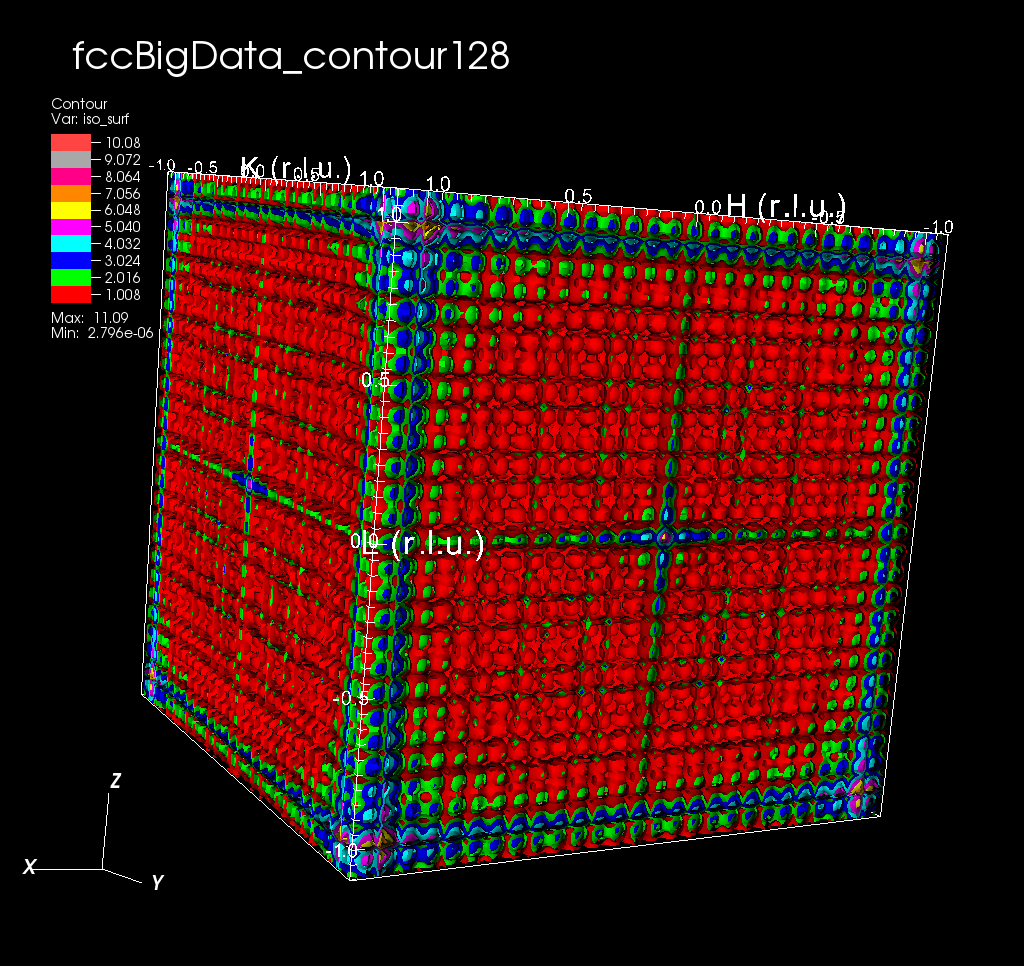
\includegraphics[width=1.\textwidth, ]{pics/fccBigData_contour128.png}
%                 \caption{synthetic scattering maps for $\gg 10^9$ atoms in 3D}
% %                 \caption{Interactive visualization of $|A(s)^{2}|$ in 3D with ParaView}
%             \end{figure}    
%             \end{column}
%         \end{columns}
% \end{frame}

%%%% 2ND VERSION %%%%

\begin{frame}
    \frametitle{GPU-accelerated analysis of large X-ray data}
    %\frametitle{Goals: Optimize analysis workflow for Big Data}
        \begin{enumerate}
                \item<1-> Direct calculation in \textcolor{red}{3D reciprocal space (hkl)}: \textbf{atomic positions} (${\bf r_{i}}$) $\&$ scattering factors ($f_{i}$):
                    \begin{itemize}
                        \hfsetfillcolor{blue!10}
                        \hfsetbordercolor{blue} 
                        \item \tikzmarkin<1>{fourier1}(0.2,-0.42)(0.2,0.6)$A({\bf s}) = \sum\limits_{j=0}^{N-1} f_{j}(s) e^{2i\pi {\bf S}\cdot {\bf r_{j}}}$\tikzmarkend{fourier1} \hspace*{5mm}\drWalley
                        \item computing any point in ($hkl$) from \textcolor{red}{any structural model!}
                    \end{itemize}
                \item<2-> In crystallography usually we have: 
                    \begin{itemize}
                        \item many atoms, e.g. \tikzmarkin<2>{atoms}(0.35,-0.2)(0.15,0.32)$N_{\rm atoms} ~ \mathcal{O}(\num{\geq1e8})$\tikzmarkend{atoms} \hspace*{5mm} \dAnnoey 
                        \item many reflections ($N_{\rm hkl}$) in $hkl$, 
                              e.g. $N_{\rm khl}~\mathcal{O}(128 \times 128 \times 128)$ 
                    \end{itemize}    
                \item<3-> It requires \textbf{massive parallelism} 
                % (ideally \num{>1e4} simultaneous identical calculations);
                    \begin{itemize}
                        \hfsetfillcolor{green!10}
                        \hfsetbordercolor{green}
                        \item \tikzmarkin<3>{flops}(0.2,-0.15)(-0.,0.3)$N_{\rm flop} \approx 10 \times N_{\rm atoms} \times N_{\rm hkl}: \mathcal{O}(\num{1e14})$\tikzmarkend{flops}~\textit{flop} \hspace*{5mm}\dNinja%floating point operations 
                        %\item $N_{\rm flop} >> N_{\rm memory ~ transfers}$;
                        \item \small modern GPU: $10^{13}$ Flop/s, CPU server: $10^{12}$ Flop/s \hspace*{5mm}\dWinkey
                        \item \small algorithm well suited for GPU computations, scalable across multiple GPUs $\rightarrow \mathcal{O}(minutes)$
                    \end{itemize}    
                \end{enumerate}
%            \hspace*{1.cm}
\end{frame}
%============================
% My Comments
% task: compute synthetic scattering maps 
% for 10^9 atoms in 3 dimensions
%============================

%--------------------------------------------------------------------
\section{Big Data Analytics at MPCDF}
% {%<--- Start local changes
% \setbeamertemplate{navigation symbols}{}
% \usebackgroundtemplate{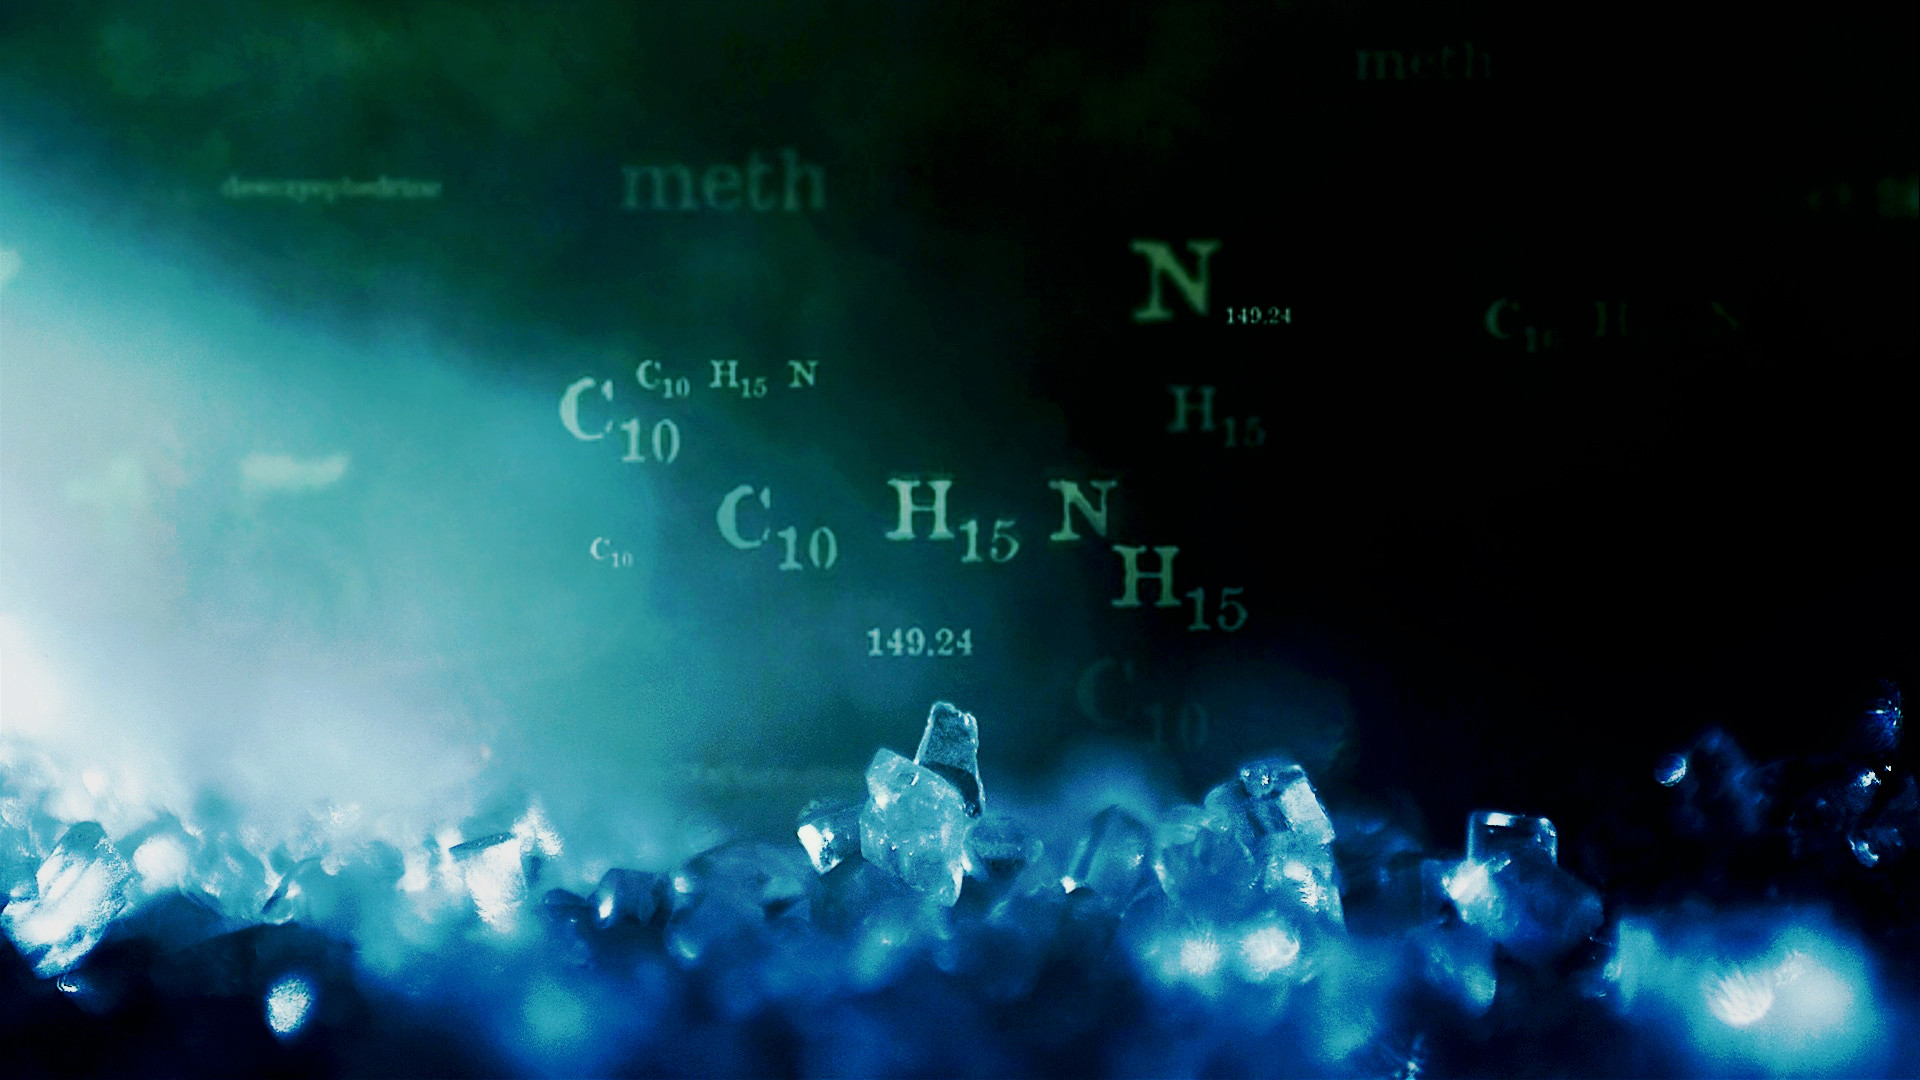
\includegraphics[width=\textwidth]{pics/meth}}
% \begin{frame}[plain]
% \end{frame}
% }%<---- Finish local changes
\begin{frame}[plain]
    \begin{tikzpicture}[remember picture,overlay]
        \node[at=(current page.center)] {
            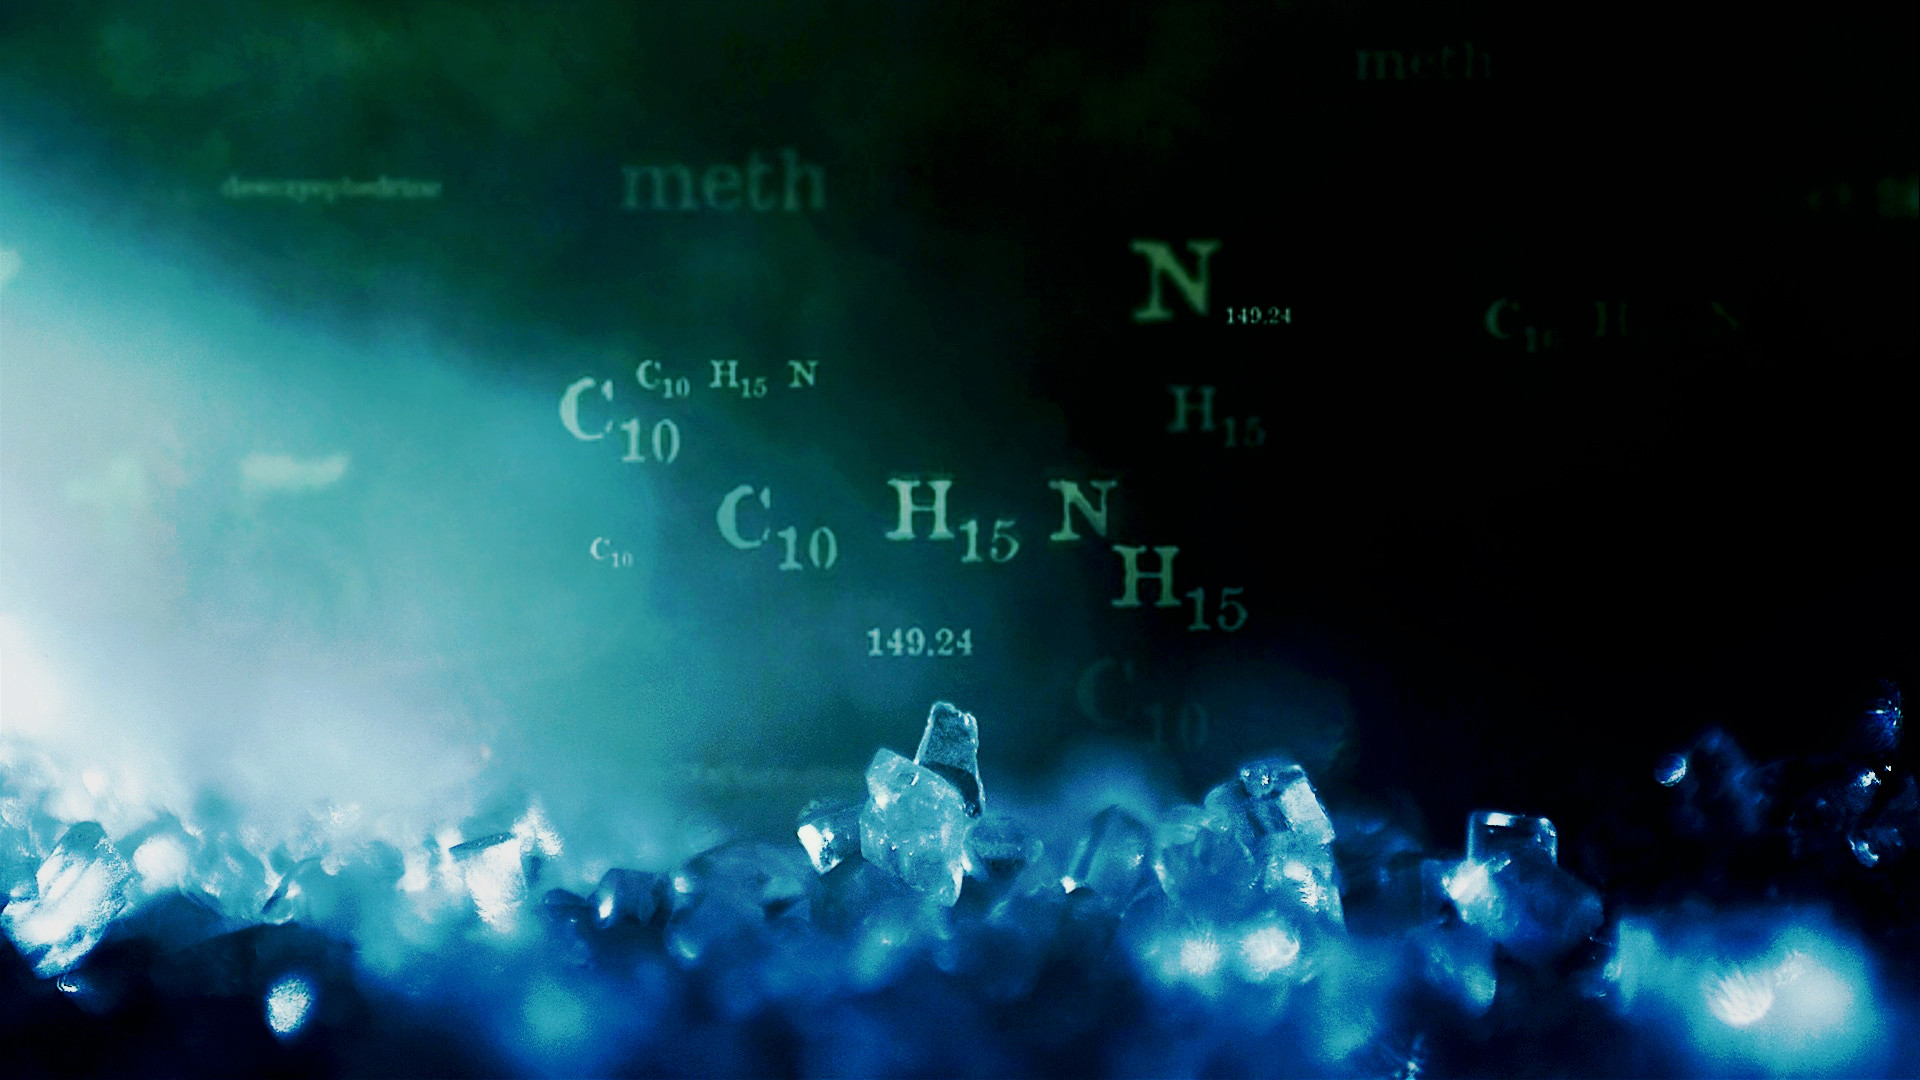
\includegraphics[width=\paperwidth, height=\paperheight]{pics/meth}
        };
    \end{tikzpicture}
    \Huge{\centerline{\textcolor{white}{Big Data Analytics at the MPCDF}}}

\end{frame}
%--------------------------------------------------------------------
\subsection{PyNX: A Python-based approach to GPU computing} 

%--------------------------------------------------------------------
\begin{frame}
\frametitle{PyNX: Tools for {\bf Nano-structures X-tallograhy}}
    \visible<1->{It is an open-source library created by \textit{Vincent Favre-Nicolin} at ESRF\footnotemark with the following main modules:
                \begin{enumerate}
                    \item \visible<2->{\tikzmarkin<2->{pynx.gpu}\texttt{pynx.gpu}\footnotemark: X-ray scattering computing using graphical processing units, allowing up to $4\times 10^{11}$ reflections/atoms/seconds (e.g., 2x nVidia GeForce GTX 980)\tikzmarkend{pynx.gpu};}
                    \item \visible<3->{\texttt{pynx.ptycho}: simulation and analysis of experiments using the ptychography technique;}
                    \item \visible<4->{\texttt{pynx.wavefront}: X-ray wavefront propagation in the near, far field, or continuous;}
                    \item \visible<5->{\texttt{pynx.cdi}: Coherent Diffraction Imaging reconstruction algorithms using GPU.}
                \end{enumerate} 
             \footnotetext[1]{European Synchrotron Radiation Facility; \url{favre@esrf.fr}}   
            \footnotetext[2]{{\bf New}: in PyNX 3.1.0, is called \texttt{pynx.scattering}}
            }
\end{frame}

%--------------------------------------------------------------------

\begin{frame}
\frametitle{PyNX: Hardware requirements}
PyNX aims to help computing scattering (X-ray or neutrons) maps for atomic structures, especially if they are \textit{distorted or disordered}.

% The library uses GPU computing (although parallel CPU computing is also available as a fall-back), with the following platforms:
% nVidia's CUDA toolkit and the pyCUDA library
% OpenCL language, along with pyOpenCL library.
% Using GPU computing, PyNX provides fast parallel computation of scattering from large assemblies of atoms (>> 108 atoms) and 1D, 2D or 3D coordinates (>>106 grid points)
% in reciprocal space. Typical computing speeds on GPUs more than 1011 reflections/atoms/s on nVidia cards, more than 2 orders of magnitude faster than on a CPU.

\begin{columns}
    \begin{column}{.8\textwidth}
        \begin{itemize}
            \item High-performance computing with GPUs
        %\begin{itemize}
        %    \item GPUs computing
                \begin{itemize}   
                    \item \textcolor{blue}{nVidia's CUDA toolkit}\footnotemark and the pyCUDA library
                    \item \textcolor{red}{OpenCL}\footnotemark language, along with pyOpenCL library     
                \end{itemize}  
        \end{itemize}
                \begin{block}{GPU-accelerated applications}
        \small \textcolor{blue}{PyNX provides fast parallel computation of \textit{scattering from large assemblies of atoms} ($\gg 10^{8}$ atoms) and \textbf{1D}, \textbf{2D} or \textbf{3D} coordinates ($\gg 10^{6}$ grid points) in \textit{reciprocal latticespace}.}
        \end{block}
        \vspace*{-0.31cm}
    \end{column}
    \begin{column}{.35\textwidth}
        \begin{figure}
            \begin{minipage}{0.65\textwidth}
                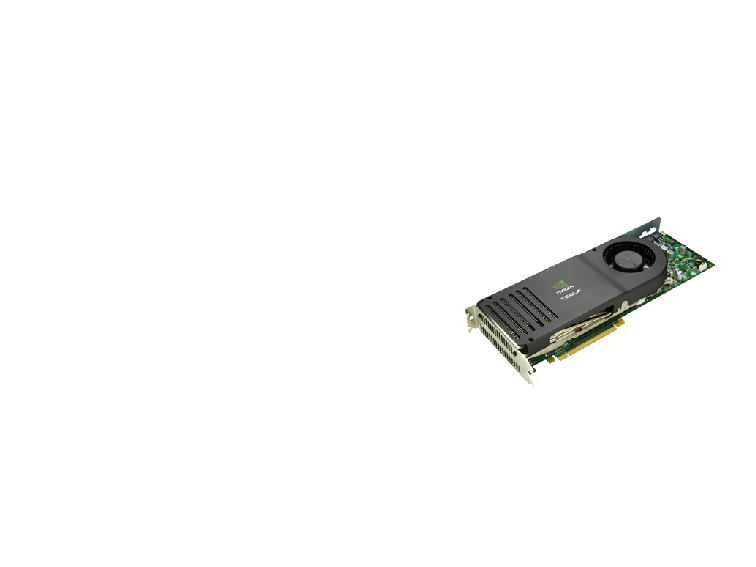
\includegraphics[width=\textwidth]
                {pics/tesla_card}
            \end{minipage}
        \end{figure}   
    \end{column}
    \hspace*{-1cm}
\end{columns}
\footnotetext[3]{\url{https://developer.nvidia.com/cuda-toolkit}}
\footnotetext[4]{\url{https://www.khronos.org/opencl/}}
\end{frame}

%--------------------------------------------------------------------

\begin{frame}[fragile]
\frametitle{PyNX: Software requirements}
PyNX supports Python version {\bf 2.7, 3.4} and above (\textcolor{green}{Anaconda distribution} is recommended).\\ 
\textcolor{blue}{Python interface} $\Rightarrow$ \textcolor{red}{No need to learn CUDA}

\begin{columns}
    \begin{column}{.7\textwidth}
              \hspace*{-1.5cm}
                \begin{block}{PyNX: Prerequisites}
        \small PyNX is available from:
\begin{itemize}
\item<1-> Mandatory: \texttt{numpy, matplotlib, pycuda};
\item<2-> Recommended\footnotemark: \texttt{pyfftw} for cpu calculations;
\item<3-> Optionally\footnotemark: \texttt{cctbx} library, for \textit{grazing incidence scattering} \\ 
\texttt{\$ conda install -c mx cctbx=20160309}
\end{itemize}
        \end{block}
        %\vspace*{-0.31cm}
    \end{column}
    \begin{column}{.3\textwidth}
            \begin{textblock}{5}(2.5,.88)
                \scriptsize\itshape{\textcolor{blue}{Python is the Common Language}}
            \end{textblock}
        %\begin{figure}
         %   \begin{minipage}{0.65\textwidth}
                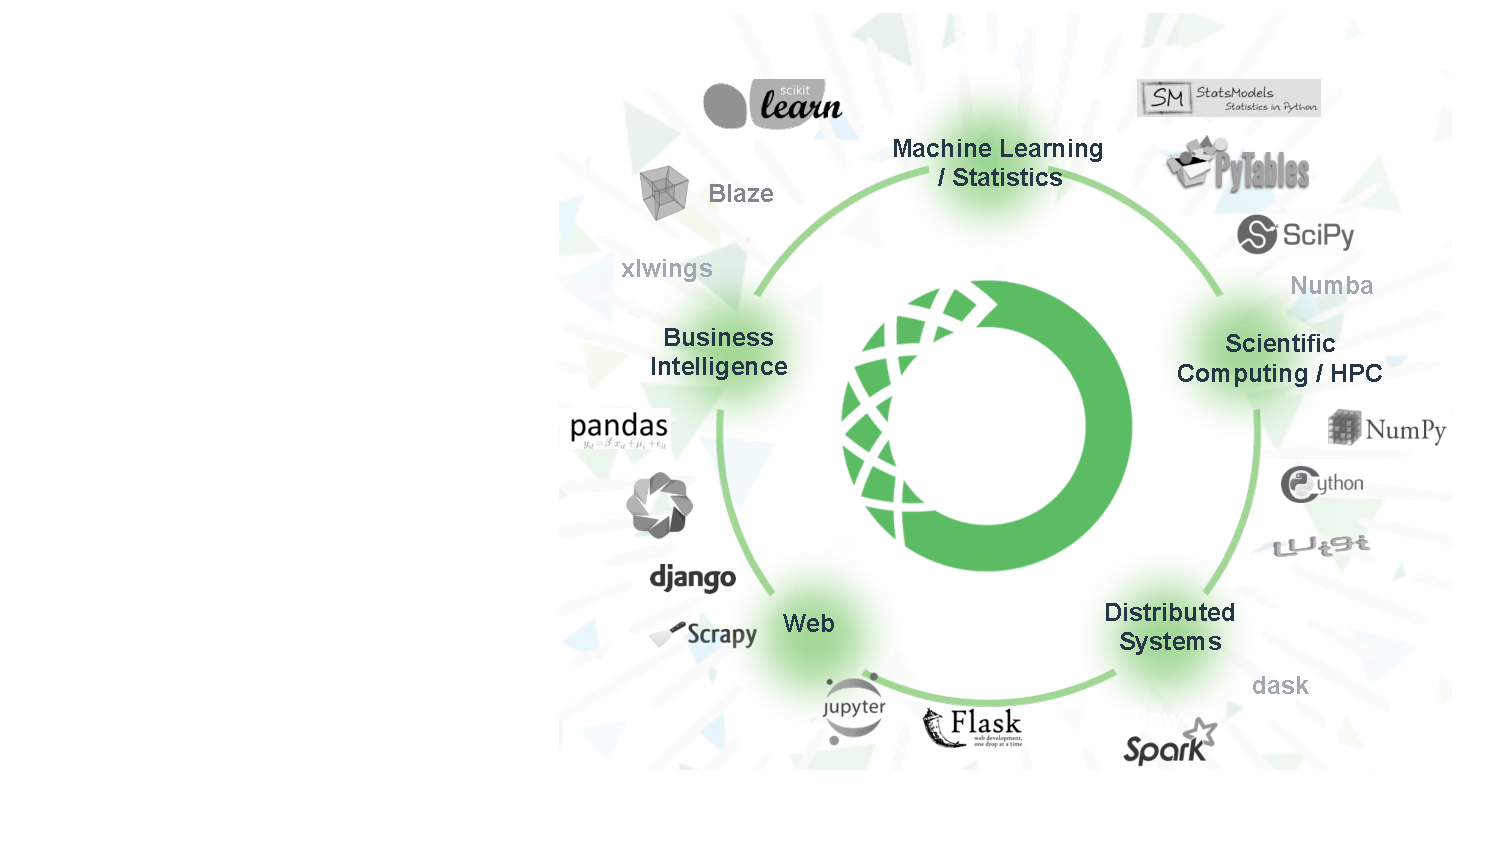
\includegraphics[width=1.3\textwidth]
                {pics/anaconda_distribution}
          %  \end{minipage}
        %\end{figure}   
    \end{column}
    \hspace*{.8cm}
\end{columns}
\footnotetext[6]{\url{https://pypi.python.org/pypi/pyFFTW}}
\footnotetext[7]{\url{http://cctbx.sourceforge.net/}}
\end{frame}

%--------------------------------------------------------------------
%--------------------------------------------------
\begin{frame}[fragile]
\frametitle{PyNX: Software requirements}
PyNX supports Python version {\bf 2.7, 3.4} and above (\textcolor{green}{Anaconda distribution} is recommended) .\\ 
\textcolor{blue}{Python interface} $\Rightarrow$ \textcolor{red}{No need to learn CUDA}

\begin{columns}
    \begin{column}{.7\textwidth}
%         \begin{itemize}
%             \item GPUs computing
%                 \begin{itemize}   
%                     \item \textcolor{blue}{nVidia's CUDA toolkit}\footnotemark and the pyCUDA library
%                     \item \textcolor{red}{OpenCL}\footnotemark language, along with pyOpenCL library     
%                 \end{itemize}  
%         \end{itemize}
              \hspace*{-1.cm}
                \begin{block}{Install PyNX}
        \small PyNX is available from:
\begin{itemize}
\item<1-> \url{http://ftp.esrf.fr/pub/scisoft/PyNX/}
\item<2-> \url{http://gitlab.esrf.fr/favre/PyNX} 
\item<3-> \texttt{PyPI}: \begin{verbatim}
$ pip install pynx
\end{verbatim}

\end{itemize}
        \end{block}
        \vspace*{-0.31cm}
    \end{column}
    \begin{column}{.3\textwidth}
        \begin{textblock}{5}(2.8,1.)
                \scriptsize\itshape{\textcolor{blue}{Python is also a great\\ glue language!}}
            \end{textblock}
        \begin{figure}
            \begin{minipage}{0.65\textwidth}
                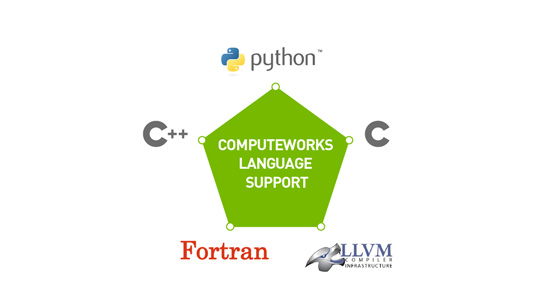
\includegraphics[width=2.4\textwidth]
                {pics/cuda-5}
            \end{minipage}
        \end{figure}   
    \end{column}
    \hspace*{1.cm}
\end{columns}
\end{frame}

% ========================
% My Comments: 
% High-level scripting languages are in many ways polar opposites to GPUs.
% GPUs are highly parallel, subject to hardware subtleties, and designed for
% maximum throughput, and they offer a tremendous advance in the performance
% achievable for a significant number of computational problems. On
% the other hand, scripting languages such as Python favor ease of use over
% computational speed and do not generally emphasize parallelism. PyCUDA
% is a package that attempts to join the two together
% ========================
\begin{frame}
\frametitle{Why do Scripting for GPUs?}
\hfsetfillcolor{green!10}
\hfsetbordercolor{green}
\begin{columns}
    \begin{column}{.65\textwidth}
        \begin{itemize}
            \item GPUs are everything that \textit{high-level scripting languages} \textbf{are not}.
                \begin{itemize}
                    \item Highly parallel
                    \item Very architecture-sensitive
                    \item Built for maximum FP/memory throughput \\$\rightarrow$ complement each other   
                \end{itemize}  
            % \item CPU: largely restricted to control tasks ($~1000/sec$)
            %     \begin{itemize}
            %         \item Scripting fast enough
            %     \end{itemize}
            % COMMENT: On the other hand, scripting languages favor ease of use over 
            % computational speed and do not generally emphasize parallelism
            % PyCUDA is a package that attempts to join the two togheter
            \item \small Scripting $+$ GPU : A good combination 
            \begin{center}$\Downarrow$\end{center}
            \item \tikzmarkin<1>{pycuda}Python + CUDA\footnotemark = \textbf{PyCUDA}\tikzmarkend{pycuda} 
            \item Python + OpenCL = \textbf{PyOpenCL} 
        \end{itemize}
    \end{column}
    \begin{column}{.45\textwidth}
        \begin{figure}
            \begin{minipage}{0.65\textwidth}
                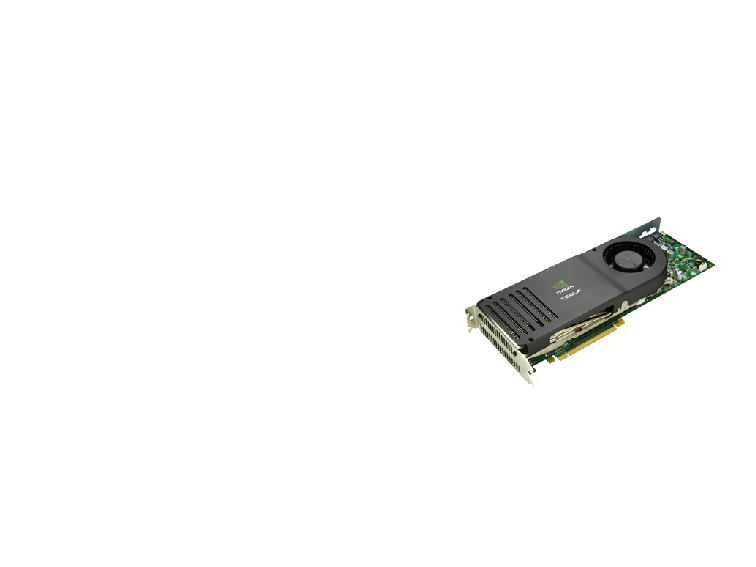
\includegraphics[width=\textwidth]{pics/tesla_card}
                \caption{courtesy by A. Kl\"{o}ckner, Nvidia GTC 2010}
            \end{minipage}
        \end{figure}   
    \end{column}
    \hspace*{-2cm}
\end{columns}
\footnotetext[8]{\scriptsize CUDA is a general purpose parallel computing architecture
that leverages the parallel compute engine\\ in NVIDIA graphics processing units (GPUs)}%to solve many complex computational problems in a fraction of the time required on a CPU.}
\end{frame}
% MY COMMENTS
% CUDA is a general purpose parallel computing architecture that leverages the parallel compute engine in NVIDIA graphics processing units (GPUs) to solve many complex computational problems in a fraction of the time required on a CPU. It includes the CUDA Instruction Set Architecture (ISA) and the parallel compute engine in the GPU. To program to the CUDATM architecture, developers can, today, use C, one of the most widely used high-level programming languages, which can then be run at great performance on a CUDATM enabled processor. Other languages will be supported in the future, including FORTRAN and C++.

% -------------------------------------------------------------------

\begin{frame}
\frametitle{But before PyCUDA: why Python at all?}
\begin{columns}
    \begin{column}{0.75\textwidth}
    \begin{itemize}
        \item general purpose \dCooley
        \item simple to learn and use \dSmiley % (interpreted)
        \item extensible and embeddable: Python C API
        \item science oriented too (NumPy, SciPy, mpi4py)
        \item great visualization tools (Bokeh, Matplotib) %\dCooley 
        \item very well documented 
    \end{itemize}
    \end{column}
    \begin{column}{.43\textwidth}
        \begin{figure}
            \begin{minipage}{1.\textwidth}
                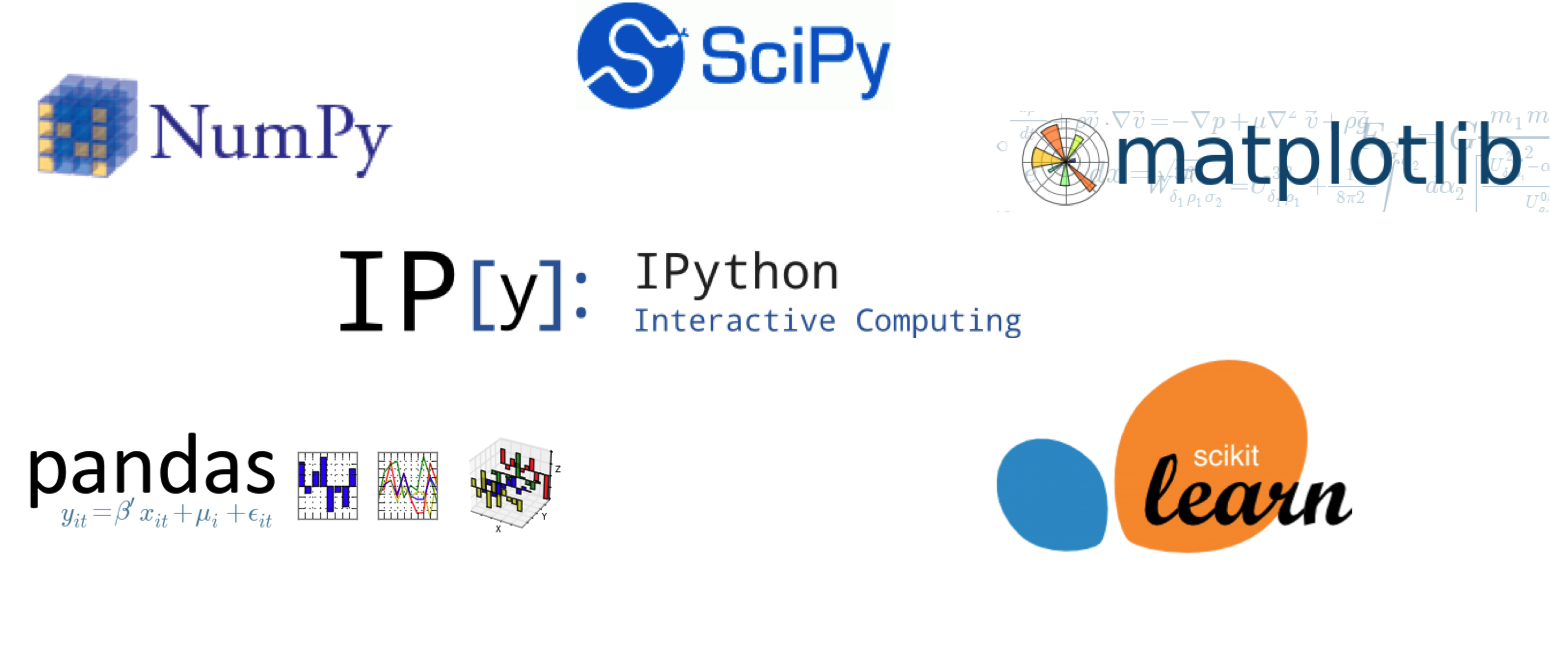
\includegraphics[width=1.\textwidth]{pics/logo-stack-python}
                %\caption{}
             \end{minipage}
        \end{figure}
    \end{column}
    \hspace*{1.2cm}
\end{columns} 
    \vfill
    \vspace*{-0.1cm}
    \begin{block}{NumPy: package for large, N-dimensional array object \dCooley}
    \begin{itemize}
        \item \small \texttt{Vectors, Matrices, ...} array computing is fast
        \item \small \texttt{A+B, sin(A), dot(A,B)}
        \item \small \texttt{la.solve(A,b), la.eig(A)}
        \item \small \texttt{cube[;, ;, n-k:n+k], cube+5}
        \item \small \texttt{FFT's}, tools for integrating \texttt{C/C++} and \texttt{Fortran} code
    \end{itemize}   
\end{block}
%==================
% My comments
% NumPy is the fundamental package for scientific computing with Python. It contains among other things:

%     a powerful N-dimensional array object
%     sophisticated (broadcasting) functions
%     tools for integrating C/C++ and Fortran code
%     useful linear algebra, Fourier transform, and random number capabilities

% Besides its obvious scientific uses, NumPy can also be used as an efficient multi-dimensional container of generic data. Arbitrary data-types can be defined. This allows NumPy to seamlessly and speedily integrate with a wide variety of databases.
\end{frame}


%--------------------------------------------------------------------

\begin{frame}
\frametitle{Scripting: Python\footnote{Slide courtesy by A. Kl\"{o}ckner, Nvidia GTC 2010}}
One example of a scripting language: Python

\begin{columns}
    \begin{column}{.5\textwidth}
        \begin{itemize}
            \item Mature
            \item Large and active community
            \item Emphasizes readability
            \item Written in widely-portable C 
            \item A 'multi-paradigm' language
            \item Rich ecosystem of sci-comp related software
        \end{itemize}
    \end{column}
    \begin{column}{.5\textwidth}
        \begin{figure}
            \begin{minipage}{0.65\textwidth}
                
\includegraphics[width=0.85\textwidth]{pics/python_logo}
                %\caption{courtesy by A. Kl\"{o}ckner, Nvidia GTC 2010}
            \end{minipage}
        \end{figure}   
    \end{column}
    \hspace*{-2cm}
\end{columns}
\end{frame}

%====================================================================
% The PyCUDA philosophy
%{\bf PyCUDA} gives you easy, Pythonic \underline{complete} access to Nvidia's CUDA parallel computation API. \\ Some PyCUDA \textbf{features}:

\begin{frame}
\frametitle{PyCUDA Philosophy: maps all CUDA into Python}
    \visible<1->{{\bf PyCUDA} lets you completely access to Nvidia's CUDA parallel computation API from Python.}
    \visible<2->{\textbf{Key Features}:}
    \visible<2->{
        \begin{columns}
            \begin{column}{.7\textwidth}
                \begin{itemize}
                    \item \visible<3->{{\bf Robustness}: automatic management of object lifetimes and  error checking} %{Automatically manage resources}
                    \item \visible<4->{{\bf Completeness}: automatic error checking}
                          %Check for and report errors automatically}
                    \item \visible<5->{{\bf Convenience}: provide abstractions (comes with ready-made on-GPU linear algebra, reduction, scan. Add-on packages for FFT and LAPACK available.)} % high-level of abstractions: GPUArray for example
                    \item \visible<6->{Integrate tightly with \texttt{\bf NumPy}}
                    \item \visible<7->{{\bf Speed}: PyCUDA’s base layer is written in \texttt{C++} (near-zero wrapping overhead)}
                    \item \visible<8->{Complete, helpful \href{https://documen.tician.de/pycuda/}{\underline{documentation}}} 
%           \href[\underline{documentation}]{https://documen.tician.de/pycuda/} and \href[Wiki]{https://wiki.tiker.net/PyCuda}}
                \end{itemize} 
            \end{column}
            \visible<2->{\begin{column}{.3\textwidth}
                \begin{figure}
                    \begin{minipage}{0.65\textwidth}
                        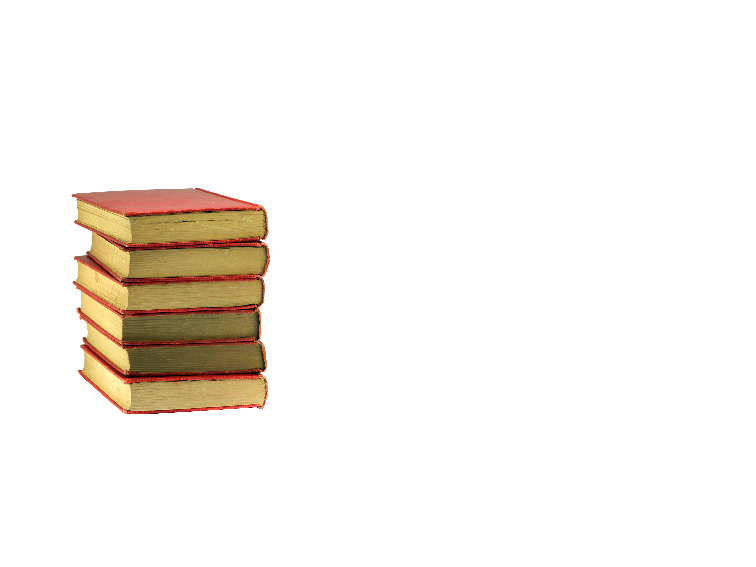
\includegraphics[width=1.2\textwidth]{pics/pycuda_philosophy}
                        %\caption{}
                    \end{minipage}
                \end{figure}
            \end{column}
            }
        \end{columns}
        }
\end{frame}

% ===============
% My comments 
% ===============
% Enables run-time code generation (RTCG) for flexible, fast, automatically tuned codes.
% Added robustness: automatic management of object lifetimes, automatic error checking
% Added convenience: comes with ready-made on-GPU linear algebra, reduction, scan. Add-on packages for FFT and LAPACK available.
% Fast. Near-zero wrapping overhead.
%  Complete, helpful documentation.
% 0. Maps all of CUDA into Python.
% 1. PyCUDA is a Python scripting language wrapper around the CUDA C extension to the C programming language. PyOpenCL is the analogous wrapper around OpenCL for Python.        
% 2. Completeness. PyCUDA puts the full power of CUDA’s driver API at your disposal, if you wish.        
% 3. Object cleanup tied to lifetime of objects. This idiom, often called RAII in C++, makes it much easier to write correct, leak- and crash-free code. 
% PyCUDA knows about dependencies, too, so (for example) it won’t detach from a context before all memory allocated in it is also freed.
% Automatic Error Checking. All CUDA errors are automatically translated into Python exceptions.
% (e.g., \texttt{pycuda.compiler.SourceModule} and \texttt{pycuda.gpuarray.GPUArray}) % Convenience. Abstractions like pycuda.compiler.SourceModule and pycuda.gpuarray.GPUArray make CUDA programming even more convenient than with Nvidia’s C-based runtime.
% Speed. PyCUDA’s base layer is written in C++, so all the niceties above are virtually free.
% Helpful Documentation.

% %--------------------------------------------------------------------

% \begin{frame}
% \frametitle{Scripting: Interpreted, not Compiled}
% Program creation workflow:
% \begin{figure}
%     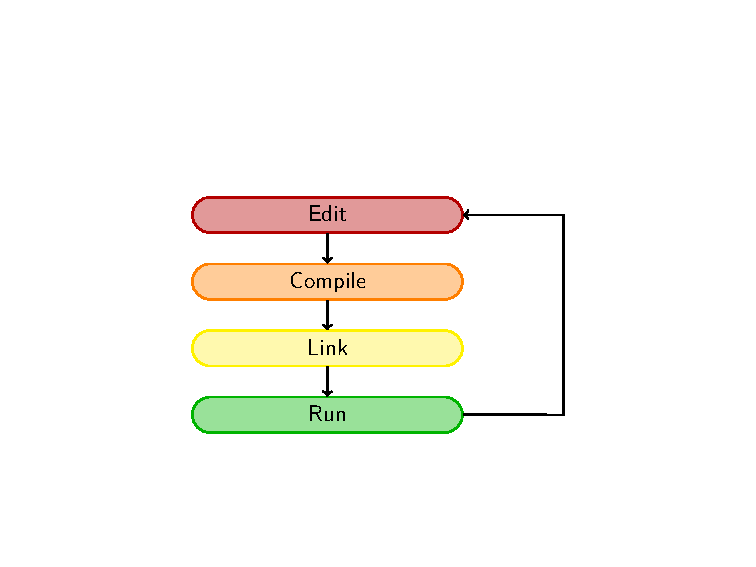
\includegraphics[width=0.65\textwidth]{pics/workflow}
%         \caption{courtesy by A. Kl\"{o}ckner, Nvidia GTC 2010}
% \end{figure}
% \end{frame}

% %--------------------------------------------------------------------

% \begin{frame}
% \frametitle{Scripting: Interpreted, not Compiled}
% Program creation workflow:
% \begin{figure}
%     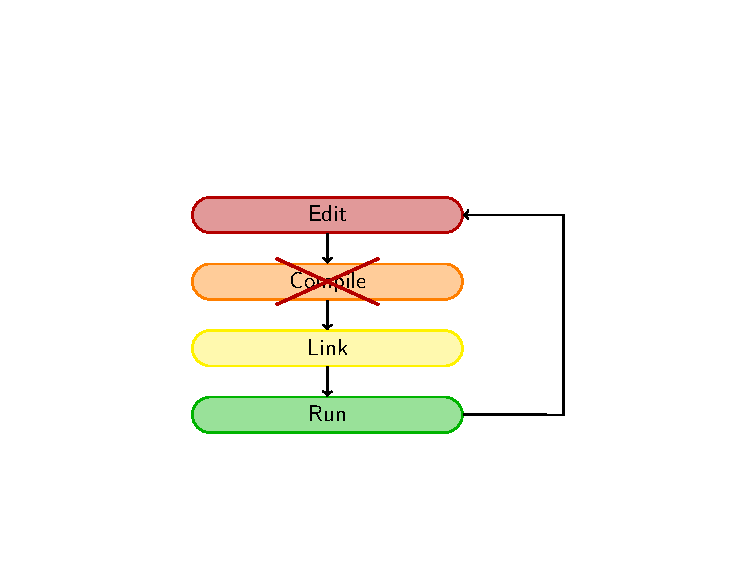
\includegraphics[width=0.65\textwidth]{pics/workflow1}
%         \caption{courtesy by A. Kl\"{o}ckner, Nvidia GTC 2010}
% \end{figure}
% \end{frame}

% %--------------------------------------------------------------------
% \begin{frame}
% \frametitle{Scripting: Interpreted, not Compiled}
% Program creation workflow:
% \begin{figure}
%     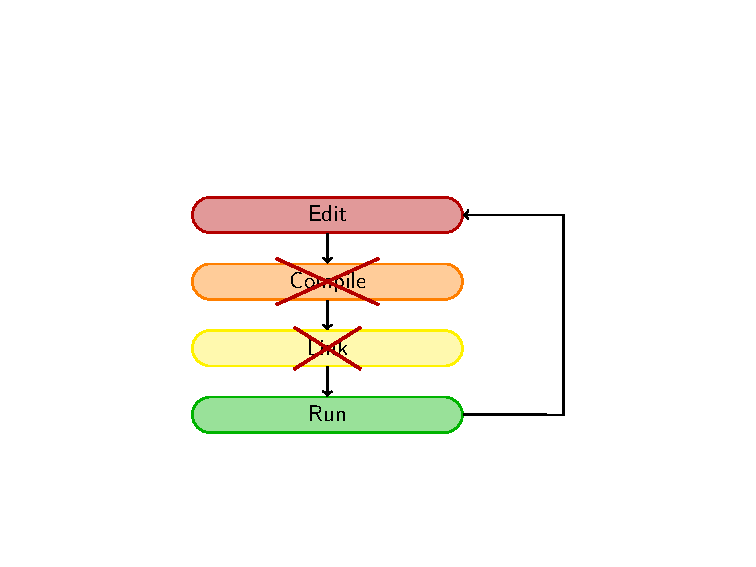
\includegraphics[width=0.65\textwidth]{pics/workflow2}
%         \caption{courtesy by A. Kl\"{o}ckner, Nvidia GTC 2010}
% \end{figure}
% \end{frame}

%--------------------------------------------------------------------

\begin{frame}
%\hfsetfillcolor{blue!10}
%\hfsetbordercolor{blue}
%(0.2,-0.5)(-0,0.7)
    \frametitle{Whetting your appetite: \texttt{SourceModule}}
        \begin{columns}
            \begin{column}{\textwidth}
                \ttfamily\footnotesize
                {\bf import} \textcolor{red}{pycuda}.driver as \textcolor{red}{cuda}\\
                {\bf import} \textcolor{red}{pycuda}.autoinit\\
                {\bf import} \textcolor{red}{numpy} as \textcolor{red}{np}
                
                a = \textcolor{red}{np}.random.randn(4,4).astype(\textcolor{red}{np}.float32)\\
                a\_gpu = \textcolor{red}{cuda}.mem\_alloc(a.nbytes) \\
                \# \textit{host-to-device}\\
                \textcolor{red}{cuda}.memcpy\_htod(a\_gpu, a) \\
                \vspace{2mm}
                mod = \textcolor{red}{cuda}.SourceModule("""\\
                    \tikzmarkin<1>{a}\textcolor{blue}{\_\_global\_\_ void multiply\_by\_two(float *a)\\
                    \texttt{\{}\\
                    int idx = threadIdx.x + threadIdx.y*4;\\
                    a[idx] *= 2;\\
                    \texttt{\}}}
                    \hfill \textsc{Compute Kernel}\tikzmarkend{a} \\
                    """)\\
                    \vspace{2mm}
                    func = mod.get\_function("\textcolor{blue}{multiply\_by\_two}")\\
                    func(a\_gpu, bloc=(4,4,1))
            \end{column}
%             \begin{column}{0.35\textwidth}
%                 \footnotesize
%                 {\bf import} \textcolor{red}{numpy} as \textcolor{red}{np}\\
%                 {\bf import} \textcolor{red}{pycuda}.autoinit\\
%                 {\bf import} \textcolor{red}{pycuda}.gpuarray as gpuarray\\
                
%             \end{column}
        \end{columns}
\end{frame}
%------------------------------------------------

\begin{frame}
    \frametitle{Whetting your appetite: \texttt{GPUArrays}}
        \ttfamily\footnotesize
        {\bf import} \textcolor{red}{numpy} as \textcolor{red}{np}\\
        {\bf import} \textcolor{red}{pycuda}.autoinit\\
        {\bf import} \textcolor{red}{pycuda}.gpuarray as gpuarray \\
        \vspace{.5mm}
     
        a\_gpu = gpuarray.to\_gpu(\textcolor{red}{np}.random.randn(4,4).astype(np.float32))\\
        a\_doubled = (2*a\_gpu).get() \\ 
        {\bf print} a\_doubled\\
        {\bf print} a\_gpu   
%        \begin{textblock}{2}(2,1)
%         \textblocklabel{block two}
% Here is another, slightly narrower, block, at position (2,1) on the page.
% \end{textblock}
\begin{block}{\texttt{GPUArrays}: computational linear algebra}
\begin{itemize}
\sffamily
\item \small element-wise algebraic operations (\texttt{+, -, *, /, sin, cos, exp})
% \item \small 
\item tight integration with \texttt{numpy}
\begin{itemize}
\item \small \texttt{gpuarray.to\_gpu(numpy\_array)}
\item \small \texttt{numpy\_array = gpuarray.get()}
\end{itemize}
\item \small mixed data types (\texttt{int32 + float32 = float64})
\end{itemize}
 

\end{block}
\end{frame}

%--------------------------------------------------------------------
\begin{frame}
\frametitle{PyCUDA Workflow: "Edit-Run-Repeat"}
A two-fold aim: 
\begin{enumerate}
    \item usage of \textit{existing} \texttt{CUDA C}
    \item \textit{on top} of the first layer, PyCUDA $\Rightarrow$ \textit{abstractions}
\end{enumerate}
\begin{figure}
    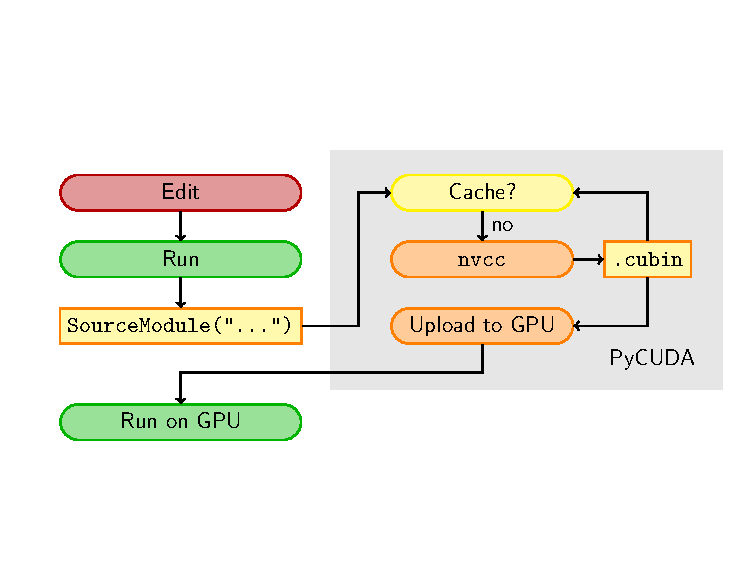
\includegraphics[width=0.95\textwidth]{pics/pycuda_workflow}
        \caption{A. Kl\"{o}ckner et al. 2013, \url{https://arxiv.org/abs/1304.5553}}
\end{figure}
\end{frame}

%--------------------------------------------------------------------

\subsection{PyCUDA}
\begin{frame}
\frametitle{PyCUDA: Vital Information}
\begin{columns}
    \begin{column}{.65\textwidth}
        \begin{itemize}
            \item Availability: \href{https://pypi.python.org/pypi/pycuda}{Freely down-loadable from this location}
                \begin{itemize}
                    \item Open source
                    \item MIT Licensed  
                \end{itemize}  
            \item requires {\bf NumPy}, Python 2.4+ (Win/OS X/Linux)
            \item Support via mailing list
            \item For further information see:
                \begin{itemize}
                    \item \href{https://mathema.tician.de/software/pycuda/}{Main PyCUDA page}
                   \item \href{https://wiki.tiker.net/PyCuda}{PyCUDA Wiki}
                   \item \href{https://wiki.tiker.net/PyCuda/FrequentlyAskedQuestions}{PyCUDA FAQ}
                \end{itemize}
        \end{itemize}        
    \end{column}
    \begin{column}{.45\textwidth}
        \begin{figure}
            \begin{minipage}{0.65\textwidth}
                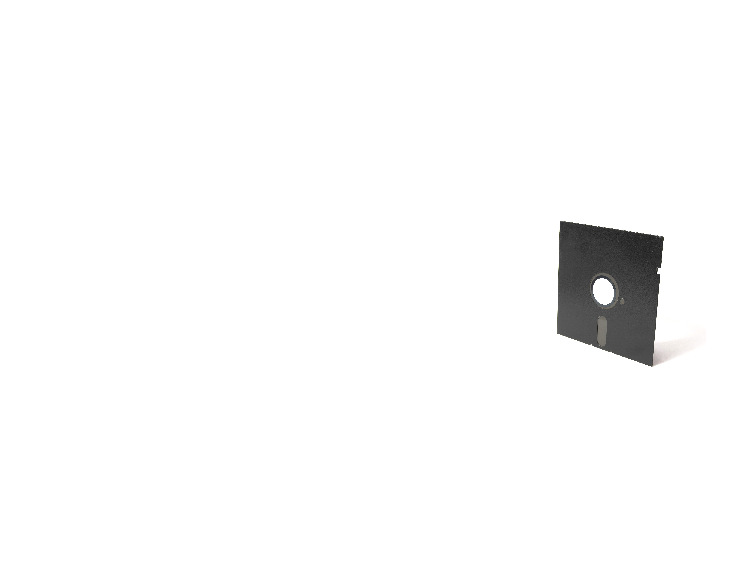
\includegraphics[width=1.1\textwidth]{pics/pycuda_vital}
                \caption{courtesy by A. Kl\"{o}ckner, Nvidia GTC 2010}
            \end{minipage}
        \end{figure}   
    \end{column}
    \hspace*{-2cm}
\end{columns}
\end{frame}

%------------------------------------------------



%---------------------------------------------------
\begin{frame}[fragile]
\frametitle{PyNX \textbf{kernel}: \texttt{\_\_global\_\_ void CUDA\_fhkl()}}
\lstset{language=C++, basicstyle=\ttfamily\scriptsize,commentstyle=\itshape\color{colComments}}
\begin{lstlisting}
const unsigned long ix=threadIdx.x+blockDim.x*blockIdx.x; // Thread idx
const float h=twopi*vh[ix];
const float k=twopi*vk[ix];
const float l=twopi*vl[ix];
float fr=0,fi=0;
__shared__ float x[BLOCKSIZE]; // Shared memory between BLOCKSIZE %d  
__shared__ float y[BLOCKSIZE]; // parallel threads
__shared__ float z[BLOCKSIZE];
long at=0;
for (;at<=(natoms-BLOCKSIZE);at+=BLOCKSIZE) { 
  __syncthreads();
  x[threadIdx.x]=vx[at+threadIdx.x]; // "Coalesced" transfer 
  y[threadIdx.x]=vy[at+threadIdx.x]; // to shared memory
  z[threadIdx.x]=vz[at+threadIdx.x];
  __syncthreads();
  for(unsigned int i=0;i<BLOCKSIZE;i++) {// Each thread computes
     float s,c;                              // a single reflection
     __sincosf(h*x[i] + k*y[i] + l*z[i] , &s,&c);  
     fr +=c; // fast, intrensic trigonometric function
     fi +=s;
  }__syncthreads();} 	
\end{lstlisting}
\end{frame}

%-------------------------------------------------

%---------------------------------------------------
\begin{frame}[fragile]
\frametitle{PyNX \textbf{kernel}: \texttt{\_\_global\_\_ void CUDA\_fhkl()}}
\lstset{language=C++, basicstyle=\ttfamily\scriptsize,commentstyle=\itshape\color{colComments}}
\begin{lstlisting}
__syncthreads()
;}

/* Take care of remaining atoms */
if(threadIdx.x<(natoms-at)) {
    x[threadIdx.x]=vx[at+threadIdx.x]; 
    y[threadIdx.x]=vy[at+threadIdx.x];
    z[threadIdx.x]=vz[at+threadIdx.x];
}
__syncthreads();
for(long i=0;i<(natoms-at);i++) {
    float s,c;
    __sincosf(h*x[i] + k*y[i] + l*z[i] , &s,&c);
    fr +=c;
    fi +=s;
}
fhkl_real[ix]+=fr;
fhkl_imag[ix]+=fi;
}
\end{lstlisting}
\end{frame}

%-----------------------------------------------
\begin{frame}[fragile]
\frametitle{PyNX \textbf{Python interface}: loading the data}
%A Python chunk code: 1) loading the data
\begin{lstlisting}
import numpy as np
import time 

@timeit
def do_work(*args, **kwargs):     
  def read_pos(file_name):
      """Loads an APT.pos file 
         Columns: x, y, z, Da
      """
      print("reading in the data")
      f = open(file_name, mode='rb') # Load orthonormal coord.
      dt_type = np.dtype({'names':['x', 'y', 'z', 'Da'],
                          'formats':['>f4', '>f4', '>f4', '>f4']})
      pos = np.fromfile(f, dt_type, -1)
      f.close()
      print("the data contain: {0:.5e} atoms".format(pos.size))
      return pos
\end{lstlisting}
\end{frame}

%-------------------------------------------------

\begin{frame}[containsverbatim]
\frametitle{PyNX Python interface: parsing the data}
%A Python chunk code: 2) parsing the data % \py{crystal.py}
    \begin{lstlisting}[firstnumber=16]
    if args[1] is not None:
        fname = args[1]

    df = readpos(fname)	
    xEl = df['x'] # slicing columns by labels
    yEl = df['y']
    zEl = df['z']
    lattice_parameter = 0.4045
    xEl /= lattice_parameter  # Convert to fractional coordinates
    yEl /= lattice_parameter 
    zEl /= lattice_parameter 
    N = 128
    h = np.linspace(-1.1, 1.1, num=N, endpoint=True) # HKL as 3D
    k = np.linspace(-1.1, 1.1, num=N, endpoint=True)[:, np.newaxis]
    l = np.linspace(-1.1, 1.1, num=N, endpoint=True)[:, np.newaxis, np.newaxis]
     \end{lstlisting}
\end{frame}

%-------------------------------------------------

\begin{frame}[fragile]
\frametitle{PyNX Python interface: The Fourier Transform}
% A Python chunk code: The Fourier transform
\begin{lstlisting}[firstnumber=31]
    from pynx import gpu  # main module for scattering computation
    gpu_name = args[0]  # identify GPU, e.g. GeForce GTX980  
    
    if args[0] is not None:
        fhkl, dt = gpu.Fhkl_thread(h, k, l, xEl, yEl, zEl,   gpu_name=args[0],verbose=True,language="CUDA",cl_platform="nvidia")
        print("The FT computed in dt = {0:7.5f}:".format(dt))
        print("{0:d} fourier number points".format(fhkl.size))
        
    return fhkl # a numpy complex64 array  
\end{lstlisting}
\begin{block}{\texttt{gpu.Fhkl\_thread}}
\begin{itemize}
\item \small computes \tikzmarkin<1>{fourier}(0.25,-0.2)(-0.1,0.35)$F(hkl) = \sum_{i}\exp[2j\pi(x_{i}\times h + y_{i} \times k + z_{i} \times l)]\tikzmarkend{fourier}$;
\item \small distributes the scattering maps on \textbf{several GPU}.
%\item \small creates a data volume (\texttt{h.size $\times$ k.size $\times$ l.size}): a numpy complex64 array
\end{itemize}
\end{block}
\end{frame}

%-------------------------------------------------

\begin{frame}
\frametitle{PyNX: Performance }
    \begin{columns}
        \begin{column}{0.5\textwidth}
            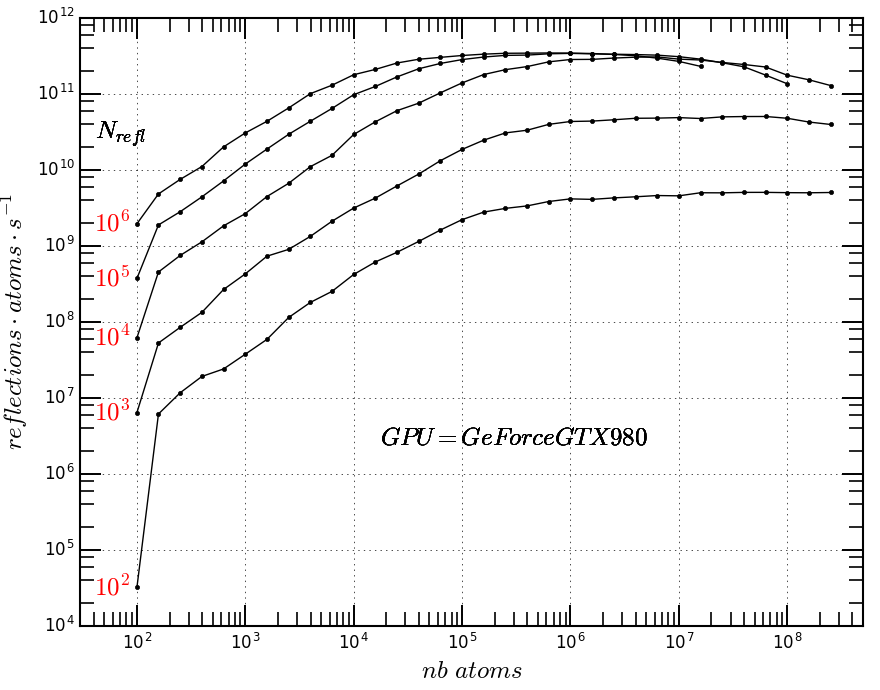
\includegraphics[width=1.2\textwidth]{pics/GPU-GeForce_GTX_980-speed.png}
        \end{column}
        \hspace*{5mm}
        \begin{column}{0.5\textwidth}
            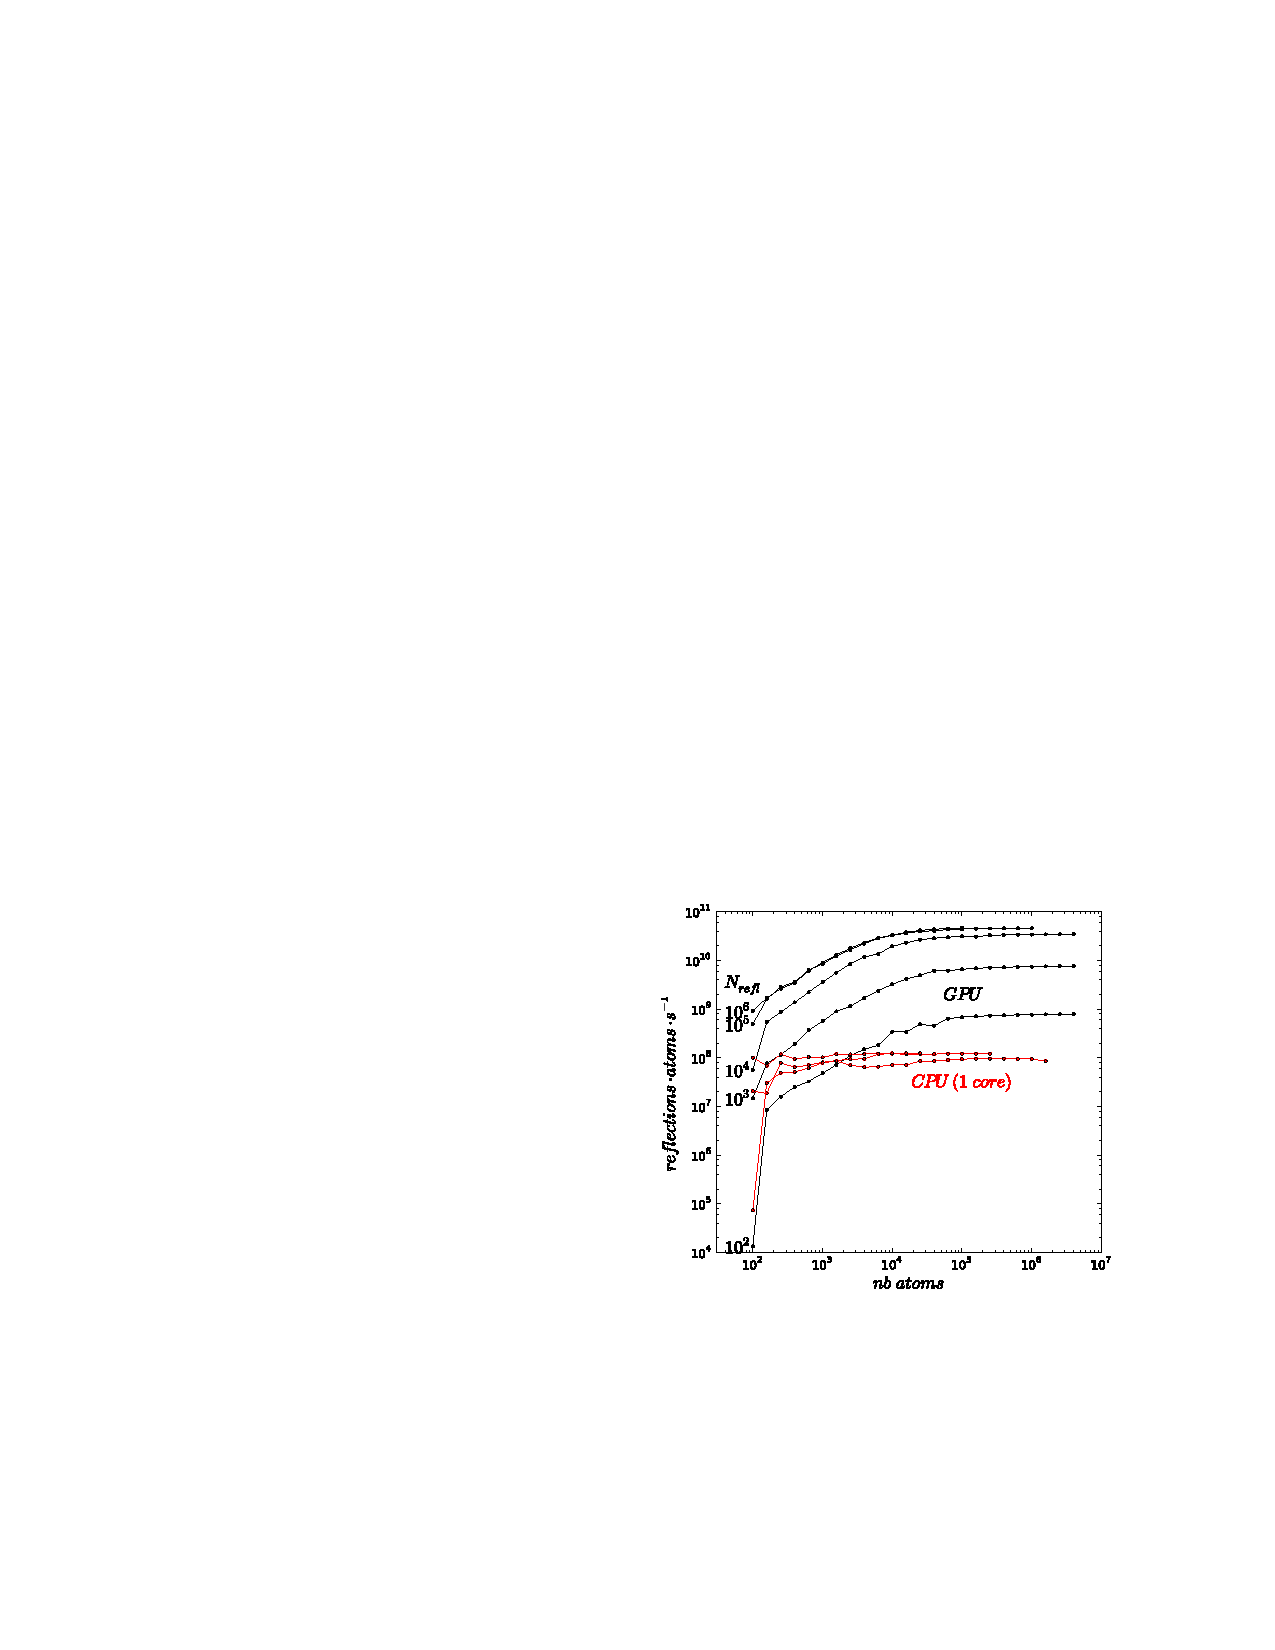
\includegraphics[width=1.08\textwidth]{pics/favre_pynx-test.pdf}
        \end{column}
    \end{columns}
    \begin{textblock}{5}(2.5,1.5)
       \scriptsize\itshape{cf. Favre-Nicolin et al.,\\ J. Appl. Cryst. 44 (2011) 635}
    \end{textblock}
    \begin{block}{assesment of \textbf{GPU-accelerated python} software package PyNX}
        \begin{itemize}
            \item \small Effective (singe precision) throughput per GPU: \\ 
             up to \textbf{$3.5\times 10^{11}$ reflections $\cdot$ atoms $\cdot$ s$^{-1}$}  
            %\item \small What is the peak performance???
        \end{itemize}
    \end{block}
\end{frame}

%-------------------------------------------------

\begin{frame}
\frametitle{PyNX: benchmarks at the MPCDF}
\begin{columns}
\column{0.5\textwidth}
\begin{minipage}[c][0.4\textheight][c]{\linewidth}
  \centering
  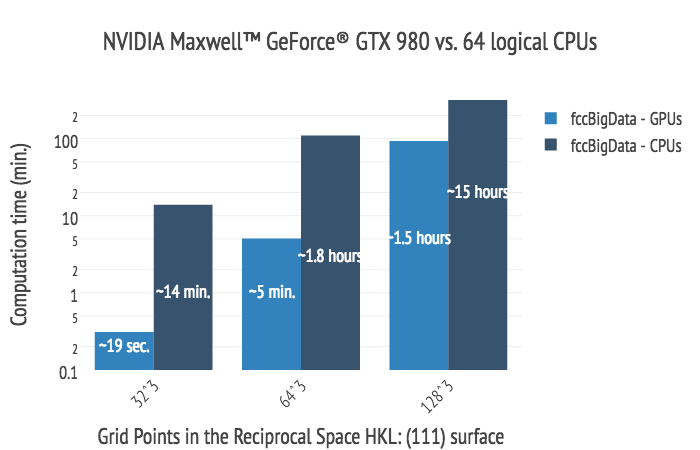
\includegraphics[width=0.8\linewidth]{pics/PyNX_runtest_DRACOgpu.png}
\end{minipage}
\begin{minipage}[c][0.4\textheight][c]{\linewidth}
  \centering
  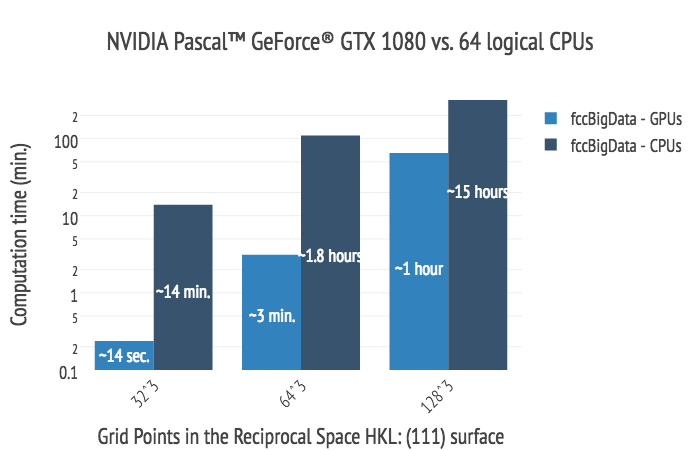
\includegraphics[width=0.8\linewidth]{pics/PascalGPUvsCPU.png}

\end{minipage}
\column{0.5\textwidth}
\begin{minipage}[c][0.4\textheight][c]{\linewidth}
  \textbf{PyNX computing time at the MPCDF for $10^{8}$ atoms}
  \begin{enumerate}
  \item 2 $\times$ nVidia GTX 980   
  \item 2 $\times$ nVidia GTX 1080
  \item interactive plots with Plotly 
  \end{enumerate}
\end{minipage}
\begin{minipage}[c][0.4\textheight][c]{\linewidth}
  \centering
  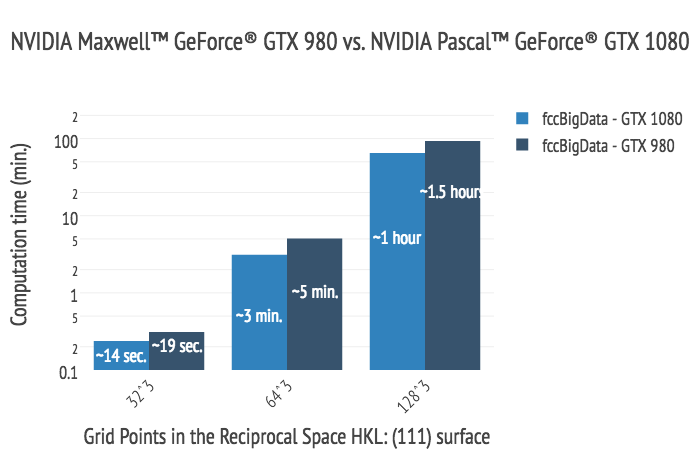
\includegraphics[width=0.8\linewidth]{pics/PyNX_runtest_PascalvsMaxwell_gpu.png}
\end{minipage}
\end{columns}
\end{frame}

\begin{frame}
\frametitle{Deploying Data Science Projects - Clusters}
%\frametitle{Here comes the Data Science - and it's all right}

\begin{columns}
    \hfsetfillcolor{lightgray}
    \hfsetbordercolor{gray!10} 

    \begin{column}{0.65\textwidth}
        \ttfamily\scriptsize
            % \begin{textblock}{5}(2.5,.8)
            % \textcolor{blue}{The SLURM workload manager}
            % \end{textblock}
            \tikzmarkin<1>{s}(1.2,-0.33)(-0.1,0.4)\#$!$/bin/bash -l\\
            \#SBATCH -J pynx\_run \\
            \# Queue:\\
            \#SBATCH --partition=gpu\\
            \# Node feature:\\
            \#SBATCH --constraint=\textcolor{yellow}{"gpu"}\\
            
            \# N. of nodes and MPI tasks per node:\\
            \#SBATCH --nodes=\textcolor{purple}{1}\\
            \#SBATCH --ntasks-per-node=\textcolor{purple}{32}\\
            \# wall clock limit:\\
            \#SBATCH --\textcolor{red}{time}=\textcolor{purple}{02:00:00} \\

            %\# Run the program:\\
            echo "starting the job ..."\\
            python crystAl.py -g="GeForce GTX 980"\tikzmarkend{s}\\
            echo "...done"
        \begin{block}{SLURM worload manager: basic usage}
        \begin{itemize}
            \item \small \texttt{qsub}: submit your job;
            \item \small \texttt{qstat}: query queue/job status;
            \item \small \texttt{qdel}: delete your job 
        \end{itemize}
        \end{block}
    \end{column}

    \begin{column}{0.45\textwidth}
        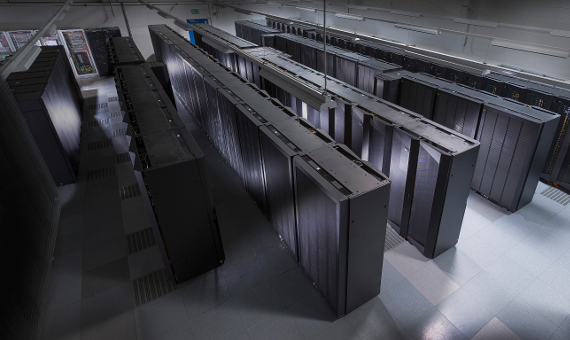
\includegraphics[width=1.1\textwidth]{pics/Hydra570.png}
        \begin{textblock}{5}(2.25,.5)
            \footnotesize\scshape{\textcolor{red}{Supercomputing Drives\\ Science through Simulations}}
        \end{textblock}
        \begin{textblock}{5}(2.5,2.2)
            \scriptsize\itshape{\textcolor{blue}{The MPG SuperComputer \textit{Hydra}\\ at the MPCDF}}
        \end{textblock}
    \end{column}

\end{columns}
\end{frame}
%--------------------------------------------------------------------
\section{Visualization of Crystal Nano-Structure}
% \begin{textblock}{5}(1.5, .4)
%     \footnotesize\itshape{The simple graph has brought more information\\ to the data analyst's mind than any other device.}\\
%                           - John Tukey in \textbf{The Future of Data Analysis}
% \end{textblock}
%--------------------------------------------------------------------

\subsection{Python Plotting for Exploratory Data Analysis}%{Data Visualization: Image Processing in Python}
\begin{frame}
\frametitle{Image Processing in Python: Toolbox for SciPy}
    %\hfsetfillcolor{lightgray}
    %\hfsetbordercolor{gray!2}
    %\tikzmarkin<1>{im}(2.2,-0.33)(-0.1,0.4)
    %\tikzmarkend{im}
        % \begin{block}
        % \begin{itemize}
        % \item Marching cubes is an algorithm to extract a 2D surface mesh from a 3D volume.   
        % \end{itemize}
        % \end{block} 
    \begin{columns}
    \begin{column}{0.65\textwidth}
            %\textsc{The Marching Cube algorithm from scikit-image Scikit}\\
            \ttfamily\scriptsize
            {\bf import} \textcolor{red}{matplotlib}.pyplot as \textcolor{red}{plt}\\
            {\bf from} \textcolor{red}{mpl\_toolkits.mplot3d.art3d} {\bf import} Poly3DCollection\\
            {\bf from} \textcolor{red}{mpl\_toolkits}.mplot3d {\bf import} Axes3D \\
            {\bf from} \textcolor{red}{skimage} {\bf import} measure\\
            \vfill
            pow\_spec = \textcolor{red}{abs}(np.log10(\textcolor{red}{abs}(fhkl)**2))
            mean\_iso = (pow\_spec.max() + pow\_spec.min())$/2.$\\
            %\textcolor{red}{\# \textit{Marching cubes to obtain the surface mesh of isosurface vol.}}\\
            verts, faces = \textcolor{red}{measure.marching\_cubes}(pow\_spec, mean\_iso)\\
            fig = plt.figure()\\ %\textcolor{red}{\# \textit{Display triangular mesh using Matplotlib}}\\
            ax = plt.axes(projection="3d")\\
            %\textcolor{red}{\# \textit{`verts[faces]` to generate a collection of triangles}}\\
            mesh = Poly3DCollection(verts[faces])\\%\textcolor{red}{\# \textit{Generate triangles}}\\
            ax.add\_collection3d(mesh)\\
            plt.show()

            \begin{block}{Marching Cubes}%{5}(.02,2.0)
                \begin{enumerate}
                \item \scriptsize MC is an algorithm to extract a \textcolor{red}{2D surface mesh from a 3D volume;} 
                \item \scriptsize \textcolor{red}{`verts[faces]` to generate a collection of triangles;}
                \item \scriptsize Display triangular mesh using Matplotlib.
                \end{enumerate}
            \end{block}
    \end{column}
    \begin{column}{0.35\textwidth}
        
\includegraphics[width=1.2\textwidth]{pics/logo_scikit.png}\\
        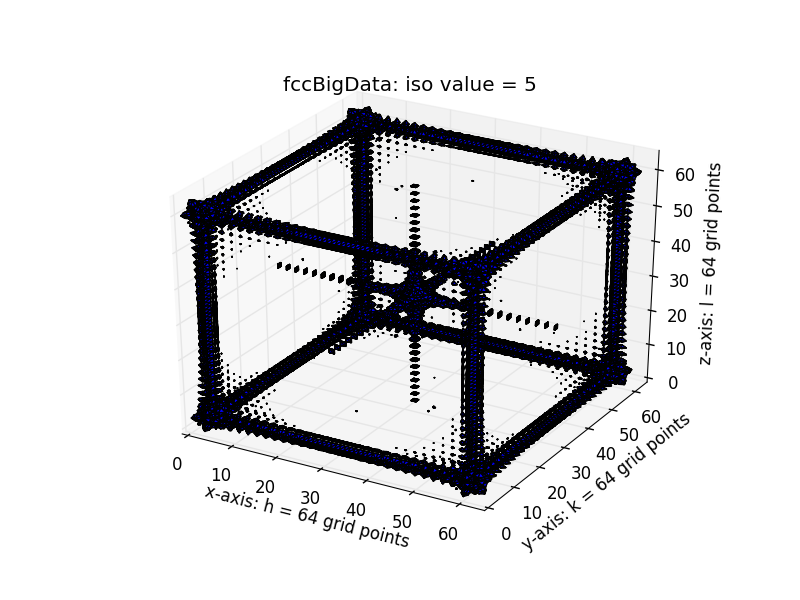
\includegraphics[width=1.58\textwidth]{pics/fccBigData_isosurf64.png}
    \end{column}
    \hspace*{1.3cm}
    \end{columns}      
    % My comments
    % The scikit-image SciKit (toolkit for SciPy) extends scipy.ndimage to provide a versatile set of image processing routines. It is written in the Python language.
    % This SciKit is developed by the SciPy community. All contributions are most welcome! Please join us on the mailing list (address provided below). 
    % Marching cubes is an algorithm to extract a 2D surface mesh from a 3D volume.    
    % This can be conceptualized as a 3D generalization of isolines on topographical or weather maps. It works by iterating across the volume, looking for regions which cross the level of interest. If such regions are found, triangulations are generated and added to an output mesh. The final result is a set of vertices and a set of triangular faces.     
\end{frame}

\begin{frame}[fragile]
\frametitle{NumPy to VTK}
%: Converting your NumPy arrays to VTK arrays and files}
%\begin{columns}
%\begin{column}{0.6\textwidth}

\begin{lstlisting}
from pyevtk.hl import gridToVTK
h=k=l = np.linspace(-1.1, 1.1, num=N, endpoint=True, dtype='float64')
gridToVTK("/viz/vtk/" + filename, h, k, l, pointData = {"pow_spec" : pow_spec})
\end{lstlisting}
%\end{column}
%\begin{column}{0.4\textwidth}
%\end{column}
%\end{columns}
\begin{block}{PyEVTK: a great little package by a Paulo Herrera}
\begin{enumerate}
\item \small \texttt{\$ pip install pyevtk}
\item \small save \textbf{NumPy} arrays straight to different types of \textcolor{red}{VTK XML-based} 
\item \small visualize and process your \textbf{NumPy} arrays with any of the flagship VTK applications such as \textcolor{blue}{ParaView, VisIt, Mayavi}
% file formats (not the old legacy ones), without even needing to have VTK installed in your system, making NumPy the only dependency. This way, you can easily save your NumPy arrays into files that can be visualized and processed with any of the flagship VTK applications such as ParaView, VisIt, Mayavi, while obviously you can easily load said files with VTK and use all the goodies the toolkit offers.
\end{enumerate}
\end{block}
\end{frame}
% # **************************************************************
% # * Apply the high level gridToVTK function to our 3D dataset. *
% # * This example shows how to export a rectilinear grid.       *
% # **************************************************************
%------------------------------------------------
\subsection{Getting started with ParaView} % Sections can be created in order to organize your presentation into discrete blocks, all sections and subsections are automatically printed in the table of contents as an overview of the talk
%------------------------------------------------

%\subsection{Introduction} % A subsection can be created just before a set of slides with a common theme to further break down your presentation into chunks

\begin{frame}
    \frametitle{What is ParaView?}
        \begin{itemize}
            \item ParaView is an \textbf{open-source application} and \textbf{architecture display} and analysis of scientific data sets;
            \item ParaView has been demonstrated to process billions of unstructured cells and to process over a trillion structured cells; 
            \item ParaView's parallel framework has run on over 100,000 processing cores {\tiny (from notebooks to world's largest supercomputers)};
            \item ParaView's \textbf{key features} are:
            \begin{itemize}
                \item An open-source scalable, multi-platform for visualizing \textbf{2D/3D data} {\tiny (excels at traditional scientific vis qualitative 3D rendering)};
                \item An extensible, modular \textbf{architecture} based on open standards {\tiny e.g. Custom apps, plugins, \texttt{Python} scripting, \texttt{ParaViewWeb}, \texttt{Catalyst}} 
                \item Support for distributed computation models to process \\ \textbf{large data sets}; 
                \item An open, extensible, and \textbf{intuitive user interface}.
                % \item A flexible BSD 3-clause license; 
                % \item Commercial maintenance and support
            \end{itemize}
        \end{itemize}
\end{frame}

%------------------------------------------------

\begin{frame}
\frametitle{ParaView: a standard de-facto}
    \begin{itemize}
        \item ParaView is primarily developed and published by Kitware Inc. 
              \begin{itemize}
              \item A flexible BSD 3-clause license;
              \item Commercial maintenance and support; 
              \end{itemize}
        \item ParaView is used by many academic, government, and commercial institutions all over the world;
        \item ParaView is downloaded roughly 100,000 times every year; 
        \item ParaView also won the HPCwire Readers' Choice Award and HPCwire Editors' Choice Award for Best HPC Visualization Product or Technology. 
    \end{itemize}    
     
\includegraphics[width=0.2\textwidth]{pics/ECA_Vis}
     \vspace*{1cm}
\end{frame}

%------------------------------------------------

\begin{frame}
\frametitle{ParaView: The architecture}
The application most people associate with ParaView is really just a small client application built on top of a {\bf tall stack} of libraries that provide ParaView with its functionality.
    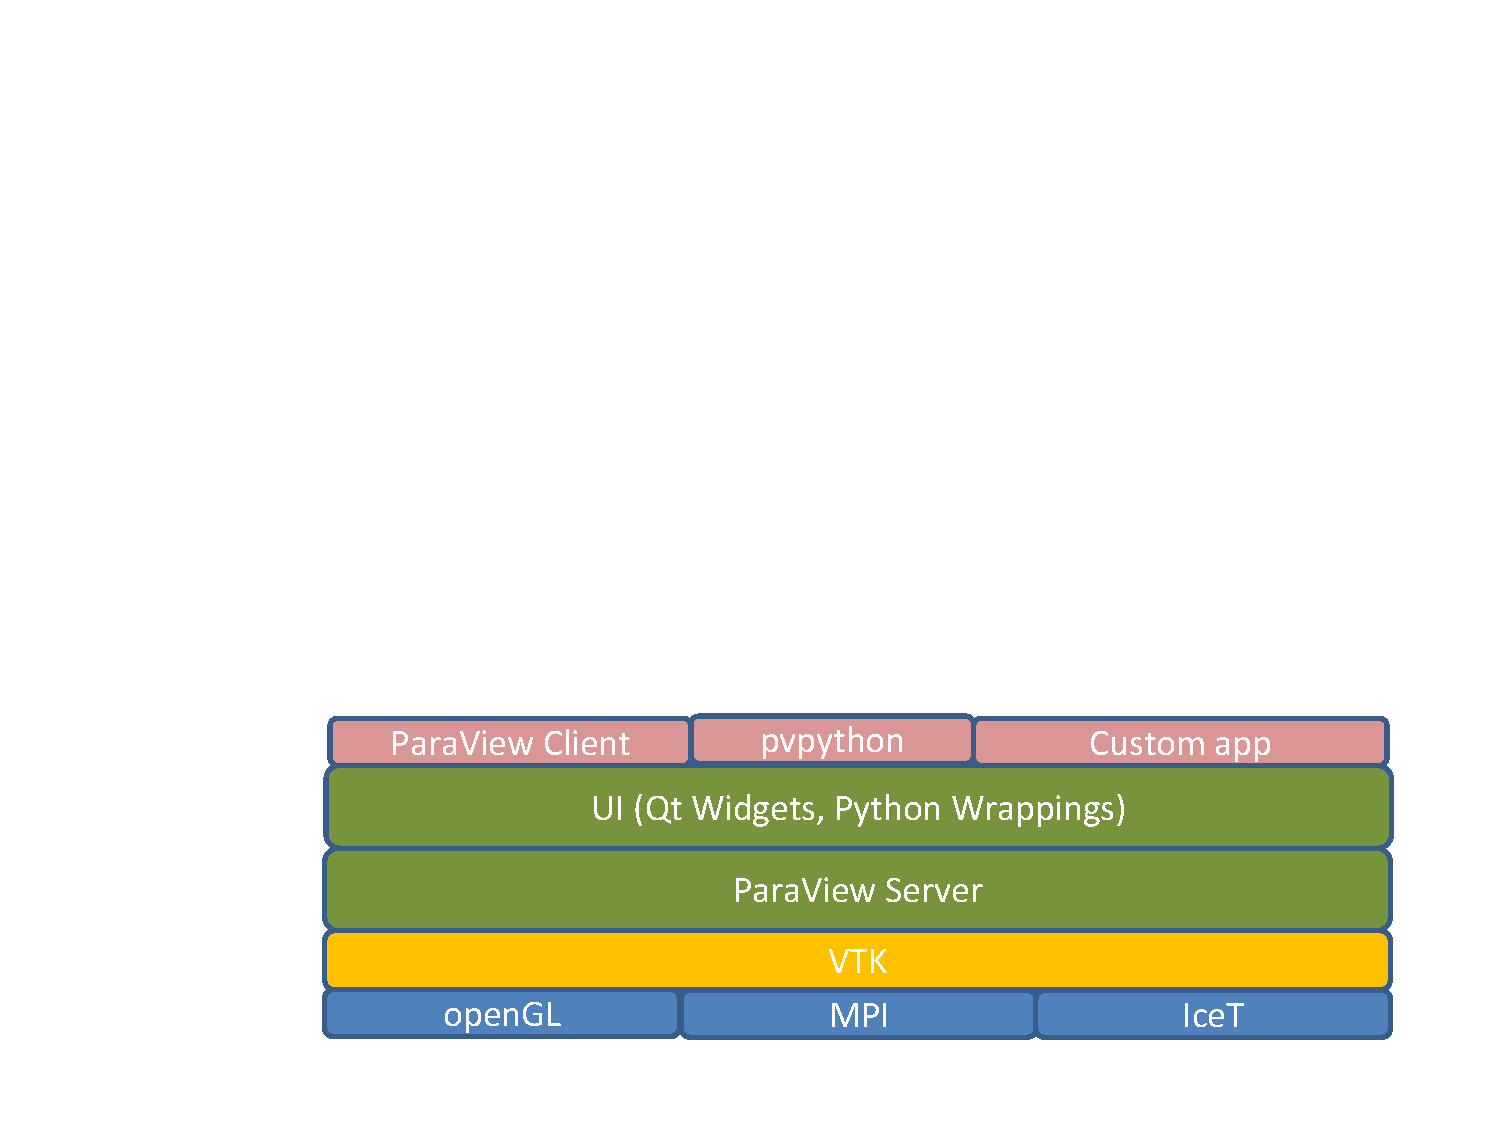
\includegraphics[width=1.\textwidth]{pics/paraview_arch}   
\end{frame}

%------------------------------------------------

\begin{frame}
\frametitle{ParaView: The big picture}
The application most people associate with ParaView is really just a small client application built on top of a {\bf tall stack} of libraries that provide ParaView with its functionality.
      \begin{block}{Full Stack}
        \begin{itemize}
            \item \small ParaView comes with a \textbf{\texttt{pvpython}} application that allows you to automate the visualization and post-processing with \textbf{\texttt{Python}} scripting;
            \item \small ParaView Server library \textbf{\texttt{pvserver}} provides the abstraction layer necessary for running parallel, interactive visualization. It relieves the client application from most of the issues concerning if and how ParaView is running in parallel;
            \item \small The \textbf{Visualization Toolikit} (VTK) provides the basic visualization and rendering algorithms $\Rightarrow$~ \textbf{Data-Flow Paradigm}
        \end{itemize}
    \end{block}
\end{frame}

%------------------------------------------------
%\subsection{Graphical User Interface}

\begin{frame}
\frametitle{ParaView: Loading, filtering and rendering}
\begin{columns}
 \begin{column}{.2\textwidth}
    \begin{block}{GUI elements}<1-7>
          \begin{itemize}
          \item <1-| alert@2> \small Menu\,\tikz[na] \coordinate (Gmenu);
          \item <1-| alert@3> \small Toolbars\,\tikz[na] \coordinate (Gtoolbars);
          \item <1-| alert@4> \small Pipeline\,\tikz[na] \coordinate (Gpipeline);
          \item <1-| alert@5> \small Inspector\,\tikz[na] \coordinate (Ginspector);
          \item <1-| alert@6> \small Help\,\tikz[na] \coordinate (Ghelp);
          \item <1-| alert@7> \small Views\,\tikz[na] \coordinate (Gviews);
      \end{itemize}
    \end{block}
 \end{column}
 \begin{column}{.8\textwidth}     
   \begin{tikzpicture}[remember picture,overlay]
  	\node[anchor=south east,inner sep=2.5pt] at ($(current  page.south 	east)+(0cm,1.5cm)$) {
    	 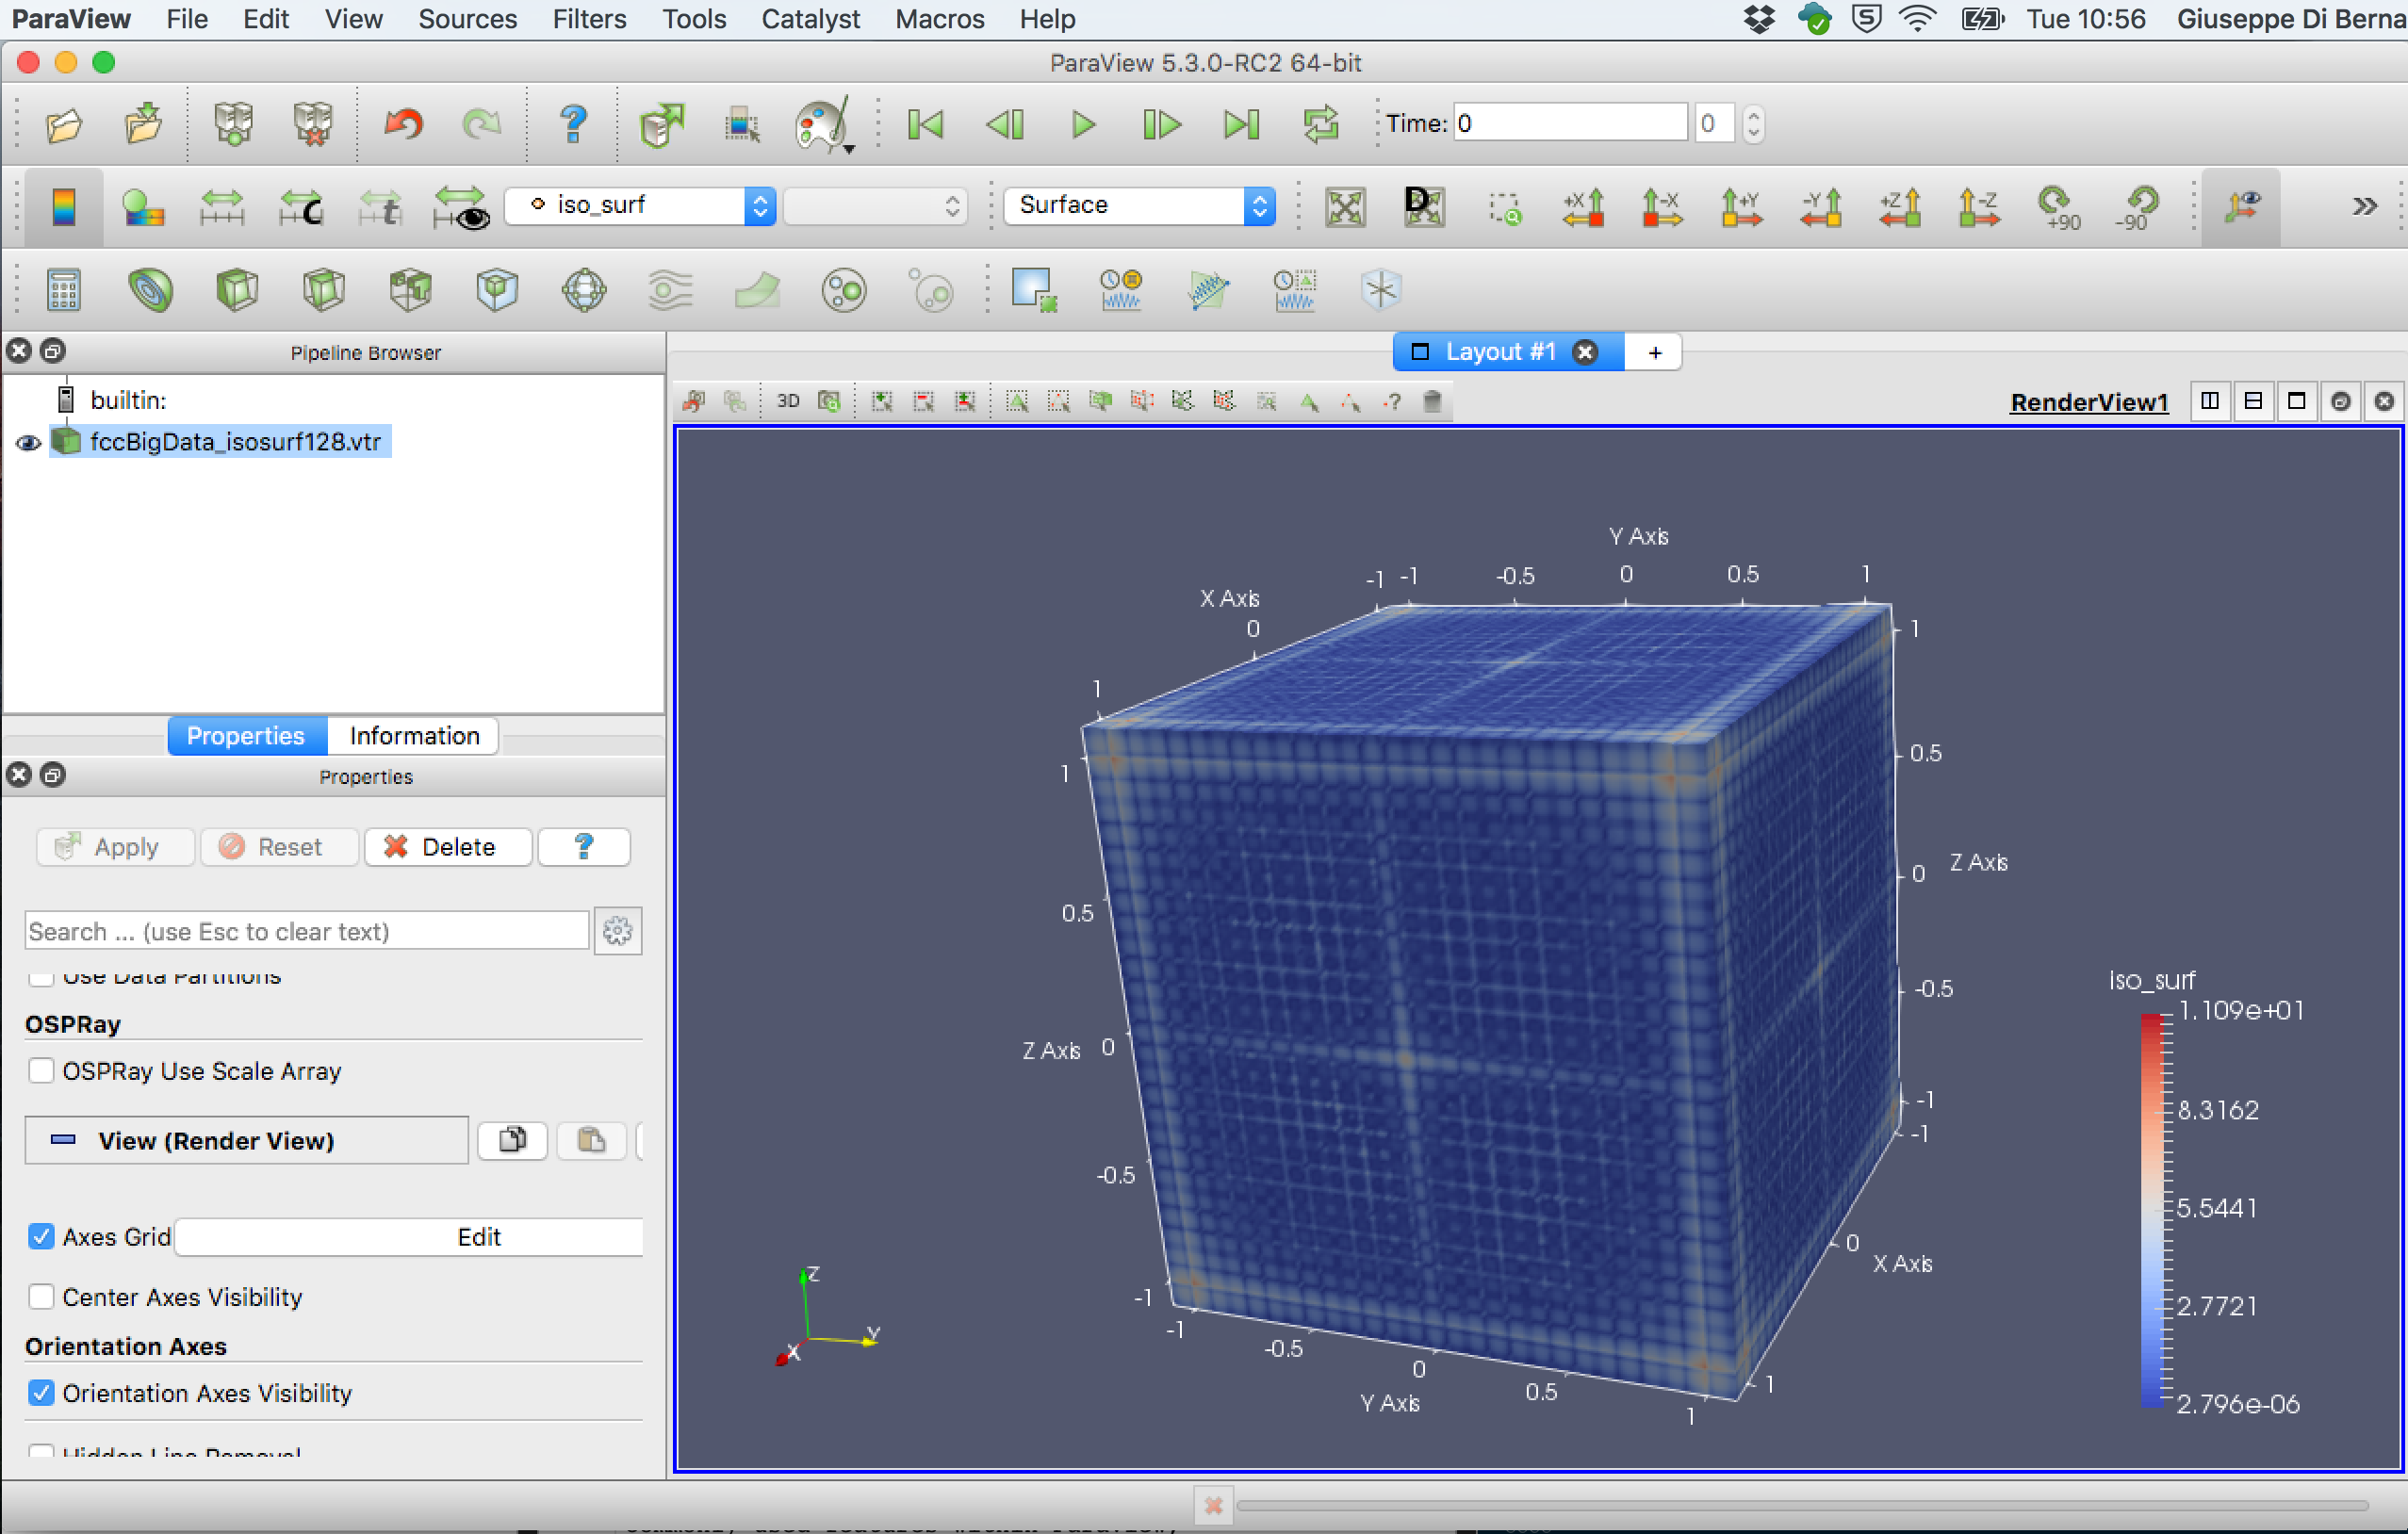
\includegraphics[width=1.08\textwidth]{pics/GUI_elements_2}
    	 %\caption{User Interface}
  		};
        \path (.3,2.7+0.5) coordinate (Menu);
        \path (.3,2.1+0.5) coordinate (Toolbars);
        \path (.3,1.5+0.5) coordinate (Pipeline);
        \path (1.4,.5) coordinate (Inspector);
        \path (2.2,.05) coordinate (Help);
        \path (3.5,-1.8+0.5) coordinate (Views);
   \end{tikzpicture}
 \end{column}
\end{columns}

\begin{tikzpicture}[overlay]
        \draw<2> [thin, red,opacity=.8, fill=red,fill opacity=0.3](Menu) circle (0pt);
        \path<2>[->,>=latex', red, shorten >=4pt, opacity=.6] (Gmenu) edge [out=0, in=130] (Menu);

        \draw<3> [thin, red,opacity=.8, fill=red,fill opacity=0.3](Toolbars) circle (0pt);
        \path<3>[->, >=latex', red, shorten >=4pt, opacity=.6] (Gtoolbars) edge [out=0, in=150] (Toolbars);

        \draw<4> [thin, red,opacity=.8, fill=red,fill opacity=0.3](Pipeline) circle (0pt);
        \path<4>[->,>=latex',red, shorten >=4pt, opacity=.6] (Gpipeline) edge [out=0, in=200] (Pipeline);
        
        \draw<5> [thin, red,opacity=.8, fill=red,fill opacity=0.3](Inspector) circle (0pt);
        \path<5>[->,>=latex',red, shorten >=4pt, opacity=.6] (Ginspector) edge [out=0, in=200] (Inspector);
        
        \draw<6> [thin, red,opacity=.8, fill=red,fill opacity=0.3](Help) circle (0pt);
        \path<6>[->,>=latex',red, shorten >=4pt, opacity=.6] (Ghelp) edge [out=0, in=200] (Help);
        
        \draw<7> [thin, red,opacity=.8, fill=red,fill opacity=0.3](Views) circle (0pt);
        \path<7>[->,>=latex',red, shorten >=4pt, opacity=.6] (Gviews) edge [out=0, in=200] (Views);

\end{tikzpicture}
\end{frame}
%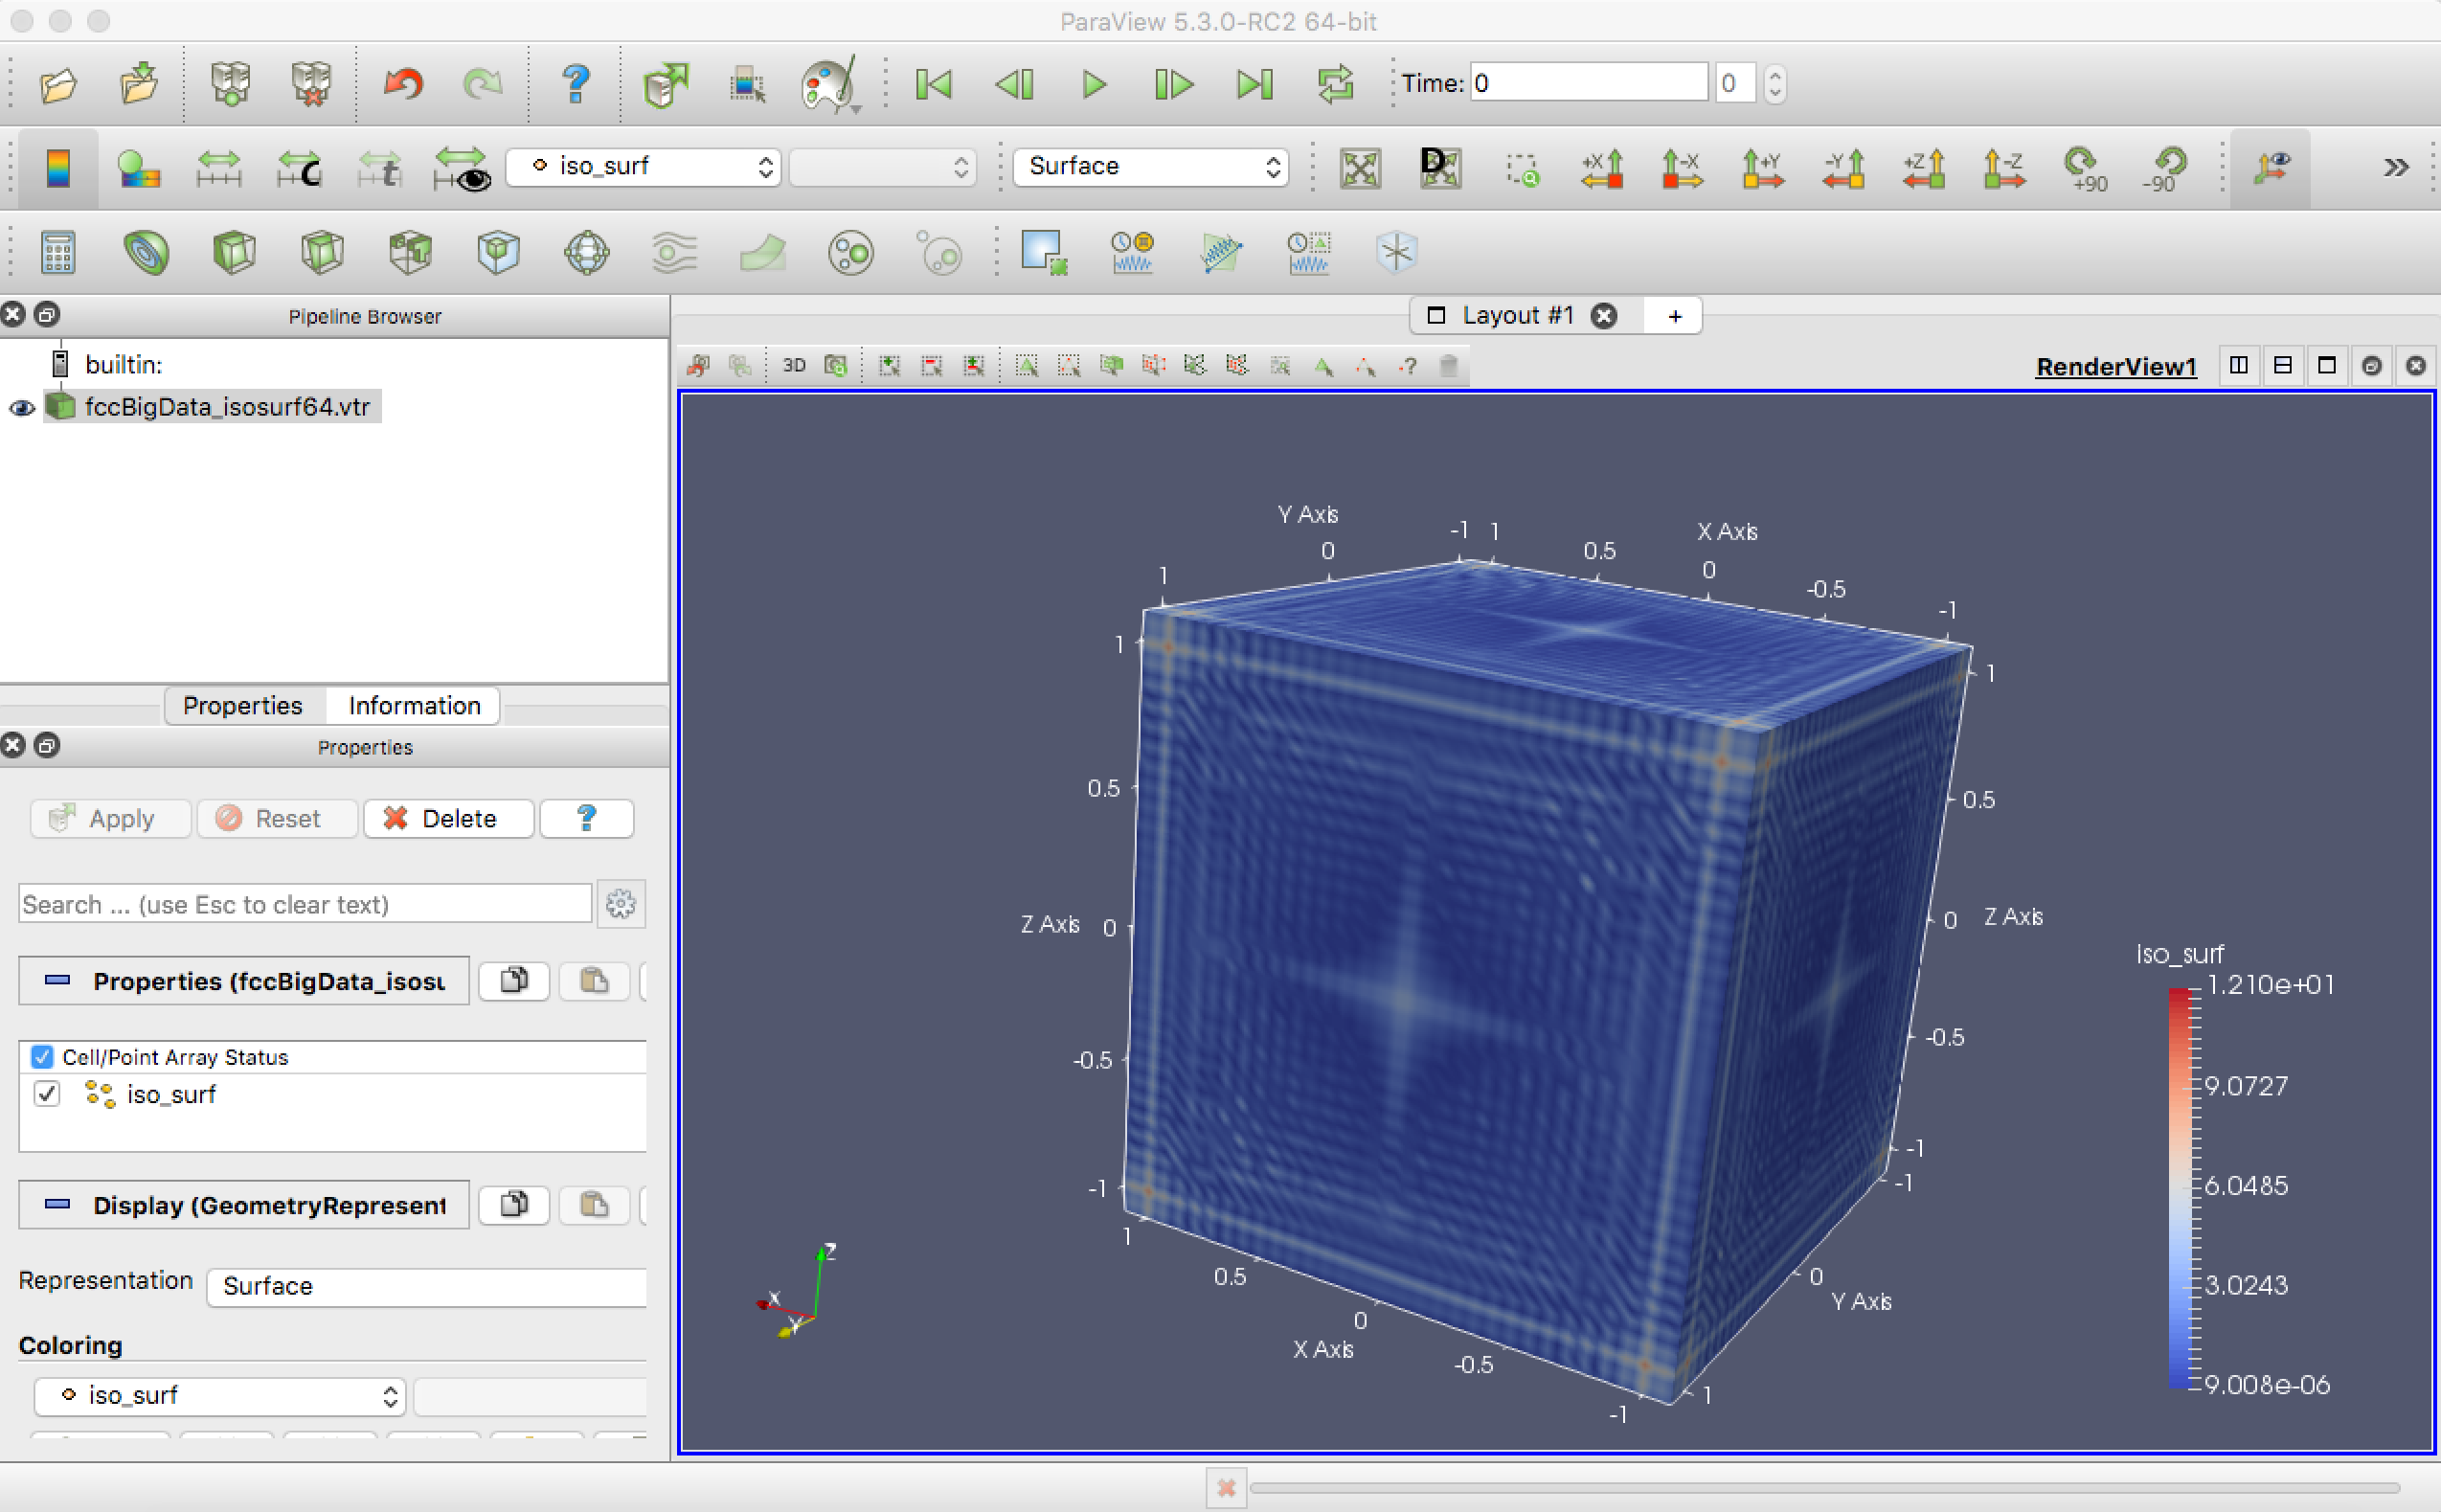
\includegraphics[width=.88\textwidth]{pics/GUI_elements}
%------------------------------------------------

\begin{frame}
\frametitle{GUI elements definition}
    \begin{enumerate}
        \item {\bf Menu Bar}: allows you to access the majority of features; 
        \item {\bf Toolbars}: provide quick access to the most commonly used features within ParaView; 
        \item {\bf Pipeline Browser}: ParaView manages the reading and iterating of  data with a pipeline. A convenient list of pipeline objects with an indentation style that shows the pipeline structure; 
        \item {\bf Properties Panel}: to view and change the parameters of the current pipeline object. The properties are by default coupled with an information tab that shows a basic summary of the data produced by the pipeline object; 
        \item {\bf 3D View}: to present the data so that you may view,\\ interact with, and explore your data.
    \end{enumerate}
\end{frame}

%------------------------------------------------

\begin{frame}
\frametitle{Filters Menu}
    \begin{columns}[c] % The "c" option specifies centered  vertical alignment while the "t" option is used for top vertical alignment
        \column{.5\textwidth} % Left column and width
        \textit{...some of them}
        \begin{enumerate}
            \item {\bf Calculator}: evaluates a user-defined expression on a {\it per-point} or {\it per-cell} basis
            \item {\bf Contour}: extracts the points, curves, or surfaces where a scalar field is equal to a user-defined value. This surface is often also called {\it iso-surface}
\item {\bf Threshold}: extracts cells that lie within a specified range of a scalar-field
% \item Extract Subset
% \item Glyph
% \item Stream Traces
% \item Warp By Vector
% \item Group Datasets
% \item Extract Group 
        \end{enumerate}
        \column{.5\textwidth} % Right column and width
        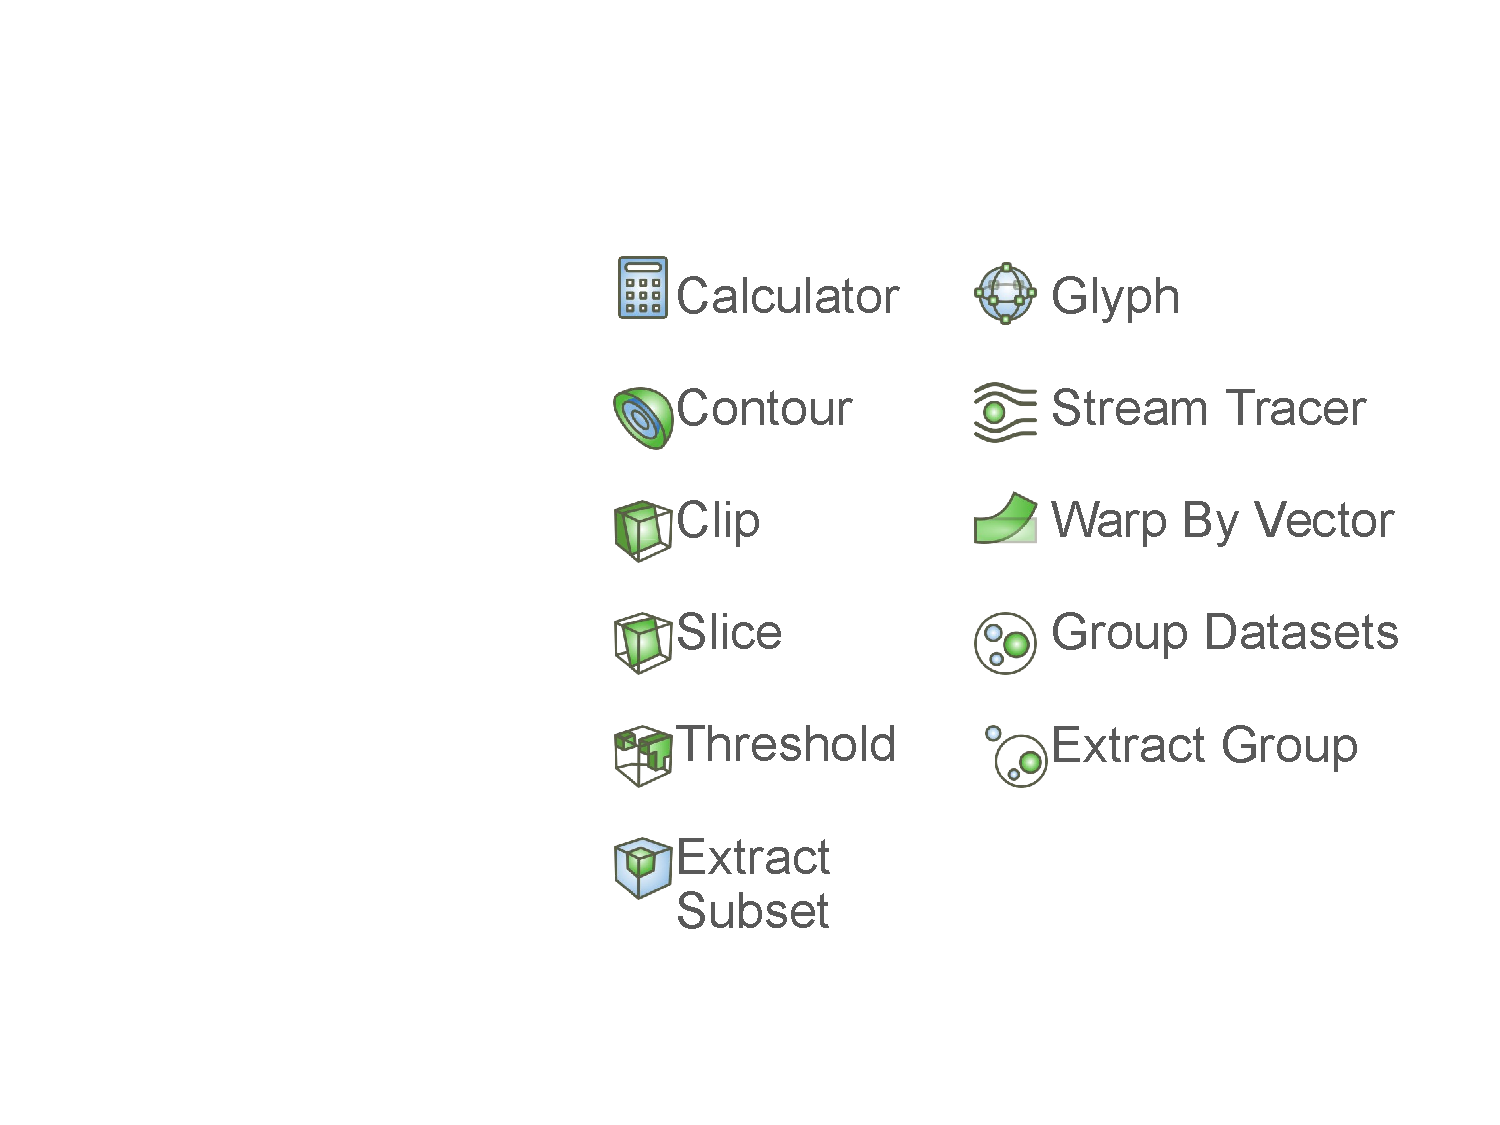
\includegraphics[width=.9999\textwidth]{pics/Filters}
    \end{columns}
\end{frame}

%------------------------------------------------

\begin{frame}
\frametitle{Other Filters}
\begin{columns}[c] % The "c" option specifies centered vertical alignment while the "t" option is used for top vertical alignment

\column{.5\textwidth} % Left column and width
\textit{...some of them}
\begin{itemize}
\item Recent
\item AMR (adaptive mesh refinement)
\item CTH 
\item Common (the same list available in the filters toolbars)
\item Cosmology
\end{itemize}

\column{.5\textwidth} % Right column and width
\begin{itemize}
\item {\bf Data Analysis}: quantitative values from the data
\item Material Analysis
\item {\bf Statistics}: descriptive statistics of the data (primarily in tabular form)
\item Temporal
\item Alphabetical
% \item Extract Group 
\end{itemize}
\end{columns}
\end{frame}

%------------------------------------------------

\begin{frame}
\frametitle{ParaView: Multiple views}
\begin{columns}
\column{0.5\textwidth}
\begin{minipage}[c][0.4\textheight][c]{\linewidth}
  \centering
  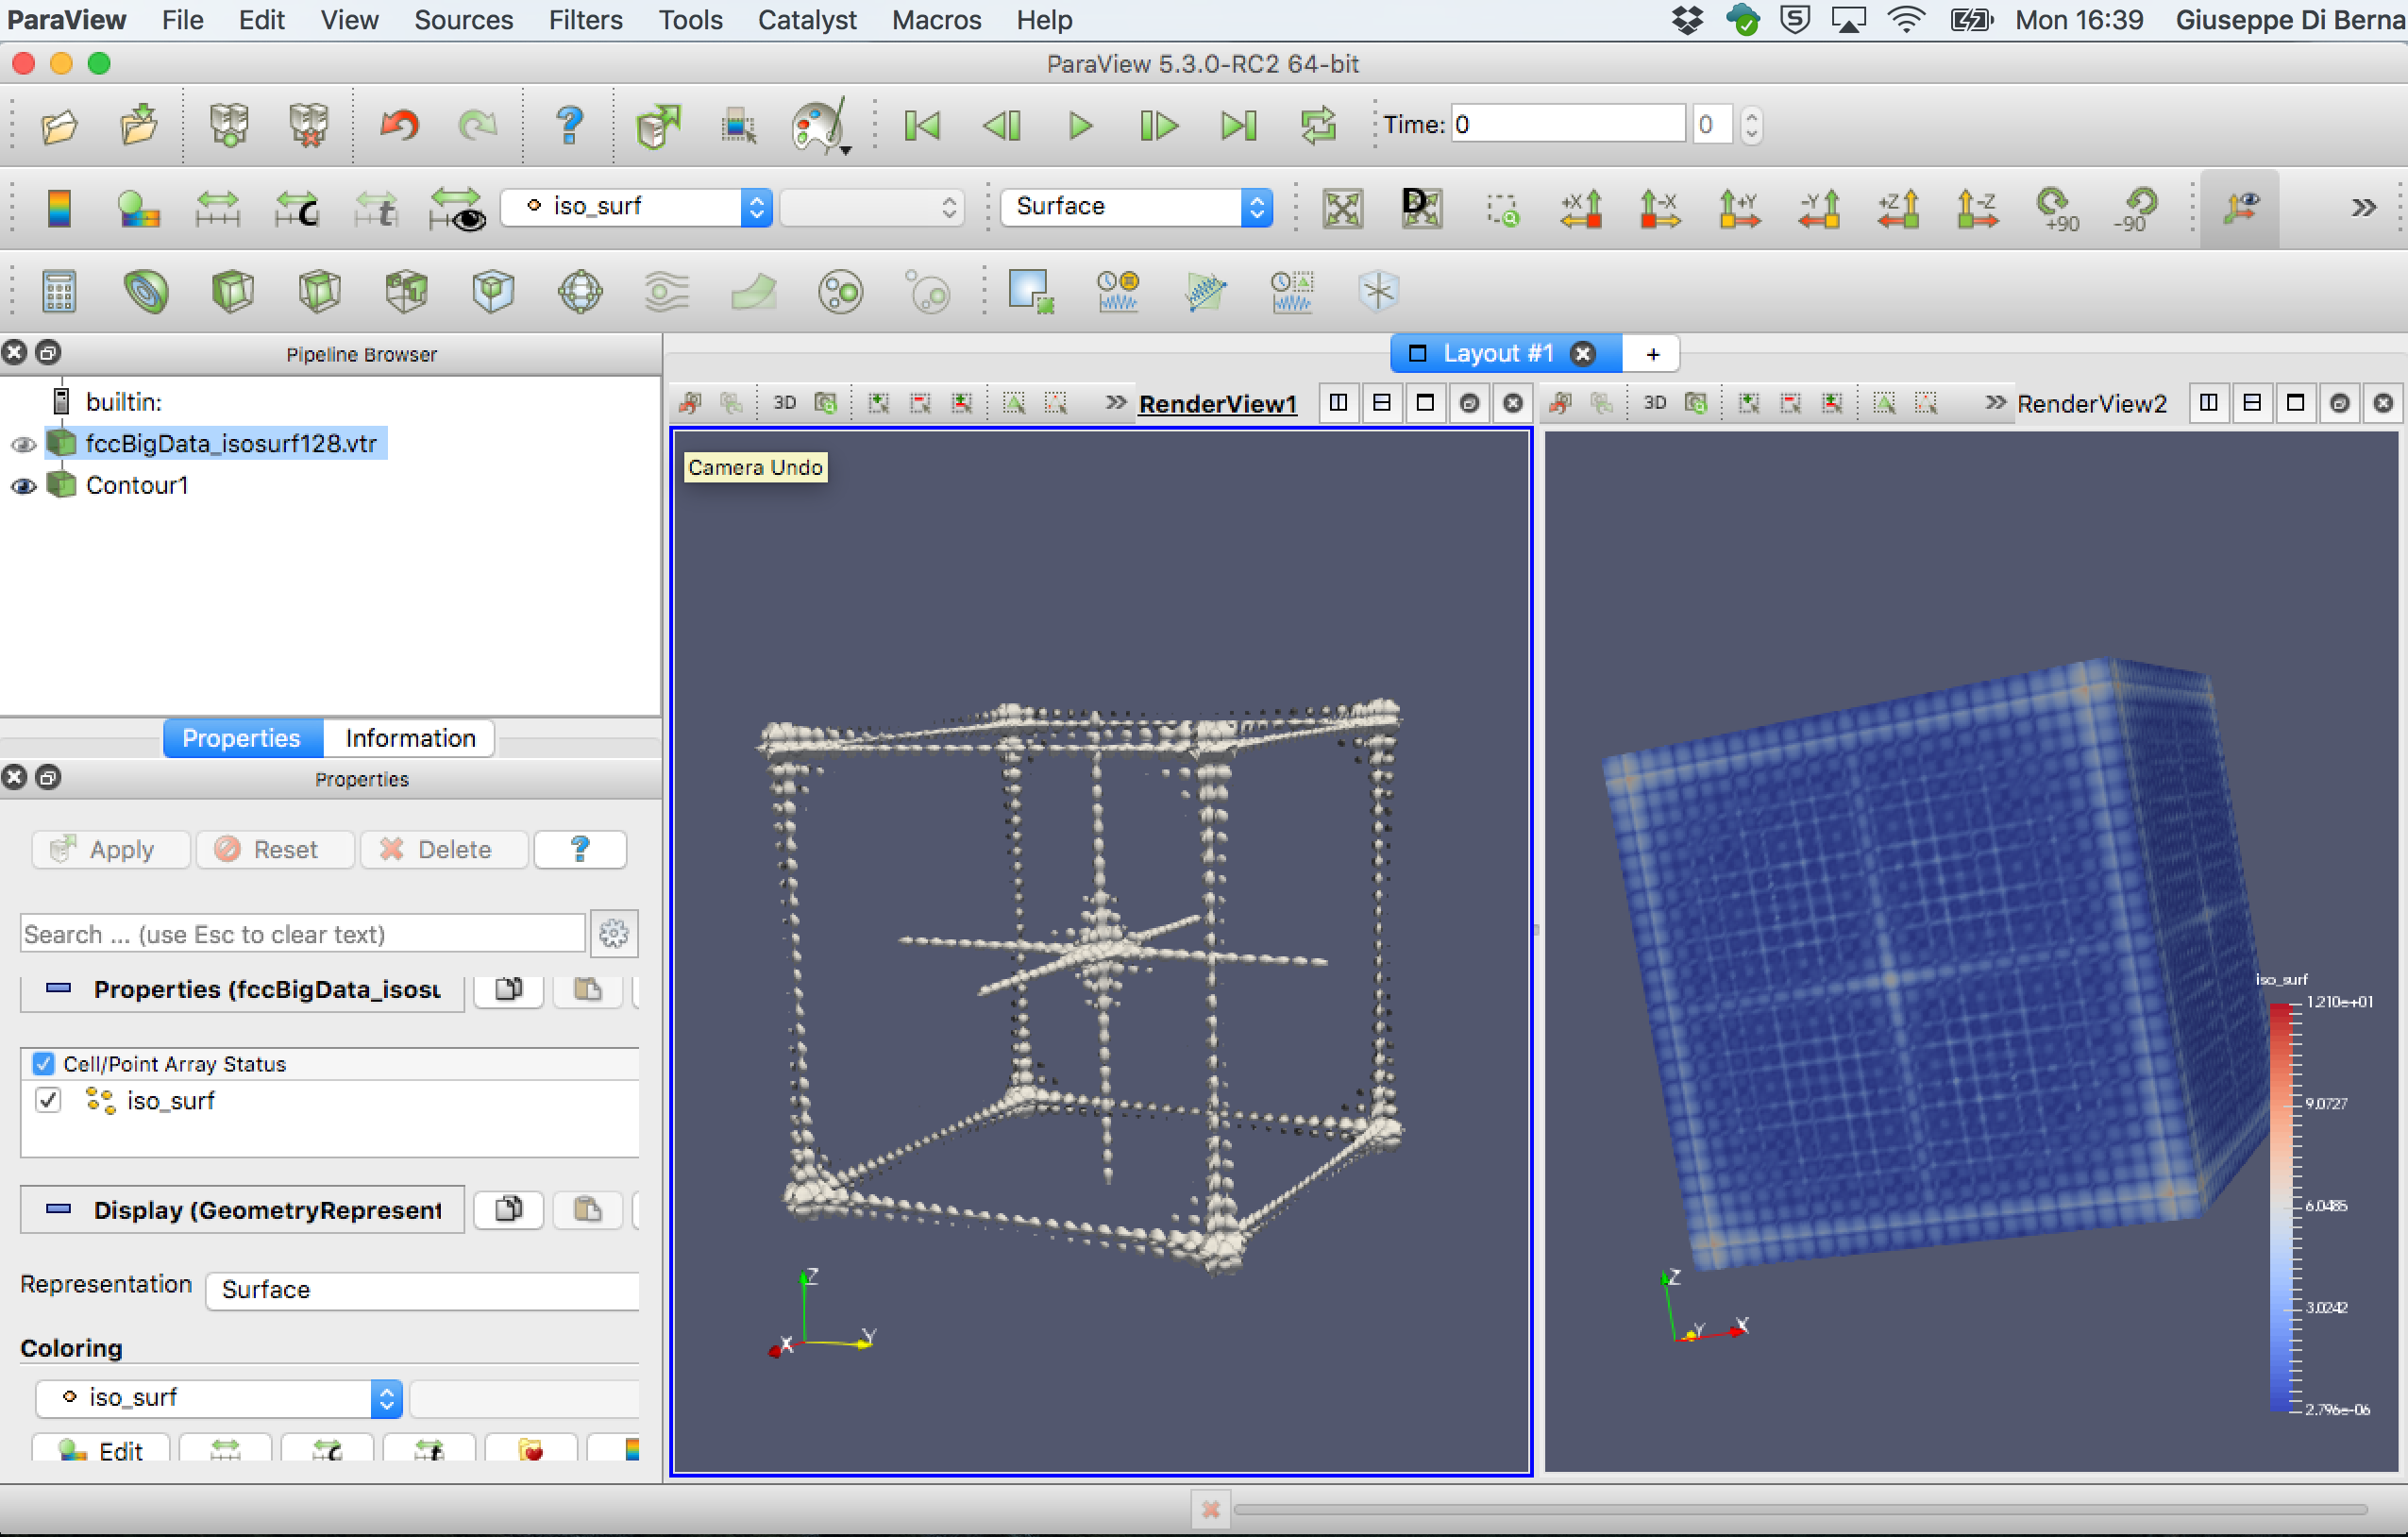
\includegraphics[width=0.8\linewidth]{pics/3d_plus_3d}
\end{minipage}
\begin{minipage}[c][0.4\textheight][c]{\linewidth}
  \centering
  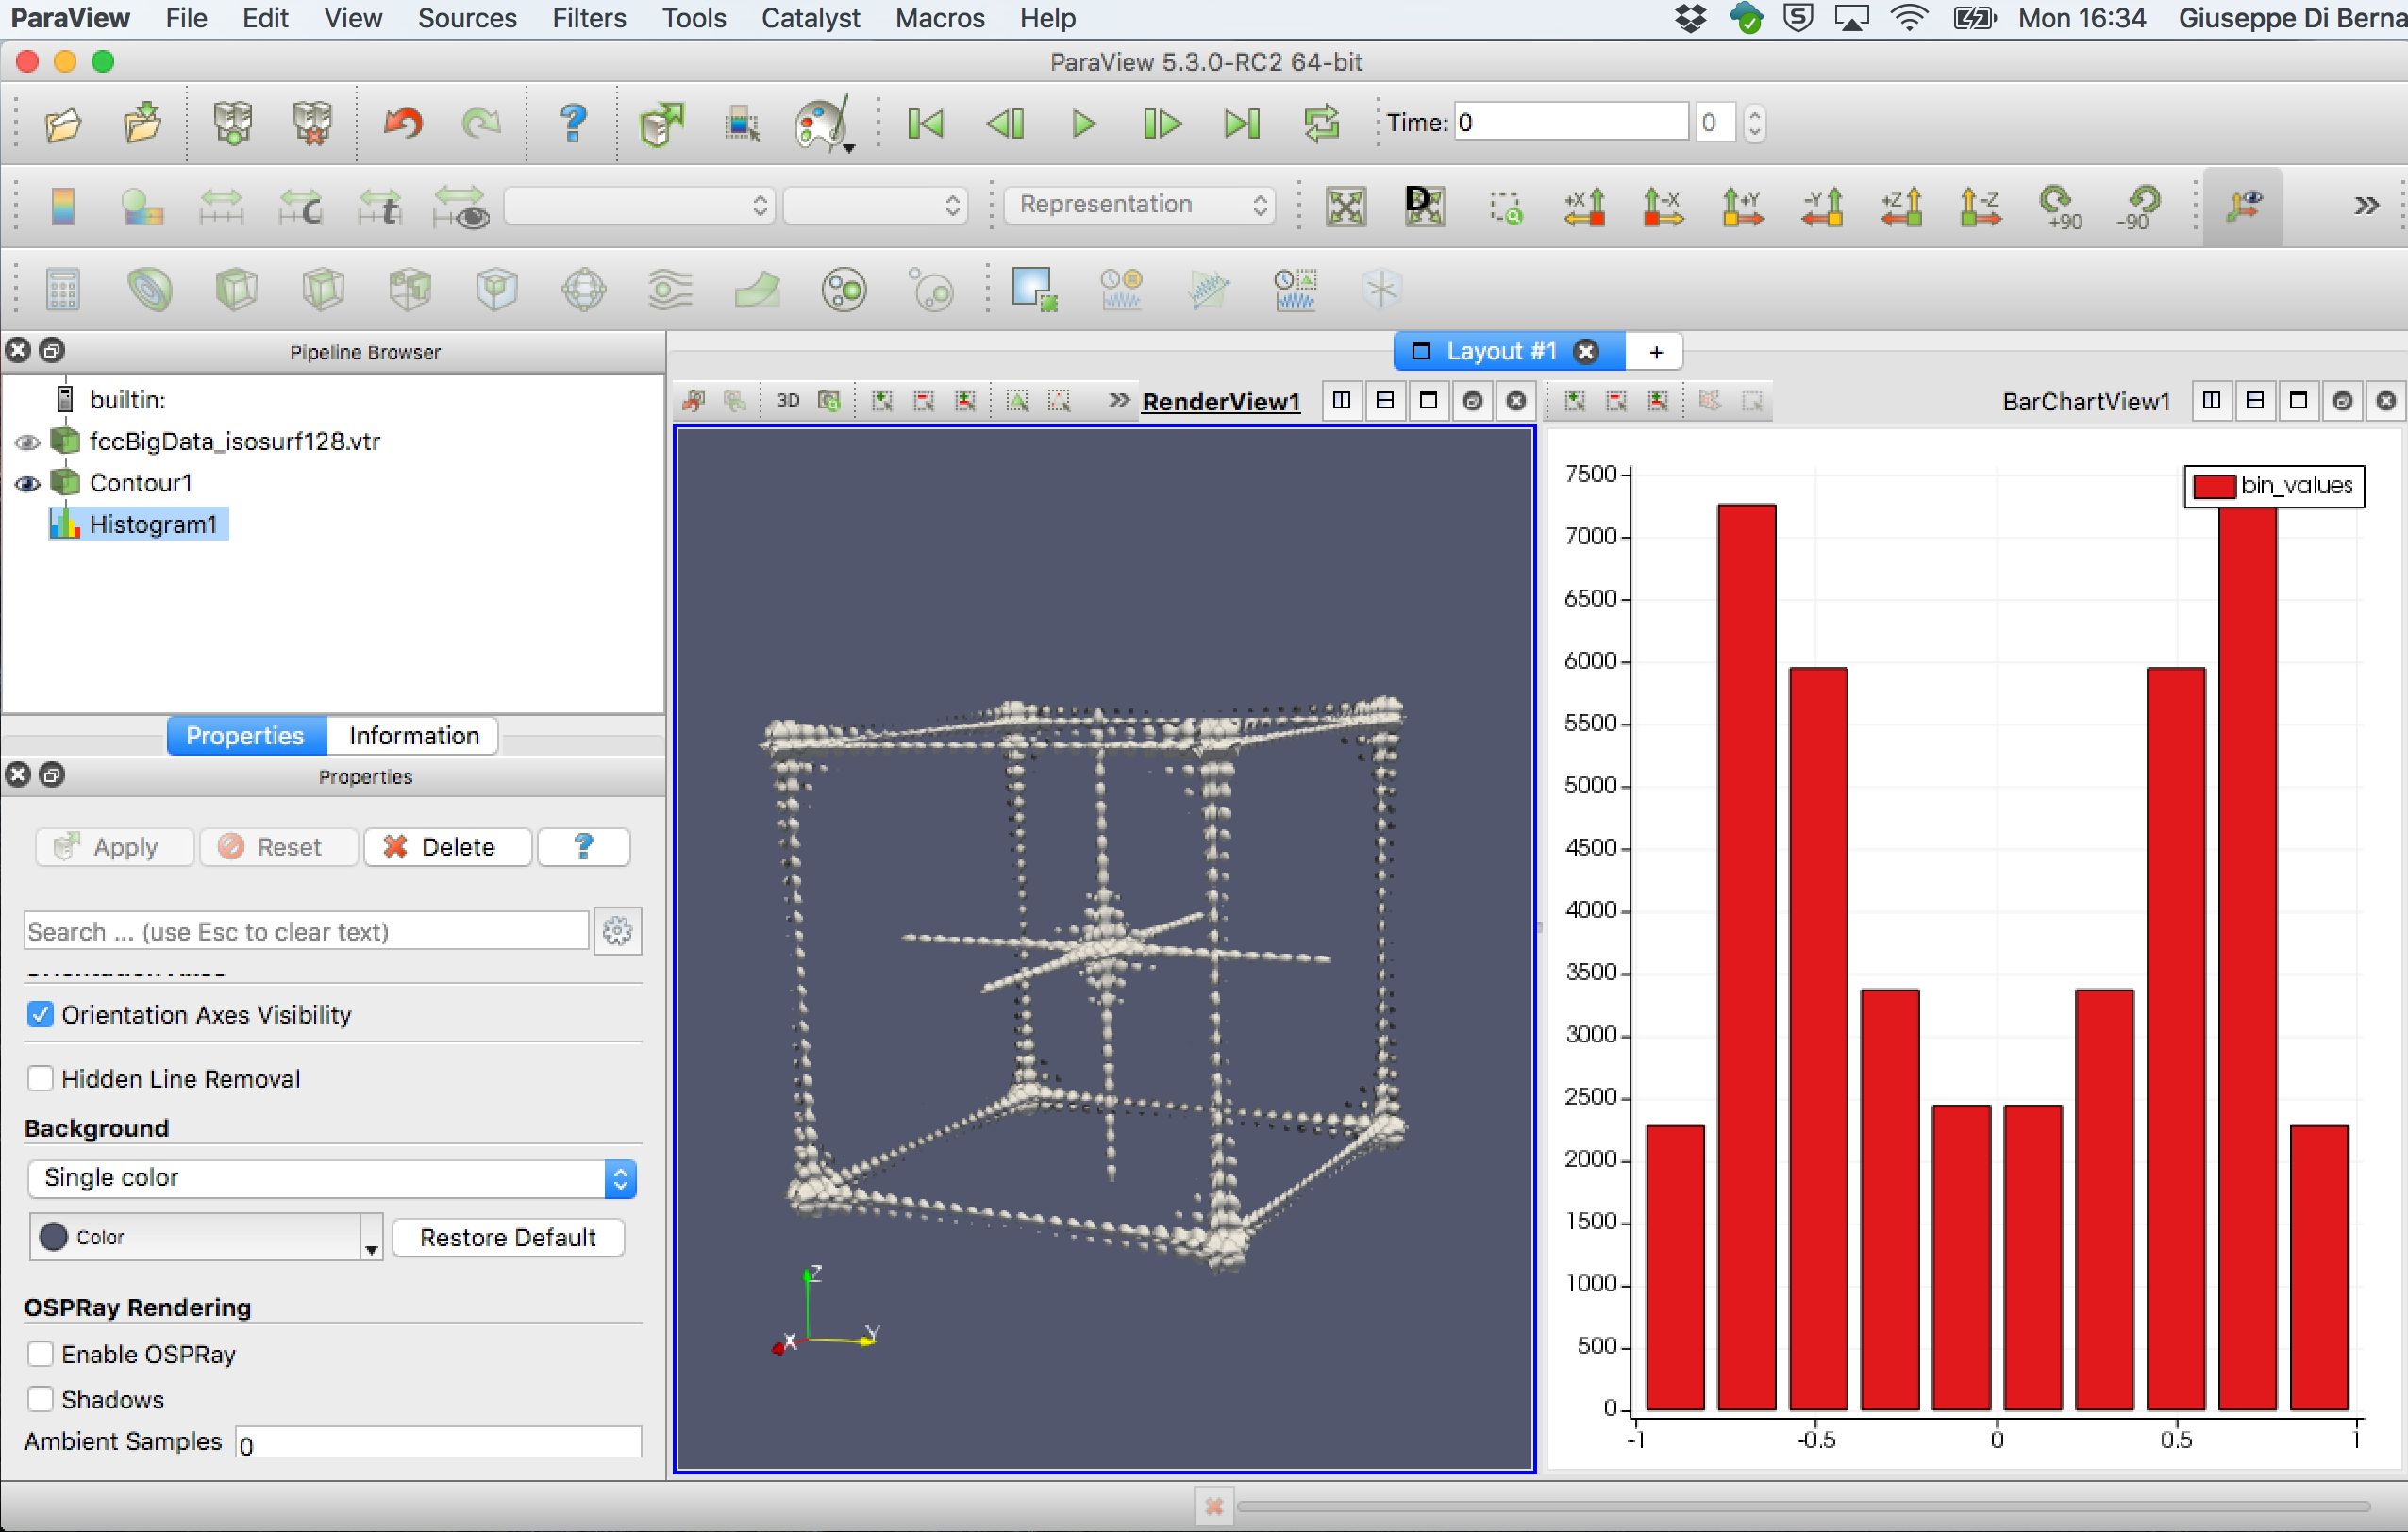
\includegraphics[width=0.8\linewidth]{pics/Multiple_views}
\end{minipage}
\column{0.5\textwidth}
\begin{minipage}[c][0.4\textheight][c]{\linewidth}
  \textbf{Some examples}
  \begin{enumerate}
  \item 3d + 3d
  \item 3d + Histograms
  \item 3d + table
  \end{enumerate}
\end{minipage}
\begin{minipage}[c][0.4\textheight][c]{\linewidth}
  \centering
  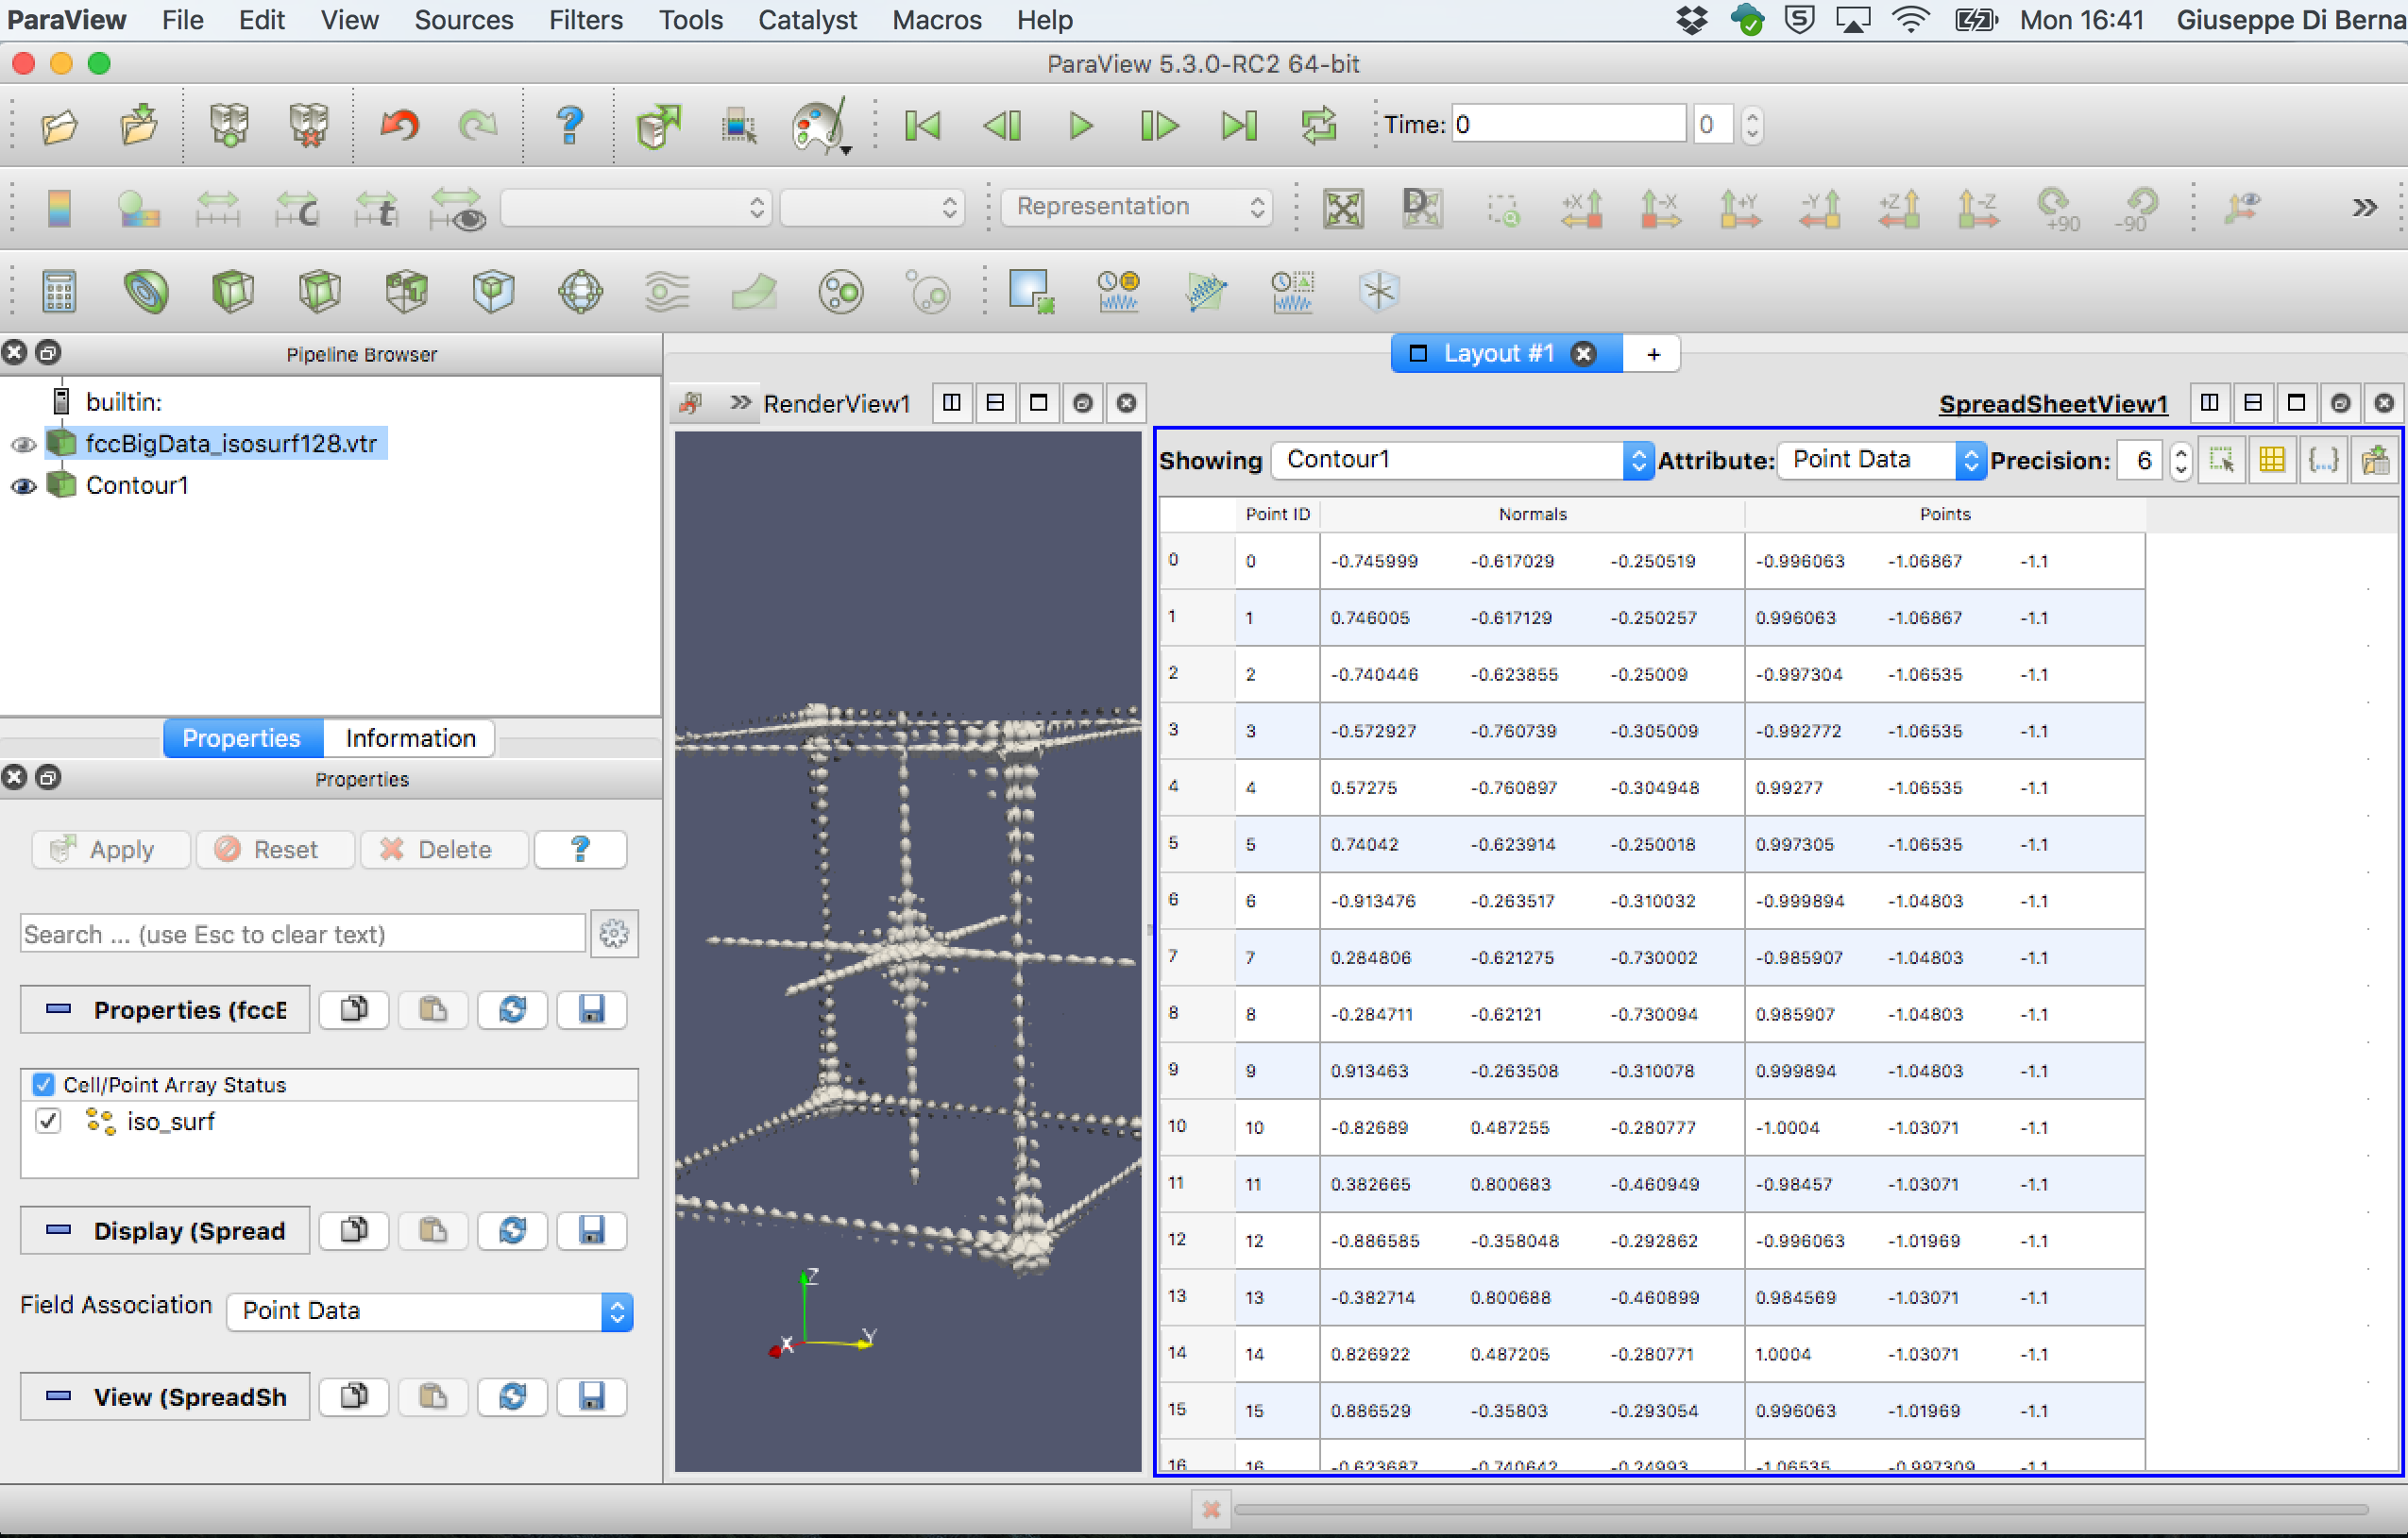
\includegraphics[width=0.8\linewidth]{pics/3d_plus_table}
\end{minipage}
\end{columns}
\end{frame}

%------------------------------------------------
%\section{Data Analytics}
%------------------------------------------------

%------------------------------------------------
%\subsection{Data Types}
%------------------------------------------------
\begin{frame}
ParaView was designed primarily to handle data with spatial representation. Thus the {\bf data types} used in ParaView are meshes 
\frametitle{ParaView: The dataset types (sampling structures)}
    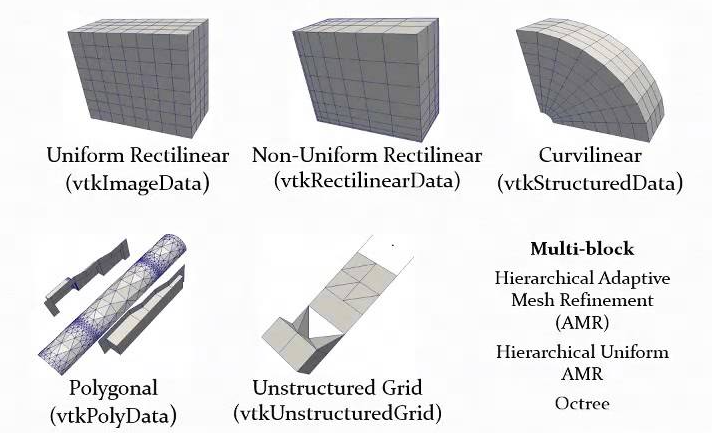
\includegraphics[width=.88\textwidth]{pics/vtk_dataformat}
\end{frame}

\begin{frame}
\frametitle{Data Selection}
The goal of visualization is often to find the importance details within a large body of information. ParaView's selection abstraction is an important simplification of this process. \par Selection is the act of identifying a subset of some dataset. More specifically the subset identifies particular select points, cells, or blocks within any single data set. \par In ParaView, selection can take place at any time, and the program maintains a current selected set that is linked between all views. 
\begin{enumerate}
\item The most direct means to create a selection is via the \texttt{Find Data} dialog 
\includegraphics[width=0.04\linewidth]{pics/Paraview_filter}
\item Another way of creating a selection is to pick elements right inside the 3D view: {\bf rubber-band selection}
\end{enumerate}
\end{frame}

%\subsection{Performing Query-Based Selections}
%------------------------------------------------
\begin{frame}
\frametitle{Query Data by Attribute Values - Find Data dialog}
\begin{columns}
\column{0.5\textwidth}
\begin{minipage}[c][0.4\textheight][c]{\linewidth}
  \centering
  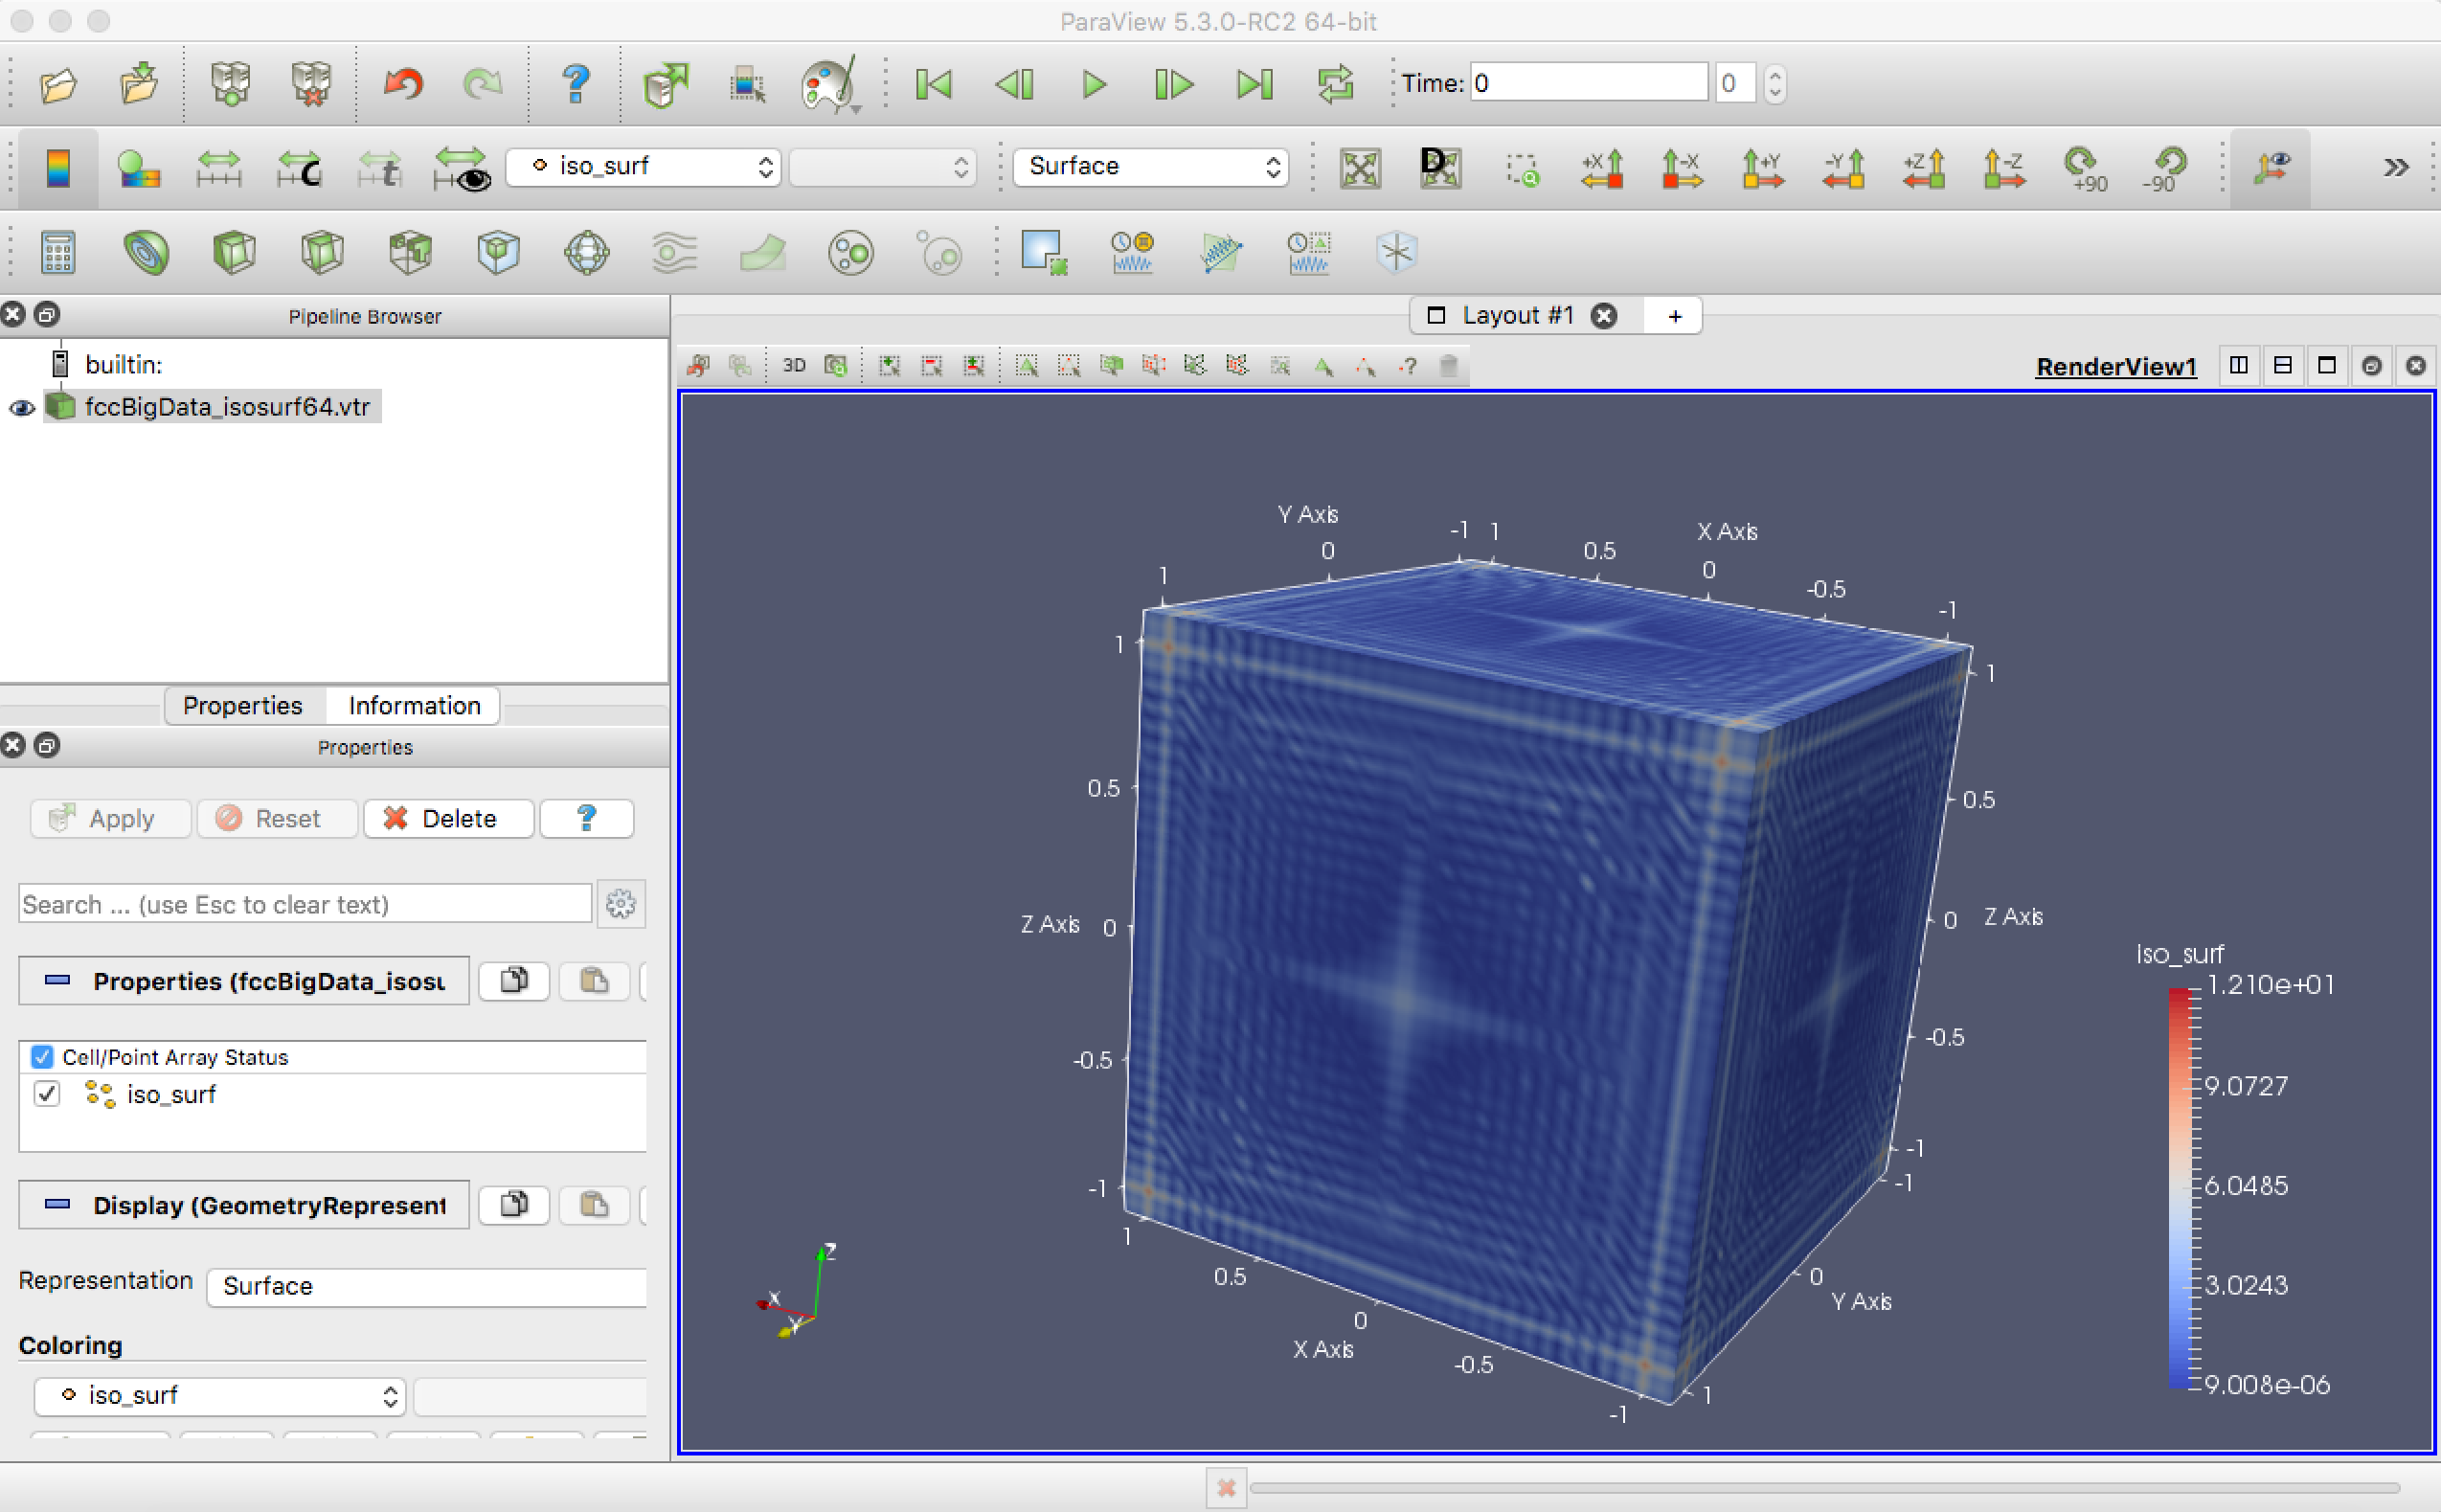
\includegraphics[width=0.8\linewidth]{pics/GUI_elements}
\end{minipage}
\begin{minipage}[c][0.4\textheight][c]{\linewidth}
  \centering
  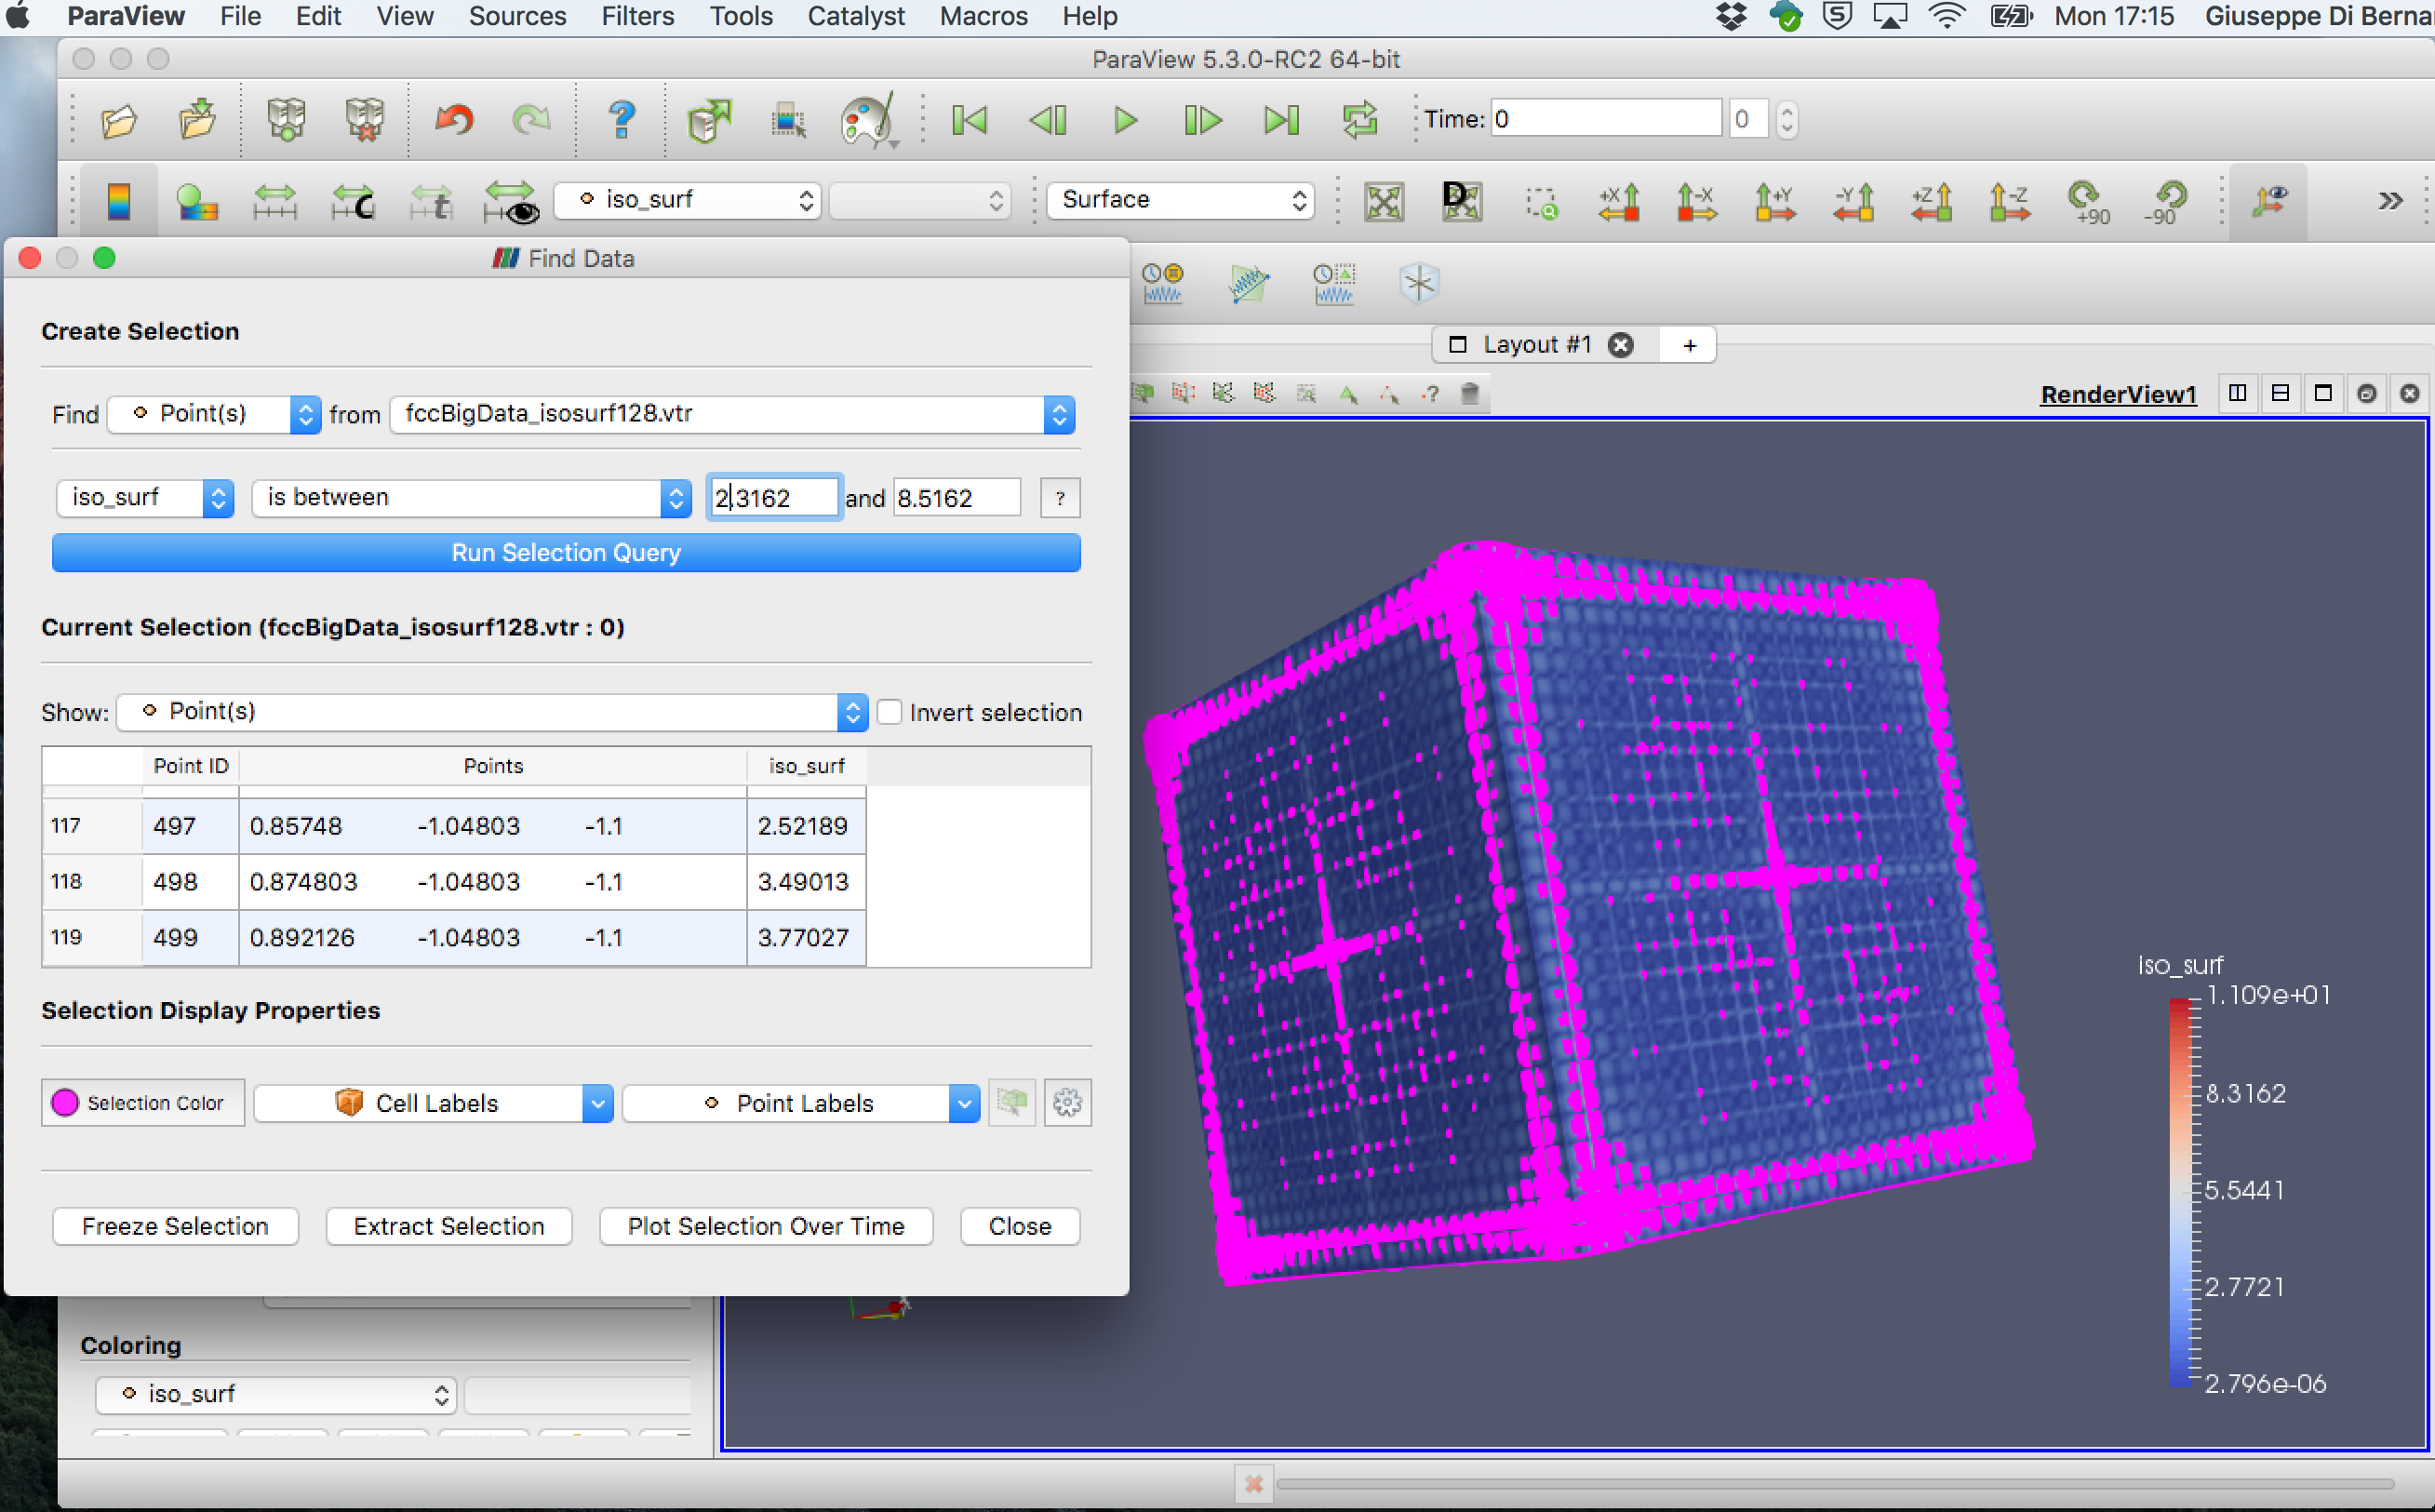
\includegraphics[width=0.8\linewidth]{pics/Data_selection_query.png}
\end{minipage}
\column{0.5\textwidth}
\begin{minipage}[c][0.4\textheight][c]{\linewidth}
  \textbf{Some examples}
  \begin{enumerate}
  \item load, filter and display your volume data 
\includegraphics[width=0.07\linewidth]{pics/load_logo} ~
  
\includegraphics[width=0.08\linewidth]{pics/contour_logo} ~ 
\includegraphics[width=0.2\linewidth]{pics/apply_logo}
  \item find data matching your criteria 
\includegraphics[width=0.08\linewidth]{pics/Paraview_filter}
  \item extract selection ({\tt Run Selection Query})
  \end{enumerate}
\end{minipage}
\begin{minipage}[c][0.4\textheight][c]{\linewidth}
  \centering
  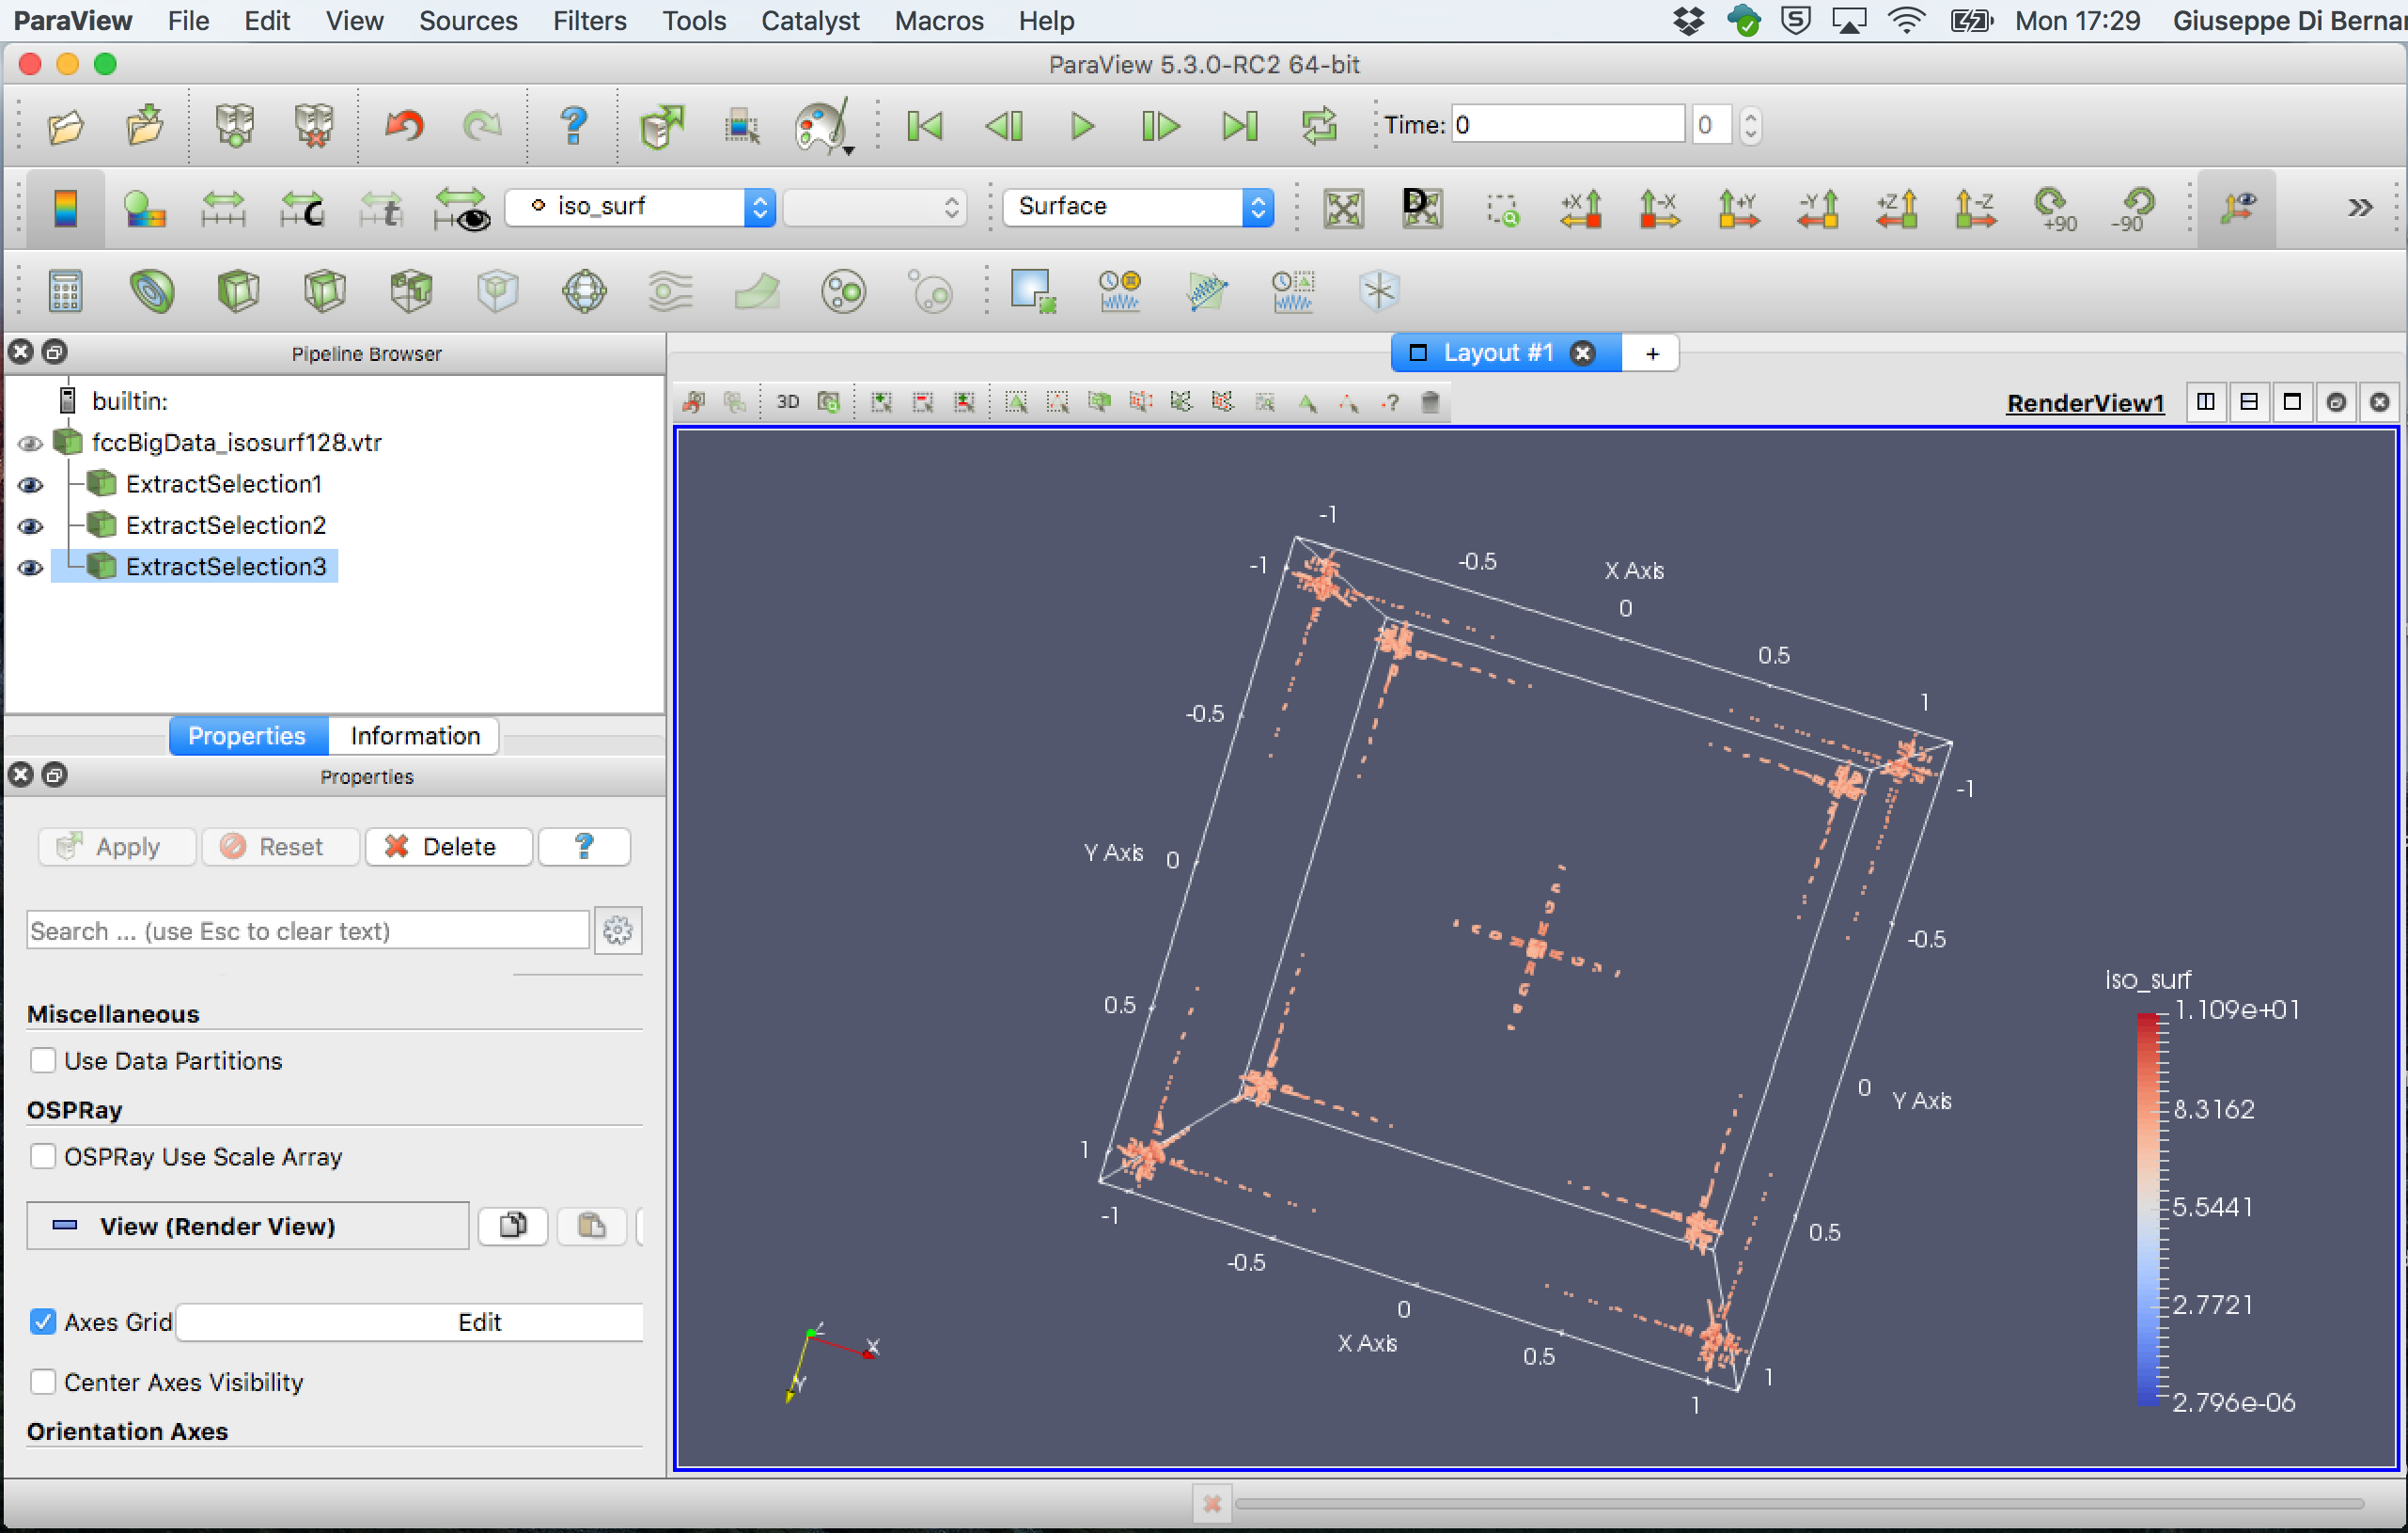
\includegraphics[width=0.8\linewidth]{pics/Data_selection_query2}
\end{minipage}
\end{columns}
\end{frame}

%------------------------------------------------

\begin{frame}
\frametitle{Query Data Spatially - Selection}
    \textit{...by clicking and dragging the mouse in the 3D view}
    \begin{columns}[c] % The "c" option specifies centered  vertical alignment while the "t" option is used for top vertical alignment
        \column{.5\textwidth} % Left column and width
        \begin{itemize}
            \item {\bf Select Cells On (Surface)}: cells that are visible in the view under a rubber band
            \item {\bf Select Points On (Surface)}: points that are visible in the view under a rubber band
            \item {\bf Select Cells Through (Frustum)}: cells that exist under a rubber band
            \item {\bf Select Points Through (Frustum)}
        \end{itemize}
        \column{.5\textwidth} % Right column and width
        \begin{itemize}     
            \item {\bf Select Cells with Polygon}: you draw a polygon
            \item {\bf Select Points with Polygon}
            \item {\bf Select Blocks}: Select blocks in a multiblock dataset
            \item {\bf Int. Select Cells}
            \item {\bf Int. Select Points}
         \end{itemize}
        % 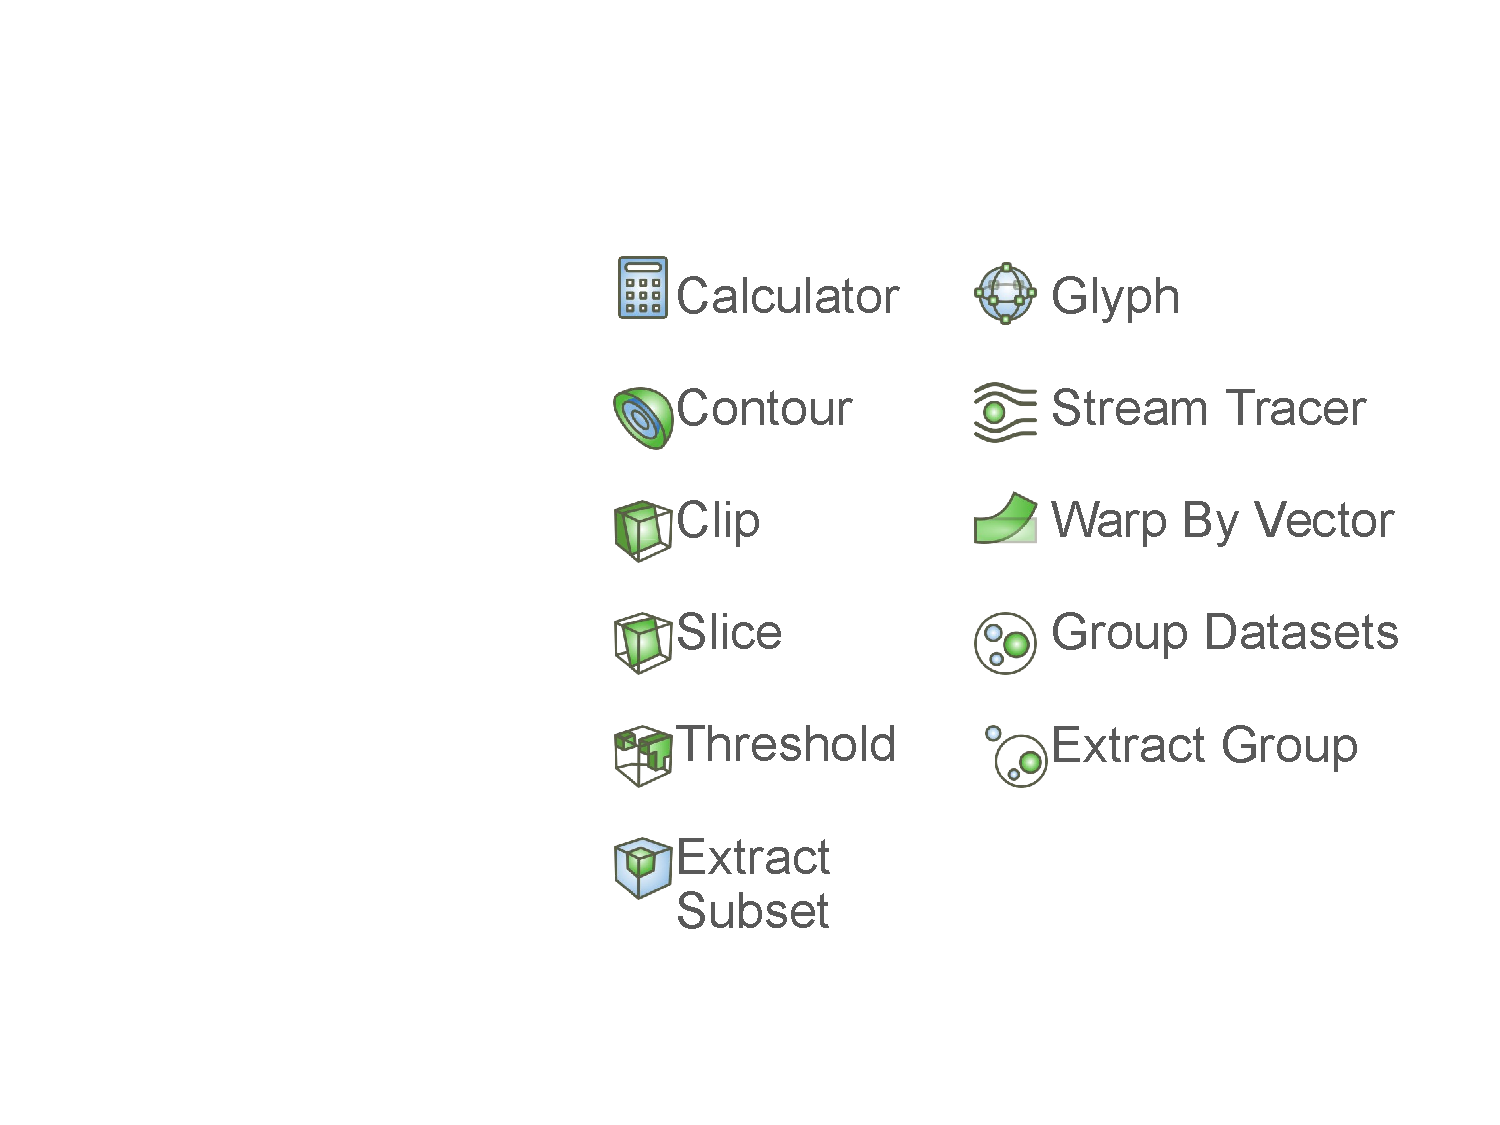
\includegraphics[width=.9999\textwidth]{pics/Filters}
    \end{columns}
\end{frame}

% \begin{frame}
% \frametitle{Table}
% \begin{table}
% \begin{tabular}{l l l}
% \toprule
% \textbf{Treatments} & \textbf{Response 1} & \textbf{Response 2}\\
% \midrule
% Treatment 1 & 0.0003262 & 0.562 \\
% Treatment 2 & 0.0015681 & 0.910 \\
% Treatment 3 & 0.0009271 & 0.296 \\
% \bottomrule
% \end{tabular}
% \caption{Table caption}
% \end{table}
% \end{frame}

%------------------------------------------------

\begin{frame}
\frametitle{Query Data Spatially - Selection}
    \textit{...by clicking and dragging the mouse in the 3D view}
     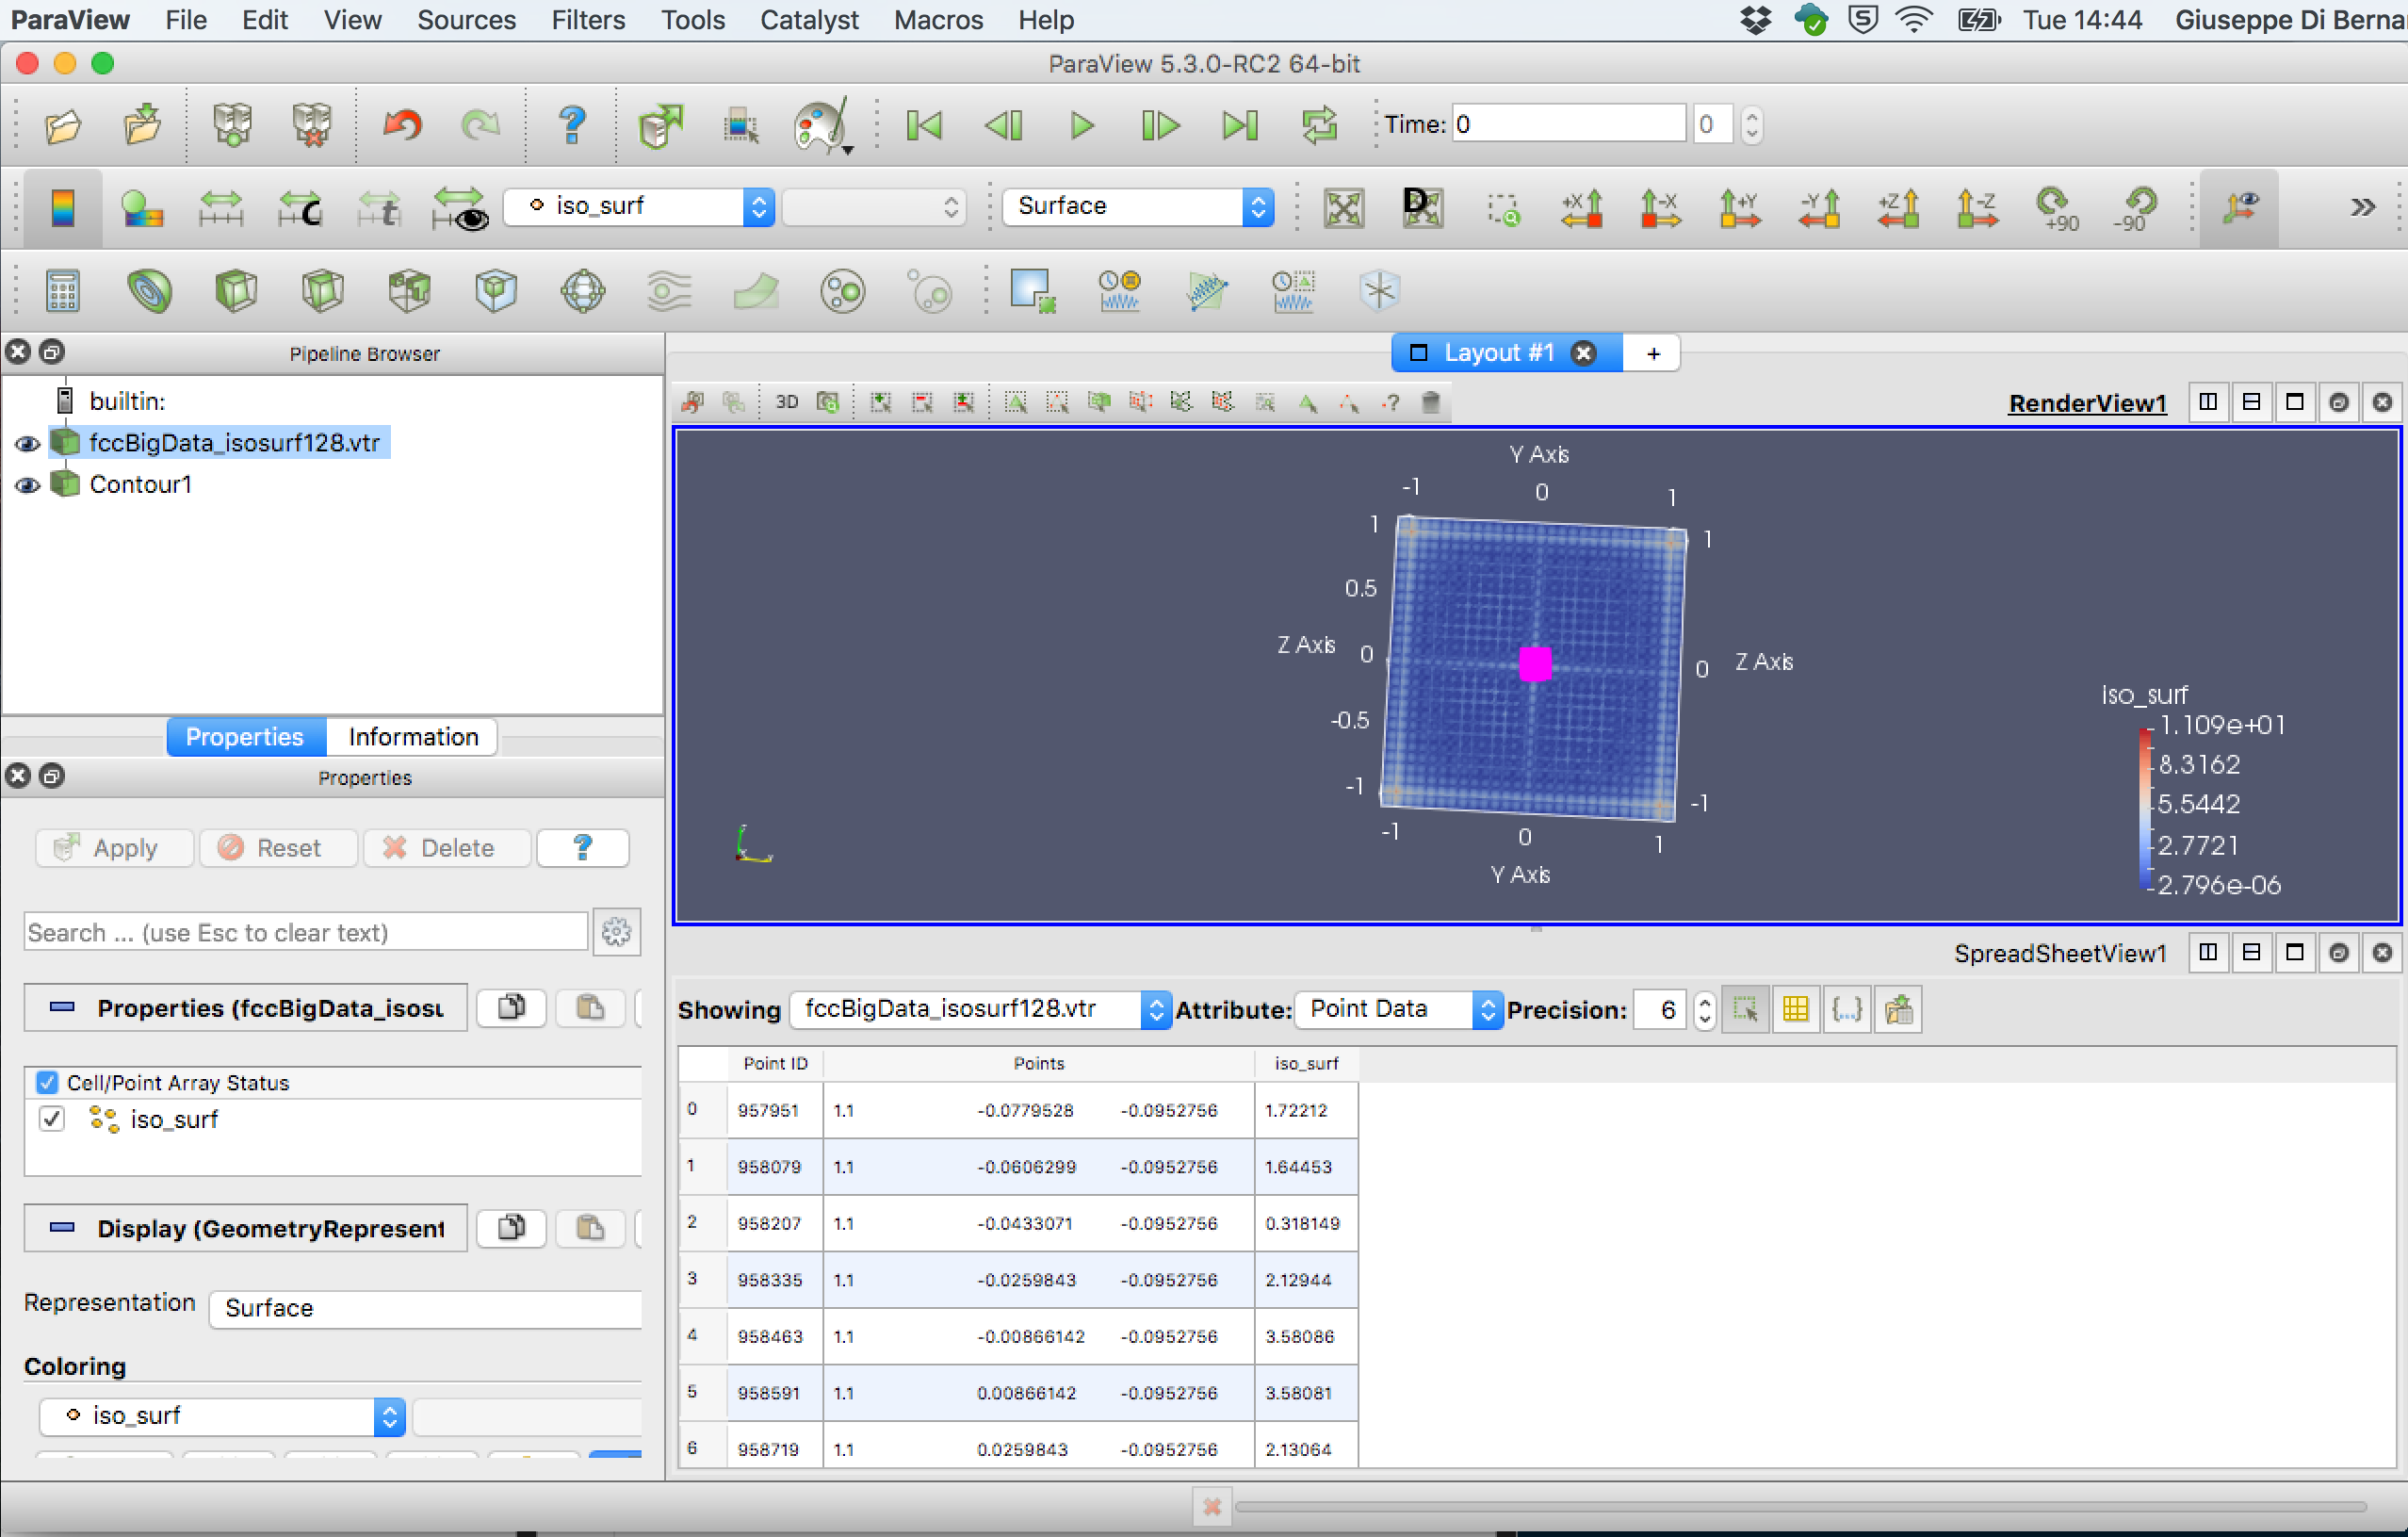
\includegraphics[width=.9\textwidth]{pics/visual_query}
% \frametitle{Theorem}
% \begin{theorem}[Mass--energy equivalence]
% $E = mc^2$
% \end{theorem}
\end{frame}

%------------------------------------------------

\begin{frame}
\frametitle{Hands-On: extract the tuple of radius and angles}
% \tdplotsetmaincoords{70}{110}
% \begin{tikzpicture}[tdplot_main_coords]
% \draw[thick,->] (0,0,0) -- (3,0,0) node[anchor=north east]{$x$};
% \draw[thick,->] (0,0,0) -- (0,3,0) node[anchor=north west]{$y$};
% \draw[thick,->] (0,0,0) -- (0,0,3) node[anchor=south]{$z$};
% \pgfmathsetmacro{\ax}{1}
% \pgfmathsetmacro{\ay}{1}
% \pgfmathsetmacro{\az}{1}
% \draw[->,red] (0,0,0) -- (\ax,\ay,\az);
% \draw[dashed,red] (0,0,0) -- (\ax,\ay,0) -- (\ax,\ay,\az);
% \tdplotgetpolarcoords{\ax}{\ay}{\az}
% \tdplotsetthetaplanecoords{\tdplotresphi}
% \tdplotdrawarc[tdplot_rotated_coords]{(0,0,0)}{1}{0}%
% {\tdplotrestheta}{anchor=west}{$\theta = \tdplotrestheta$}
% \end{tikzpicture}
\begin{columns}[c] 
 \column{.35\textwidth}
\tdplotsetmaincoords{60}{110}
%
\pgfmathsetmacro{\rvec}{.8}
\pgfmathsetmacro{\thetavec}{30}
\pgfmathsetmacro{\phivec}{60}
%
% \hspace*{1.05cm}
\begin{tikzpicture}[scale=4,tdplot_main_coords]
\coordinate (O) at (0,0,0);
\draw[thick,->] (0,0,0) -- (1,0,0) node[anchor=north east]{$x$};
\draw[thick,->] (0,0,0) -- (0,1,0) node[anchor=north west]{$y$};
24
\draw[thick,->] (0,0,0) -- (0,0,1) node[anchor=south]{$z$};
\tdplotsetcoord{P}{\rvec}{\thetavec}{\phivec}
\draw[-stealth,color=red] (O) -- (P);
\draw[dashed, color=red] (O) -- (Pxy);
\draw[dashed, color=red] (P) -- (Pxy);
\tdplotdrawarc{(O)}{0.2}{0}{\phivec}{anchor=north}{$\phi$}
\tdplotsetthetaplanecoords{\phivec}
\tdplotdrawarc[tdplot_rotated_coords]{(0,0,0)}{0.5}{0}%
{\thetavec}{anchor=south west}{$\theta$}
\draw[dashed,tdplot_rotated_coords] (\rvec,0,0) arc (0:90:\rvec);
\draw[dashed] (\rvec,0,0) arc (0:90:\rvec);
\tdplotsetrotatedcoords{\phivec}{\thetavec}{0}
\tdplotsetrotatedcoordsorigin{(P)}
% \draw[thick,tdplot_rotated_coords,->] (0,0,0)
% -- (.5,0,0) node[anchor=north west]{$x’$};
% \draw[thick,tdplot_rotated_coords,->] (0,0,0)
% -- (0,.5,0) node[anchor=west]{$y’$};
% \draw[thick,tdplot_rotated_coords,->] (0,0,0)
% -- (0,0,.5) node[anchor=south]{$z’$};
% \draw[-stealth,color=blue,tdplot_rotated_coords] (0,0,0) -- (.2,.2,.2);
% \draw[dashed,color=blue,tdplot_rotated_coords] (0,0,0) -- (.2,.2,0);
% \draw[dashed,color=blue,tdplot_rotated_coords] (.2,.2,0) -- (.2,.2,.2);
% \tdplotdrawarc[tdplot_rotated_coords,color=blue]{(0,0,0)}{0.2}{0}%
% {45}{anchor=north west,color=black}{$\phi’$}
% \tdplotsetrotatedthetaplanecoords{45}
% \tdplotdrawarc[tdplot_rotated_coords,color=blue]{(0,0,0)}{0.2}{0}%
% {55}{anchor=south west,color=black}{$\theta’$}
\end{tikzpicture}
\column{.65\textwidth}
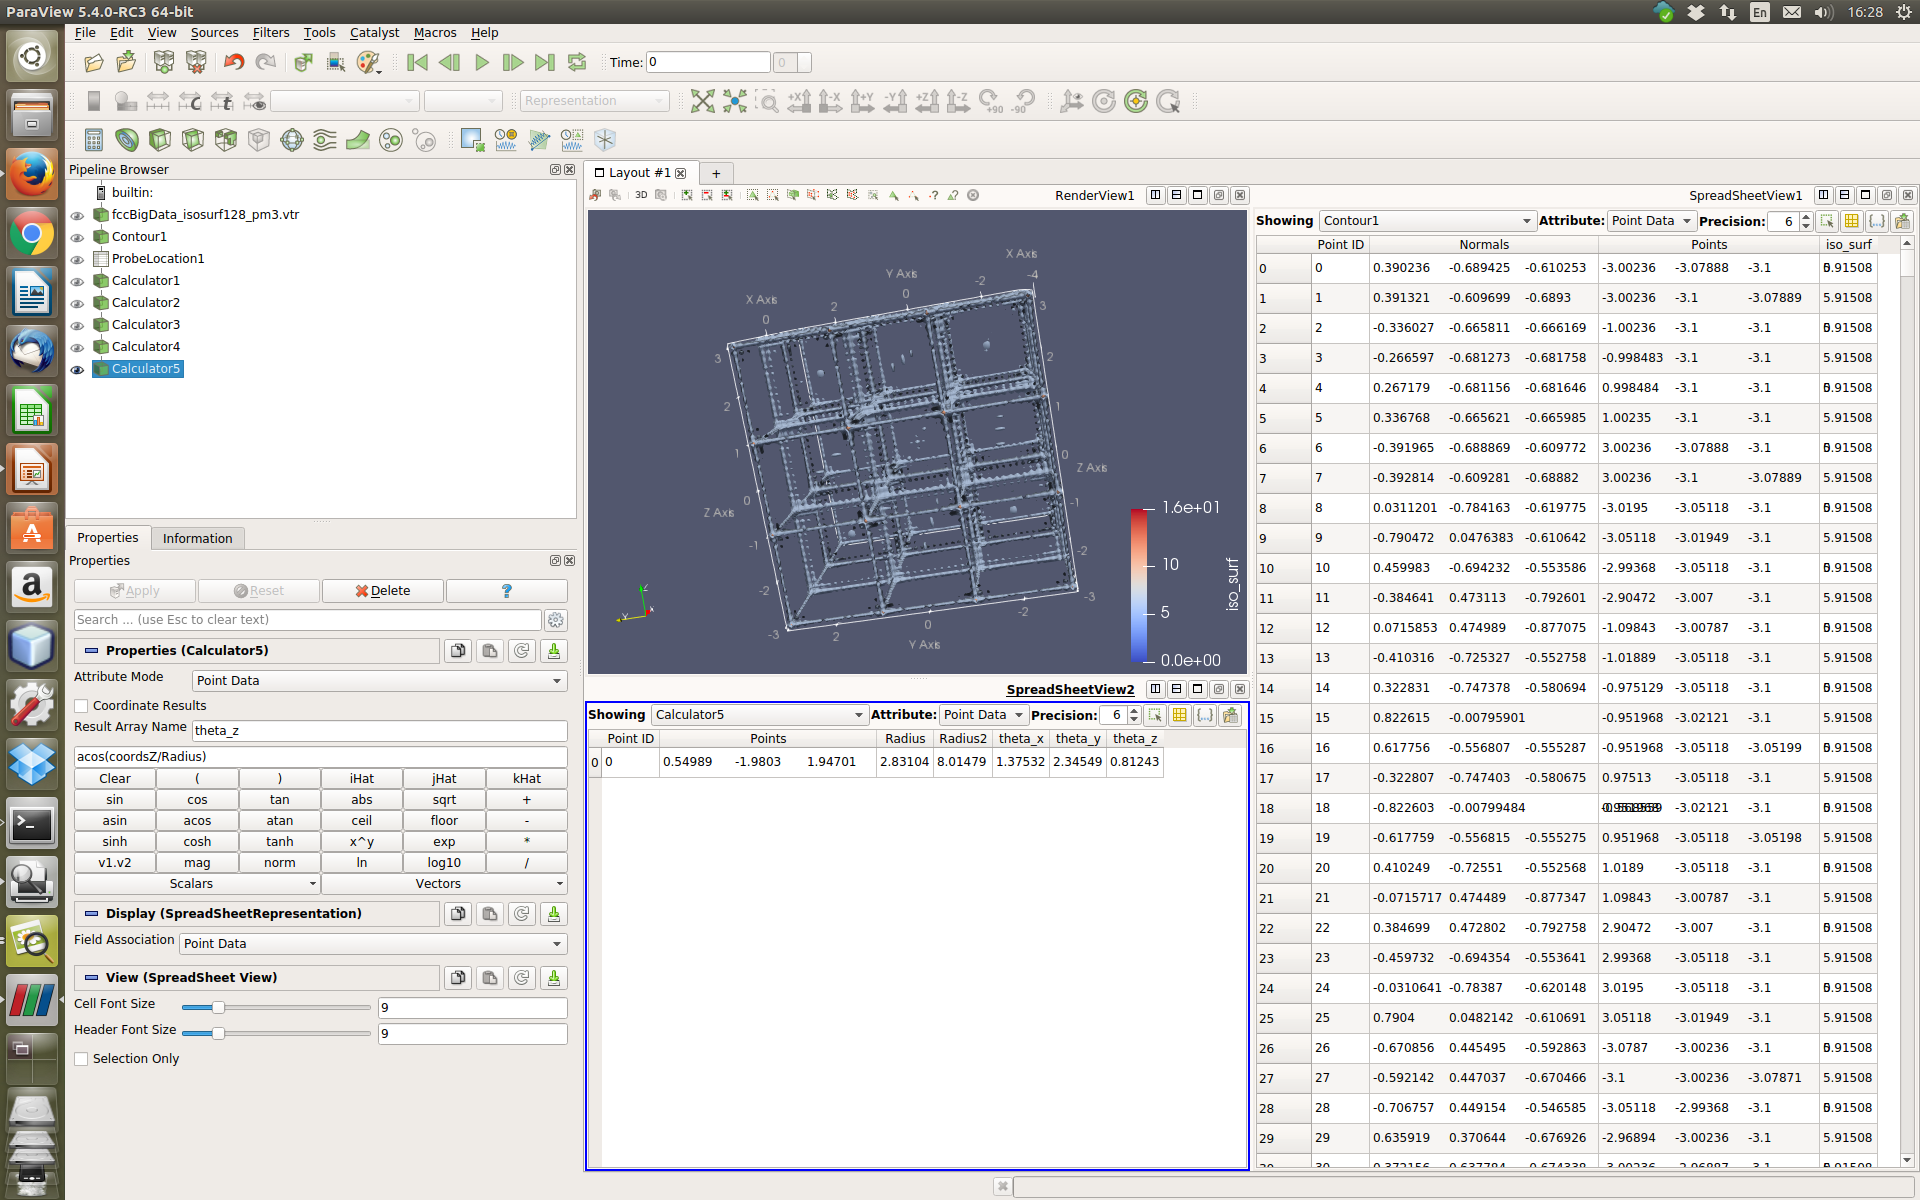
\includegraphics[width=1.2\textwidth]{pics/angles_tuple}
\vspace*{2.cm}
\hspace*{13cm}
\end{columns}

\end{frame}

% \begin{frame}
% \frametitle{Table}
% \begin{table}
% \begin{tabular}{l l l}
% \toprule
% \textbf{Treatments} & \textbf{Response 1} & \textbf{Response 2}\\
% \midrule
% Treatment 1 & 0.0003262 & 0.562 \\
% Treatment 2 & 0.0015681 & 0.910 \\
% Treatment 3 & 0.0009271 & 0.296 \\
% \bottomrule
% \end{tabular}
% \caption{Table caption}
% \end{table}
% \end{frame}

% %------------------------------------------------

% \begin{frame}
% \frametitle{Theorem}
% \begin{theorem}[Mass--energy equivalence]
% $E = mc^2$
% \end{theorem}
% \end{frame}

% %------------------------------------------------

% \begin{frame}[fragile] % Need to use the fragile option when verbatim is used in the slide
% \frametitle{Verbatim}
% \begin{example}[Theorem Slide Code]
% \begin{verbatim}
% \begin{frame}
% \frametitle{Theorem}
% \begin{theorem}[Mass--energy equivalence]
% $E = mc^2$
% \end{theorem}
% \end{frame}\end{verbatim}
% \end{example}
% \end{frame}

% %------------------------------------------------

% \begin{frame}
% \frametitle{Figure}
% Uncomment the code on this slide to include your own image from the same directory as the template .TeX file.
% %\begin{figure}
% %\includegraphics[width=0.8\linewidth]{test}
% %\end{figure}
% \end{frame}

% %------------------------------------------------

% \begin{frame}[fragile] % Need to use the fragile option when verbatim is used in the slide
% \frametitle{Citation}
% An example of the \verb|\cite| command to cite within the presentation:\\~

% This statement requires citation \cite{p1}.
% \end{frame}

% %------------------------------------------------

% \begin{frame}
% \frametitle{References}
% \footnotesize{
% \begin{thebibliography}{99} % Beamer does not support BibTeX so references must be inserted manually as below
% \bibitem[Smith, 2012]{p1} John Smith (2012)
% \newblock Title of the publication
% \newblock \emph{Journal Name} 12(3), 45 -- 678.
% \end{thebibliography}
% }
% \end{frame}

%------------------------------------------------

\begin{frame}
\Huge{\centerline{The End}}
\end{frame}

%----------------------------------------------------------------------------------------

\end{document}